\documentclass[a4paper]{ctexart}
\usepackage{xeCJK}
\usepackage{setspace}
\usepackage{graphicx,wrapfig}
\usepackage{fontspec,xunicode,xltxtra}
\usepackage{fancyhdr,titlesec,titletoc}
\usepackage[titletoc]{appendix}
\usepackage[top=29mm,bottom=29mm,left=31.8mm,right=31.8mm]{geometry}
\usepackage{enumerate,enumitem}
\usepackage{caption}
\usepackage{amsmath,amssymb,bm,array}
\usepackage{cite}
\usepackage{diagbox}
\usepackage{algorithm,algorithmicx,algpseudocode}
\usepackage{multirow}
\usepackage{listings}
\usepackage{color}
\setmainfont{Times New Roman}
\setCJKmainfont[BoldFont={Songti SC Bold}]{SimSun}
\setCJKfamilyfont{heiti}{SimHei}
\renewcommand{\heiti}{\CJKfamily{heiti}\fontspec{Times New Roman}}

\newcommand{\mycaptionfont}{\heiti\zihao{5}}
\captionsetup[figure]{name={\mycaptionfont 图},labelsep=period}
\captionsetup[table]{name={\mycaptionfont 表},labelsep=period}
\floatname{algorithm}{\mycaptionfont 算法}
\captionsetup[algorithm]{labelsep=period}
\renewcommand{\captionfont}{\mycaptionfont}
\renewcommand{\captionlabelfont}{\mycaptionfont}

\ctexset {
	section = {
		number = \arabic{section},
		format = \zihao{4}\bfseries,
	},
	subsection = {
		number = \arabic{section}.\arabic{subsection},
		format = \zihao{-4}\bfseries,
	},
	subsubsection = {
		number = \arabic{section}.\arabic{subsection}.\arabic{subsubsection},
		format = \zihao{-4}\bfseries,
	}
}
\setlist[enumerate]{itemindent=2em,listparindent=2em,leftmargin=1em,label=\arabic*、}

\setlength\parskip{.5\baselineskip}
\fancypagestyle{plain}{\pagestyle{fancy}}%改变章节首页页眉
\pagestyle{fancy}
\lhead{\kaishu~物联网综合课程设计~}
\rhead{\kaishu~尹达恒~伍华杰~纪港~孙硕}
\cfoot{\thepage}

\definecolor{codegreen}{rgb}{0,0.6,0}
\definecolor{codegray}{rgb}{0.5,0.5,0.5}
\definecolor{codepurple}{rgb}{0.58,0,0.82}
\definecolor{backcolour}{rgb}{0.95,0.95,0.92}

\titlecontents{section}[0em]{\vspace{0.01\baselineskip}\songti\zihao{-4}}{\thecontentslabel\ }{}
{\hspace{.5em}\titlerule*[4pt]{$\cdot$}\contentspage}
\titlecontents{subsection}[2em]{\vspace{0.01\baselineskip}\songti\zihao{-4}}{\thecontentslabel\ }{}
{\hspace{.5em}\titlerule*[4pt]{$\cdot$}\contentspage}
\setcounter{tocdepth}{2}

\begin{document}

\lstset{
	language={C},
	numbers=left,numberstyle=\tiny,
	basicstyle=\small\ttfamily,
	stringstyle=\color{codepurple},
	keywordstyle=\color{blue}\bfseries,
	commentstyle=\color{codegreen},
	rulesepcolor=\color{codegray},
	tabsize=2
}

\begin{spacing}{1}
	\tableofcontents
\end{spacing}
\newpage
\setcounter{page}{1}
\begin{center}
	{\zihao{-3}\textbf{基于树莓派和云服务的停车场道闸控制系统设计}}

	{\zihao{-4}尹达恒\quad 伍华杰\quad 纪港\quad 孙硕}\\[-1mm]

	{\zihao{5}(江南大学物联网工程学院,江苏\quad 无锡)}
\end{center}
\renewcommand{\baselinestretch}{1.3}
\songti\zihao{-4}
\section{设计要求}
\begin{itemize}
	\item 使用树莓派和传感器实现对车辆的感知、识别、信息上传和对闸杆的控制;
	\item 部署云服务系统实现车牌识别和车辆出入情况记录,并在网页上进行显示;
	\item 对树莓派和云服务系统进行整合,使之成为一个能协调工作的完整物联网系统。
\end{itemize}

\section{设计原理}
\subsection{红外传感器工作原理}
红外传感器是能将红外辐射能转换为电能的光敏器件。

红外线是太阳光线中众多不可见光线中的一种,与所有电磁波一样,具有反射、折射、散射、干涉、吸收等性质。利用红外线可以被物体反射这一性质,在一定范围内,反射管发射出一定频率的红外线,如果检测方向上没有障碍物,发射出去的红外线,因为传播的距离越来越远而逐渐减弱,最后消失;当检测方向存在障碍物时,发射出去的红外线反射回来被接收管接收,进而改变红外传感器输出电平,由此判断检测方向上是否存在障碍物。

\subsection{步进电机工作原理}
在额定负载一定时,步进电机停止的位置取决于输入脉冲信号的数量,而步进电机运行的速度取决于脉冲信号的频率。在实际使用中,负载的变化不会对两项参数造成很大影响。在输入端给与适当的脉冲信号时,转子会以一定的方式旋转;输入端无脉冲信号时,转子会保持当前的位置不动。步进电机工作的基本原理如下:
\begin{enumerate}
	\item 换相顺序的控制

		  步进电机上电后,工作相序的控制取决于脉冲信号的分配。以最基本的四相八拍为例,要求的工作顺序为A-AB-B-BC-C-CD-D-DA,输入端的脉冲就会以A、B、C、D这种顺序进行相序的通断设置。还有四相四拍运行方式,即AB-BC-CD-DA-AB;
		  
	\item 步进电机转向的改变

	      如果要求电机正向转动,输入端就要按照正向的顺序为电机通电;同理如果要求电机反向转动,输入端就要按照相反的顺序来为电机通电;

	\item 步进电机转动速度的改变

	      每当输入端接收到一个脉冲信号,步进电机的转子就会转动一次,产生一定的转动角度。所以输入端两次脉冲的时间间隔决定步进电机的转动速度,两次脉冲发送间隔越长,对应的步进电机转动速度就越慢。如果需要对步进电机转动速度加以控制,就要对主控模块在单位时间内发出的脉冲个数进行控制。
	      本系统采用28BYJ-48四相五线式步进电机。电机公共端连接电源正极,电机剩余的四根控制线顺次与电源的接地端(此处可理解为负极)连接。接线时可以看到,每当电机控制线与电源地线接触一次,步进电机就会旋转一定角度。
\end{enumerate}

\subsection{中文车牌识别原理}
中文车牌识别,经过近二十年的发展,在特定场景下,已经具备了相对成熟的解决方案。如停车场卡口,小区入口等。车牌识别技术是现代智能交通系统重要组成部分,其应用十分广泛。它以计算机视觉处理、数字图像处理、模式识别等技术为基础,对摄像机所拍摄的车辆图像或者视频图像进行处理分析,得到每辆车的车牌号码,从而完成识别过程。车牌识别在高速公路车辆管理中得到广泛应用,如高速收费,交通违章检测等。在停车场管理中,车牌识别技术也是识别车辆身份的主要手段。

本项目中我们借鉴学习并改进使用了Github上一个比较优秀的开源方案HyperLPR。HyperLPR是一个使用深度学习针对对中文车牌识别的实现,与较为流行的开源的EasyPR相比,它的检测速度和鲁棒性和多场景的适应性更好,且可以识别多种中文车牌,包括白牌,新能源车牌,使馆车牌,教练车牌,武警车牌等。HyperLPR的优点主要有以下几条:
\begin{itemize}
	\item 速度快:720p,单核 Intel 2.2G CPU 平均识别时间低于100ms;
	\item 基于端到端的车牌识别无需进行字符分割;
	\item 识别率高:仅仅针对车牌ROI在EasyPR数据集上,0-error达到95.2\%,1-error识别率达到 97.4\% (指在定位成功后的车牌识别率);
	\item 轻量:总代码量不超1000行。
\end{itemize}

\subsection{长轮询通信原理}
长轮询(Long Polling)是一种HTTP实现的“服务器推”的技术,它弥补了HTTP简单的请求应答模式无法保证数据即时交互的不足,极大地增强了程序的实时性和交互性。长轮询一般应用与WebIM、ChatRoom和一些需要及时交互的网站应用中。其真实案例有:WebQQ、Hi网页版、Facebook IM等。

在长轮询中,客户端向服务器发送轮询请求,服务器接到请求后保持连接,直到有新消息才返回响应信息并关闭连接,客户端处理完响应信息后再向服务器发送新的轮询请求。与传统的HTTP请求应答模式不同,长轮询方式在无消息的情况下不会频繁的请求,且在服务器端有新消息回应时能立即接收,在降低了网页即时通信带宽消耗的同时极大地提升了消息传输的性能。

\subsection{微服务架构原理}
微服务架构(Microservice Architecture)是一种架构概念,旨在通过将功能分解到各个离散的服务中以实现对解决方案的解耦。微服务架构把一个大型的单个应用程序和服务拆分为数个甚至数十个支持微服务,它可扩展单个组件而不是整个的应用程序堆栈,从而满足服务等级协议。这些支持微服务可独立地进行开发、管理和迭代。在分散的组件中使用云架构和平台式部署、管理和服务功能,使产品交付变得更加简单。

Docker是针对微服务架构开发最具代表性的应用之一。它是一个基于PaaS (Platform as a Service:平台即服务)思想的开源应用容器引擎,让开发者可以打包他们的微服务应用以及相关的依赖包到一个可移植的容器中,然后使用虚拟化方法部署到任何安装了Docker的物理服务器上,容器是完全使用沙箱机制,相互之间不会有任何依赖接口。

基于Docker的软件交付运行环境如同海运,其中虚拟化的操作系统镜像(image)如同一个货轮,在其中运行的微服务如同一个个集装箱,用户可以通过标准化手段自由组装运行环境,集装箱的内容可以由用户自定义,也可以由专业人员制造。这样,交付软件就被分解为交付一系列标准化微服务集合,从而更有效地实现微服务架构开发。


\section{设计方案}
\subsection{道闸硬件设计}
根据设计要求,本系统选用了目前最新的树莓派3B+作为主控模块,配合红外传感器、摄像头、步进电机及对应驱动芯片完成系统设计与开发。

\subsubsection{主控模块}
主控模块是系统的控制机构和通信机构,主要负责控制子模块的运行,处理信息及发送指令;与云服务系统进行通信,上传待识别车牌图像等原始信息,并接受云端指令。

本次停车场道闸控制系统选择了基于ARM嵌入式平台、树莓派系列中最新一代的树莓派3B+作为主控模块。树莓派3B+开发板拥有良好的标准模块扩展性,具备多种规格的外接设备口,主板上预留的接口可与树莓派500万像素专用摄像头完美对接,同时兼容红外传感器、步进电机等其他硬件开发模块。树莓派3B+实物如图\ref{fig:树莓派3B+实物图}所示。

\begin{figure}[htbp]
	\centering
	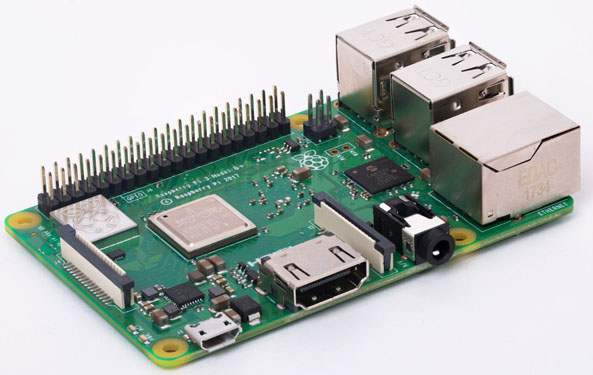
\includegraphics[width=\textwidth]{figure/hardware-RPI3B.jpg}
	\caption{树莓派3B+实物图}\label{fig:树莓派3B+实物图}
\end{figure}

树莓派3B+开发板是一款基于Broadcom BCM2837B0四核A53 CPU的多功能硬件开发平台,拥有1GB LPDDR2内存,采用Micro-SD作为外部存储,支持千兆以太网、2.4GHz和5GHz 双频Wi-Fi、蓝牙4.2,该开发板具有4个USB接口、一个以太网接口、HDMI高清视频输出接口、3.5mm模拟音频视频插孔、摄像机串行接口(CSI)、显示器串行接口(DSI)、40引脚GPIO双排插针,拥有强大的外接扩展能力和深度开发潜力。

树莓派将Python作为主要编程语言,支持java、BBC BASIC(通过RISCOS映像或者Linux的“Brandy Basic”克隆)、C和Perl等编程语言。本系统采用树莓派官方的最新Raspberry Pi系统(基于Linux32位操作系统开发而出),以Python作为编程语言完成系统开发。

\subsubsection{感应模块}
感应模块选用了红外传感器,其作用是检测车辆的到来,控制摄像头获取车牌图像,以及检测车辆是否通过道闸,道闸杆是否可以落下。红外传感器在待机状态时,持续输出为高电平;当红外传感器检测到物体时,会快速切换为工作模式,输出低电平;当物体被移开,红外传感器再次进入待机状态,输出高电平。红外传感器电路原理图如图\ref{fig:红外传感器原理图}所示。

\begin{figure}[htbp]
	\centering
	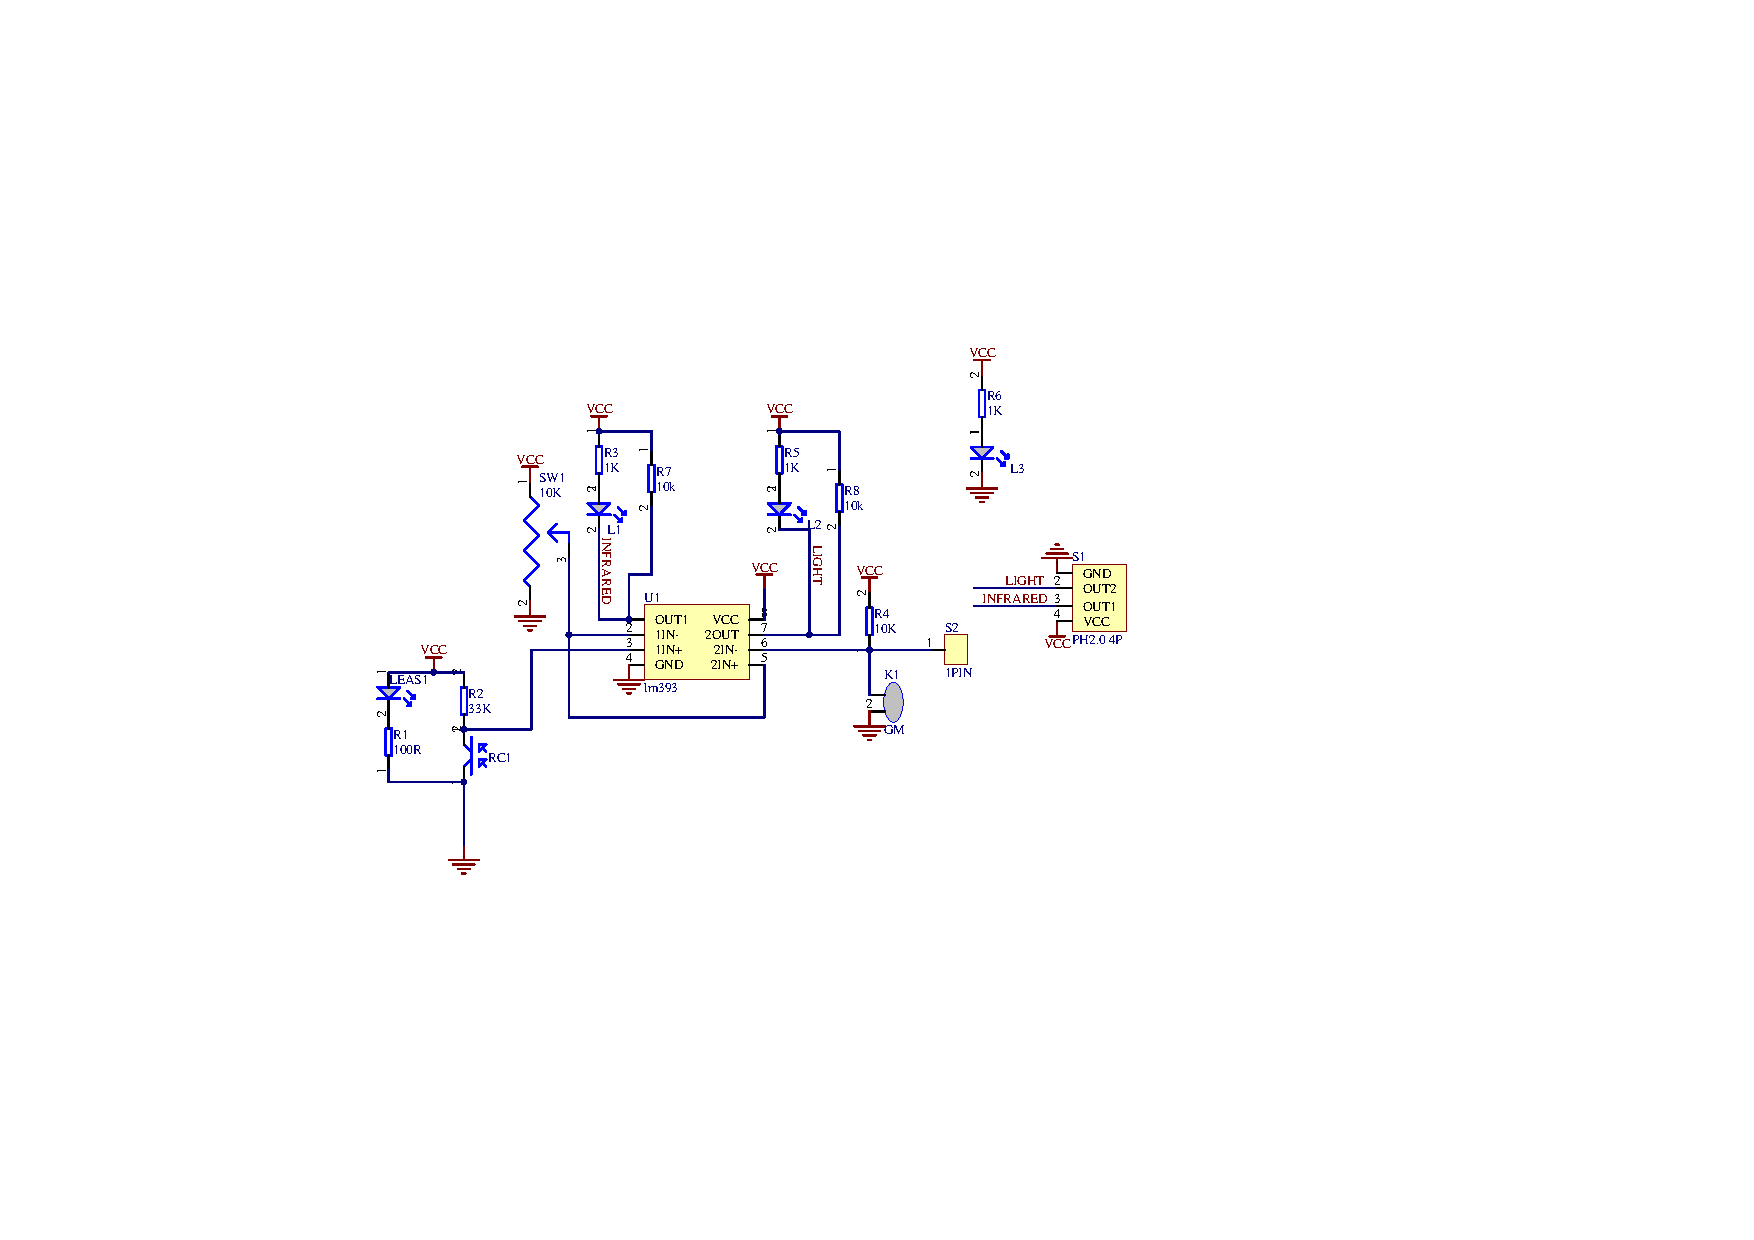
\includegraphics[width=\textwidth]{figure/hardware-red.pdf}
	\caption{红外传感器原理图}\label{fig:红外传感器原理图}
\end{figure}

\subsubsection{拍照模块}
拍照模块选用了树莓派专用500W像素摄像头(含CSI接口排线),该摄像头由OmniVision公司生产(基于OV5647图像处理传感模块),为树莓派专用拍照模块,兼容性更加优良。摄像头实物与参数如图\ref{fig:摄像头实物及参数图}所示。

\begin{figure}[htbp]
	\centering
	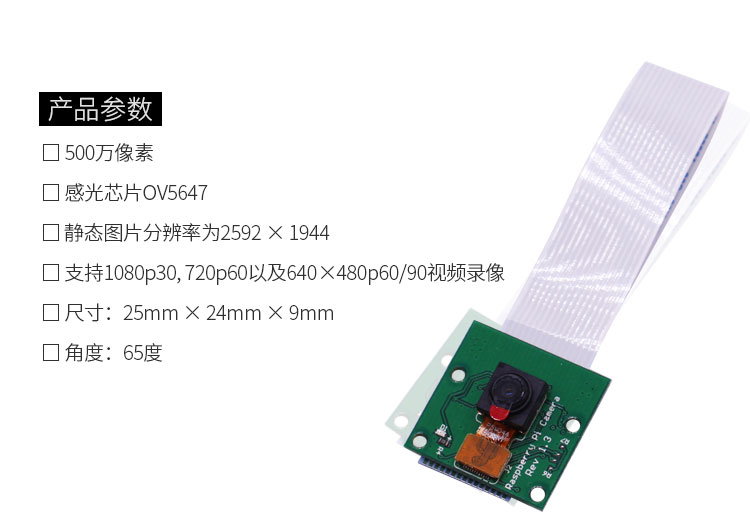
\includegraphics[width=\textwidth]{figure/hardware-camera.jpg}
	\caption{摄像头实物及参数图}\label{fig:摄像头实物及参数图}
\end{figure}

该拍照模块的核心元件是一个500W像素的CMOS传感器,支持最大分辨率为2592×1944的图片拍摄,同样支持每秒30帧的1080P视频拍摄(同时兼容每秒60帧的720P视频拍摄)。拍照模块与主控模块通过一条15芯的排线(CSI接口)进行连接。

\subsubsection{驱动模块}
由于树莓派的GPIO口驱动能力相对较弱,驱动电平仅为3.3V,所以高电平驱动比低电平驱动能力稍弱些。当主控模块直接将输入信号传递给步进电机时,步进电机无法正常工作,所以在本次设计中需要添加一个驱动模块。驱动模块具有放大功率的作用,可以满足在输入信号比较微弱、输出功率比较高的情况下工作。
考虑本系统实际,驱动模块主要需要满足以下要求:

\begin{itemize}
	\item 驱动电路提供的电流波形尽可能的接近矩形波,需要电流的快速上升及快速下降;
	\item 驱动电路输出的功率及运行的效率要求较高,使系统提高运行经济效率。
\end{itemize}

经过简单的比对,本系统设计拟采用ULN2003类的驱动IC(集成电路芯片),该芯片可为步进电机提供小于0.5A的电流。驱动芯片ULN2003内部结构如图\ref{fig:ULN2003内部控制单元原理图}所示。

\begin{figure}[htbp]
	\centering
	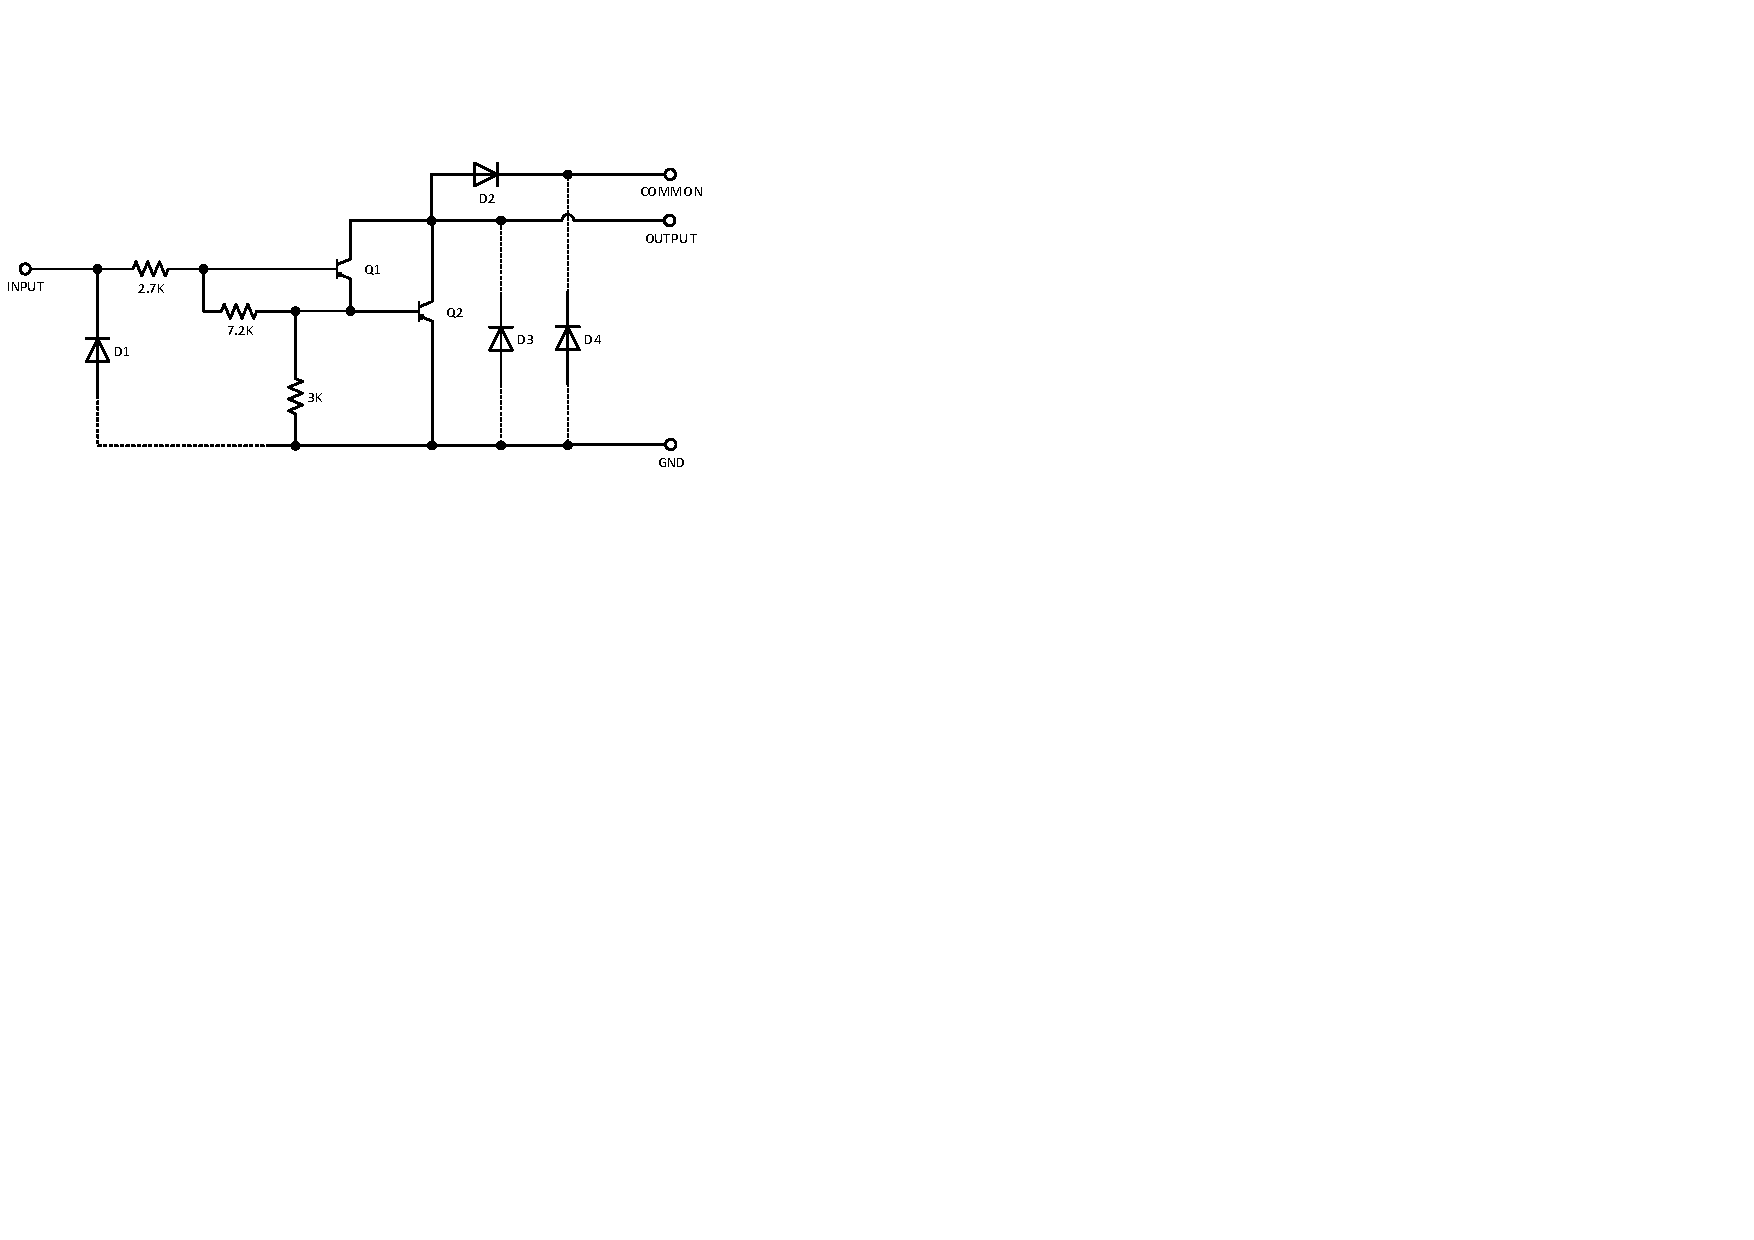
\includegraphics[width=\textwidth]{figure/hardware-cir.pdf}
	\caption{ULN2003内部控制单元原理图}\label{fig:ULN2003内部控制单元原理图}
\end{figure}

ULN2003芯片是由多个复合达林顿晶体管排列组成,这样的设计可以使耐受电压比较高,允许通过电流比较大。该芯片由7对NPN达林顿管组成,每个NPN达林顿管作为1个控制单元,其中7个控制单元包含功率驱动单元、保护单元等。ULN2003采用多种封装方式:如DIP-16或者SOP-16双列16脚塑料封装。驱动模块输出端可以与步进电动机直接连接,其内部数字逻辑电路为非门电路,采用取反的控制方式。

在满足以上要求的同时,系统还要稳定运行且性价比高,所以系统最终采用 ULN2003 作为电机驱动芯片。该芯片可以直接使用主控模块的GPIO口所提供的信号,硬件电路连接十分简单。该芯片采用树莓派作为控制核心,在进行程序相互调用时,操作起来也十分方便灵活。

ULN2003芯片的主要特点是:
\begin{itemize}
	\item ULN2003芯片驱动电流比较大,可以较好的用于单片机控制的电路。
	\item 为提高其抵抗干扰的能力,ULN2003可通过连接上拉电阻的方式,在驱动步进电机时抵御不必要的干扰。同时芯片内部每个控制单元都会串联高阻值的电阻,这样可以直接与TTL或承载电压为5V的CMOS装置连接。
	\item ULN2003输出端的电路集电极状态设置为开路状态,优点是电流的输出值比较大,峰值可以达到500mA,因此可以用来驱动步进电机。
\end{itemize}

ULN2003芯片引脚如图\ref{fig:ULN2003原理图}所示,输入部分为左侧1~7引脚,连接主控模块输出端(GPIO),由主控模块提供控制信号;引脚8直接接地;输出部分为右侧1~7引脚,与5V步进电机相连,必要时可以悬空而置,不做任何连接;引脚VCC接5V电源,该芯片可提供最高为0.5A的电流输出。

\begin{figure}[htbp]
	\centering
	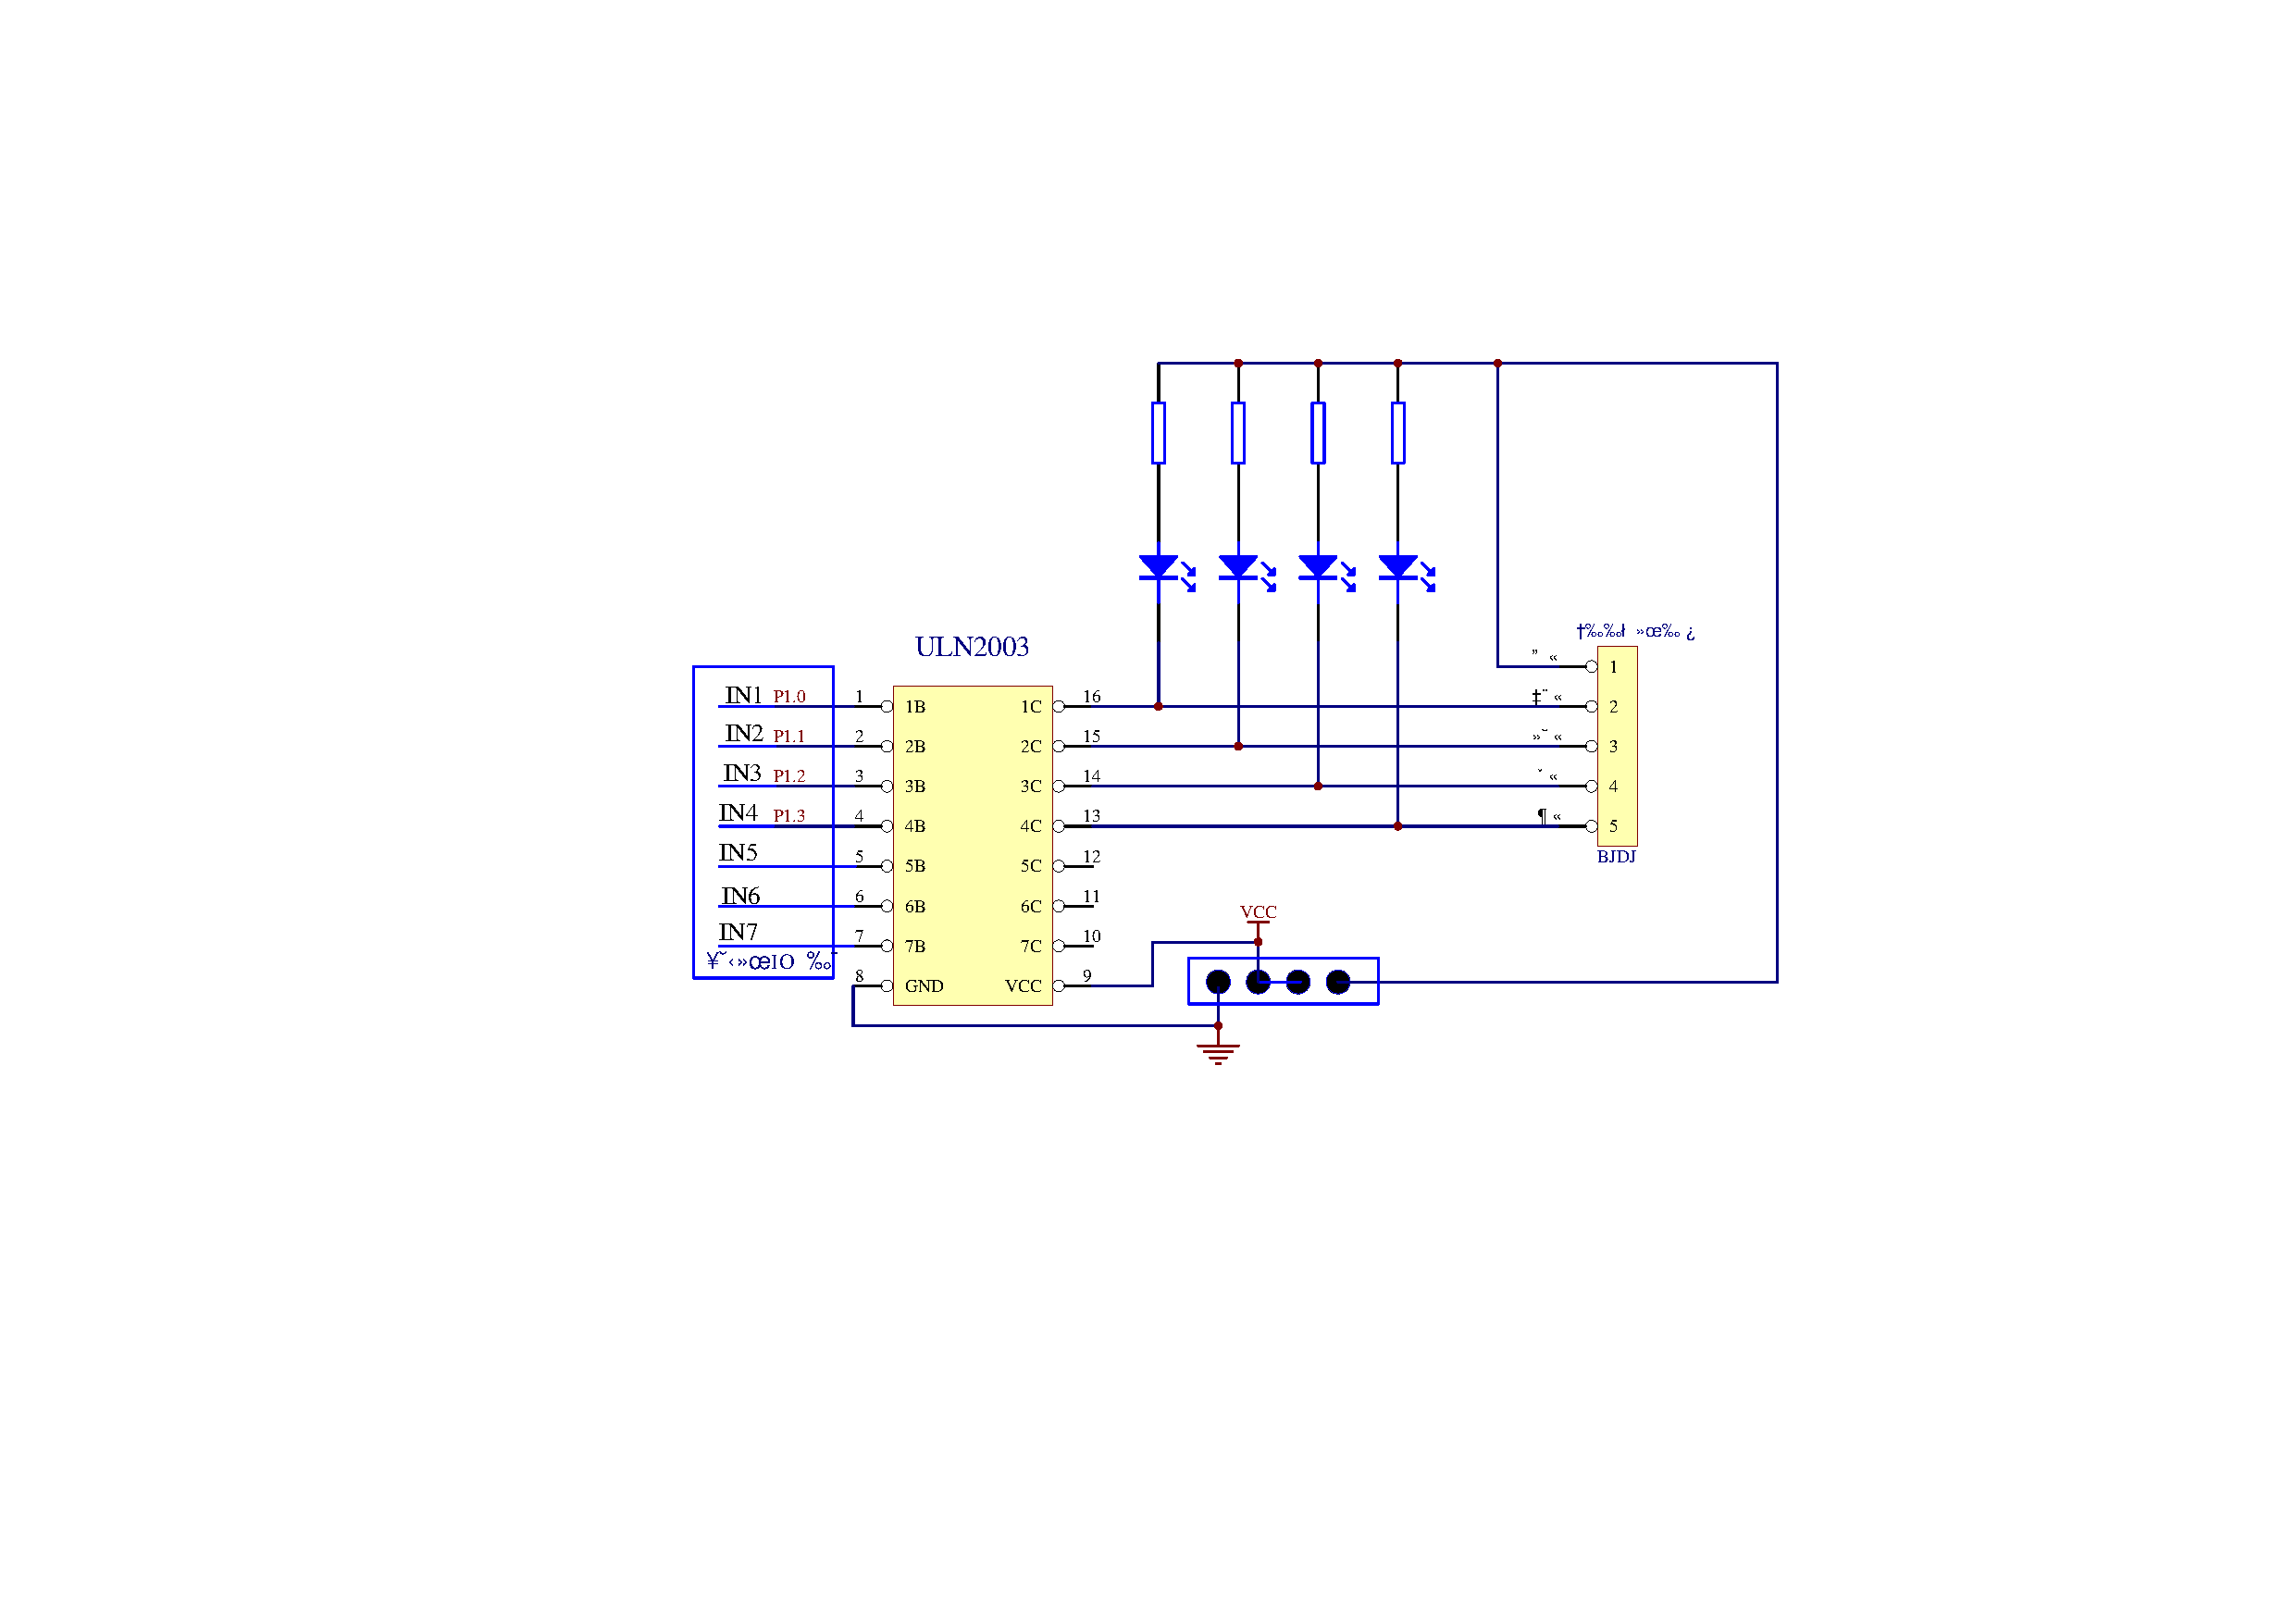
\includegraphics[width=\textwidth]{figure/hardware-pin.pdf}
	\caption{ULN2003原理图}\label{fig:ULN2003原理图}
\end{figure}

按照电路设计,步进电机输入端的红色线接VCC,其它线则用来连接驱动板。根据芯片资料,步进电机驱动芯片上有IN1~4四个接口,驱动方式为低电平供电,用杜邦线分别将 IN1,IN2,IN3,IN4 和GPIO 5(Pin 29),GPIO 6(Pin 31),GPIO 13(Pin 33),GPIO 19(Pin 35)进行连接。每次将四个GPIO端口按表2-3(步进电机驱动原理表)依次设置好电平后,可以通过设置sleep函数的时间来控制转速。

\subsubsection{电机模块}
步进电机属于电机中一个独特的类别,有别于常见的电机,该类别的电机具有精准控制的功能,可同时控制位置与速度两个矢量。与其他控制类电机不同的是,该种电机的控制方式采用开环控制(无反馈环节),可将输入端微弱且间断的触发脉冲信号转变成电机转动的线位移或者角位移。控制方式采用数字信号进行控制,短暂的脉冲信号就可对电机实现控制,随即转化为相应的角位移。由上得知,只要在步进电机输入端加以一个适当的脉冲信号,然后就会输出固定的角度,该种控制方式对开发者来说编程简单,操作可见性高。步进电机的相数取决于绕在定子的线圈数量,可分为两相、四相、五相等;步进电机的线式取决于电机的外部引线,分为三线式、五线式、六线式等。根据相数、线式、功能、用途的不同,步进电机分为多种类型,但是电机本身的控制方法均通过脉冲信号进行控制,没有很大的区分。

考虑到道闸系统的实际使用情况,运动过程中不需要加速、减速过程,同时对转速的要求也比较低,所以将步进电机设置为自启动运行方式。自启动运行方式是指通过控制脉冲速度,从而控制电机的启动和停止的运行方式,该种运行方式不会产生加速或者减速阶段。由于在道闸系统的开启、闭合时需要速度的突然变化,所以需要较大的转矩。同时在实际使用过程中电机有一定的负载,会产生较大的工作噪音,根据常见步进电机的工作特性,只有四相五线式步进电机的满足工作需求。另外考虑到静转矩、步距角、电流、安装难度等多种因素,本系统选取28BYJ-48四相五线式步进电机对道闸系统进行控制。

\subsection{道闸软件设计}
系统采用py语言编程,软件使用主控模块树莓派定制版本,将程序模块化,便于功能的进一步扩展,模块化还有利于错误的检查和后期的优化。完整的停车管理系统的道闸设计包含主程序的设计、拍照模块的程序设计、驱动模块的程序设计。

\subsubsection{主程序模块的设计}

主控模块通电后立即进入系统并且连接上WiFi无线网络,在搭建好运行环境以及经过代码调试之后,启动进车程序。在进车程序中,车缓缓停下准备入库。若此时第一个红外检测到车身经过,则摄像头开启抓捕拍照,而且仅仅拍一张照片,将其存放到树莓派本地。紧接着照片被送往云端识别,会立即返回车的车牌号码。可能会出现未识别的情况,只要车不退回,系统会一直拍照直至能够产生车牌号码,除非用户自己离开系统放弃拍照。若产生正确的照片会被发往停车管理系统云端,返回剩余车位不为0时则杆立即抬起,车开始开进车库,第二个红外模块检测到车身时直至检测不到杆落下。整个进库的流程图如图\ref{fig:车入库主程序流程图}所示。

\begin{figure}[htbp]
	\centering
	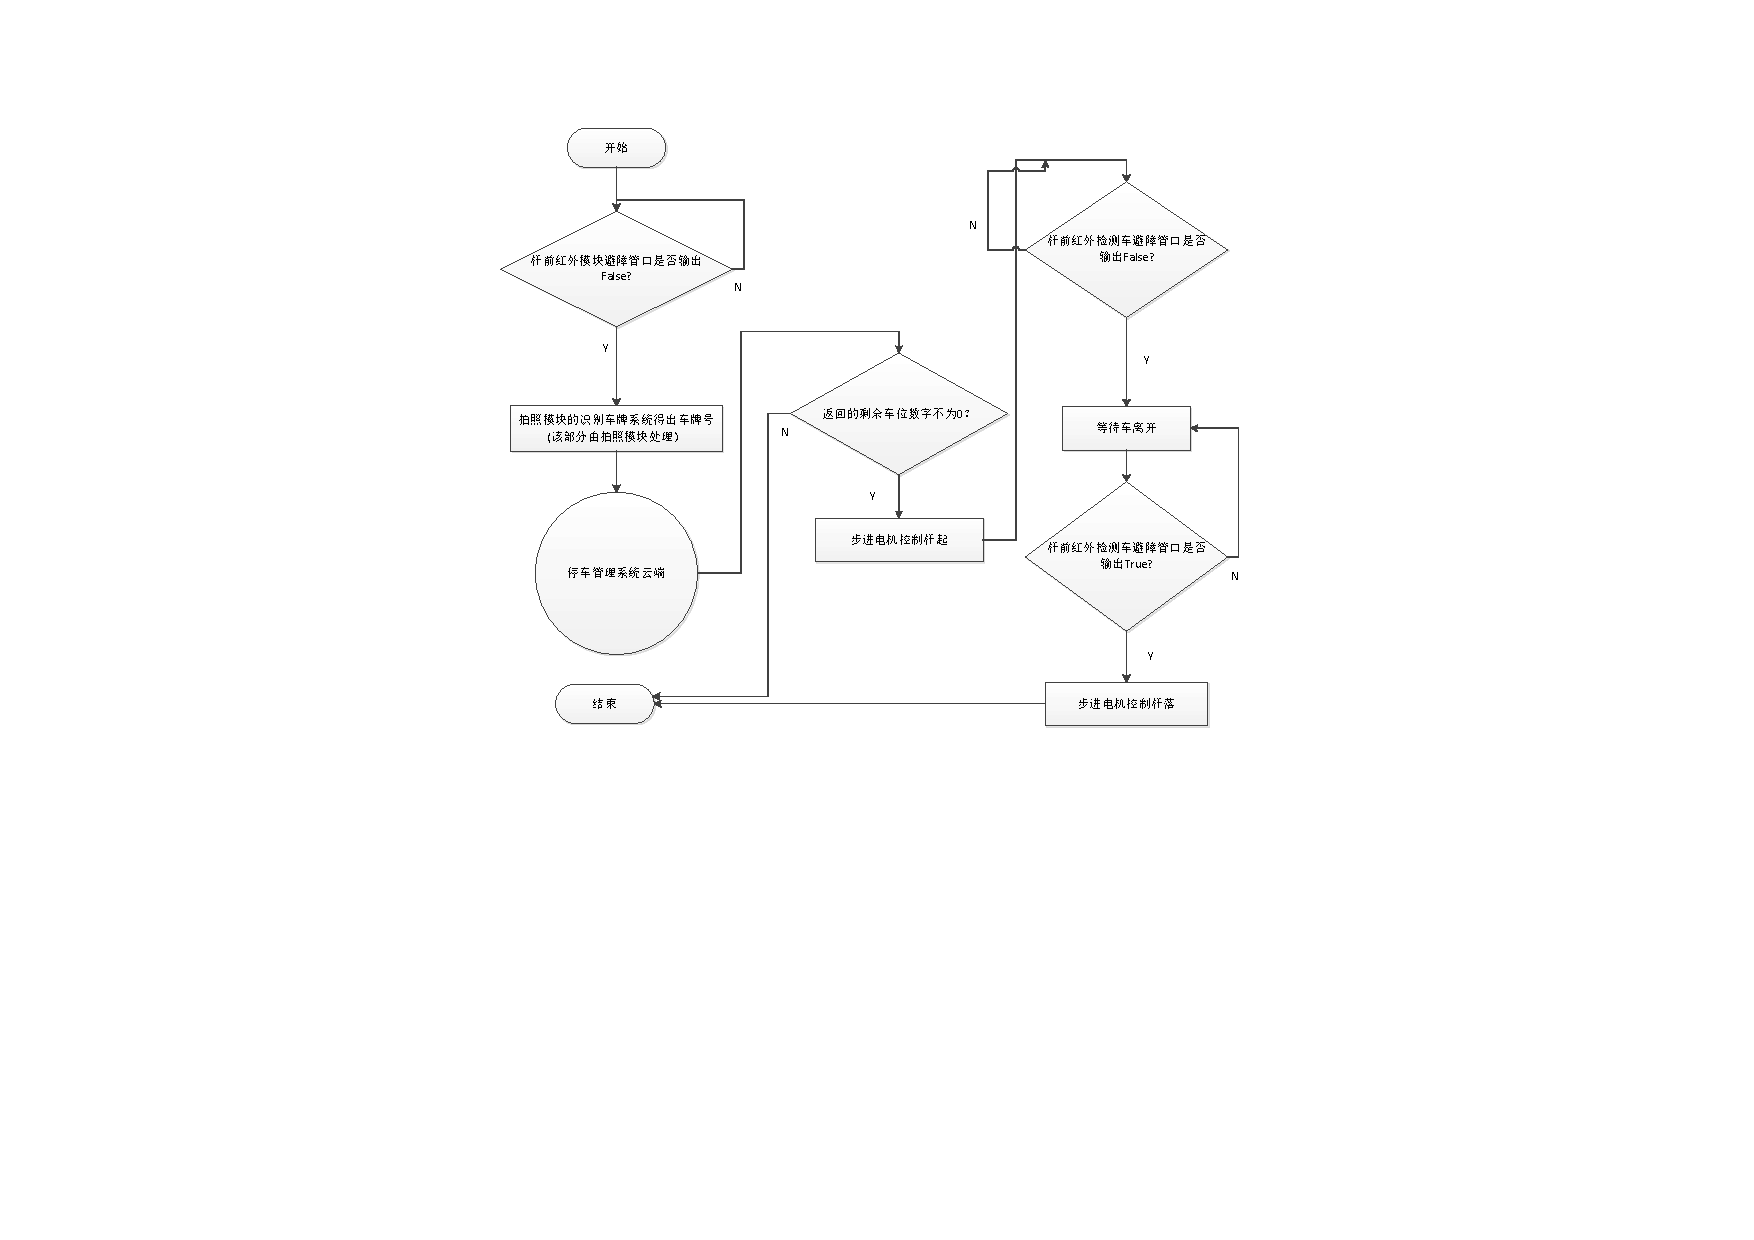
\includegraphics[width=\textwidth]{figure/software-1.pdf}
	\caption{车入库主程序流程图}\label{fig:车入库主程序流程图}
\end{figure}

出库程序运行时,当红外模块检测到车身时,则摄像头开启抓捕拍照。类似于车进库的操作,照片被送往云端识别,云端会返回车的号码。若是没有识别会会一直识别,若是长久不能识别,车主此时必须打电话给管理员。若是车牌识别成功,会立即发往停车管理系统云端,云端返回一个SVG字符串格式的二维码。
在本地将此格式转换为jpg图片格式即为付款二维码。车主需要付款扫二维码并付款成功后杆才可抬起,离开的时候第二个红外模块第一次检测到车身不落杆,直到避障管脚输入True时,杆才开始落下,此时车已经安全离开。车出库主程序流程图如图\ref{fig:车出库主程序流程图}所示。
 
\begin{figure}[htbp]
	\centering
	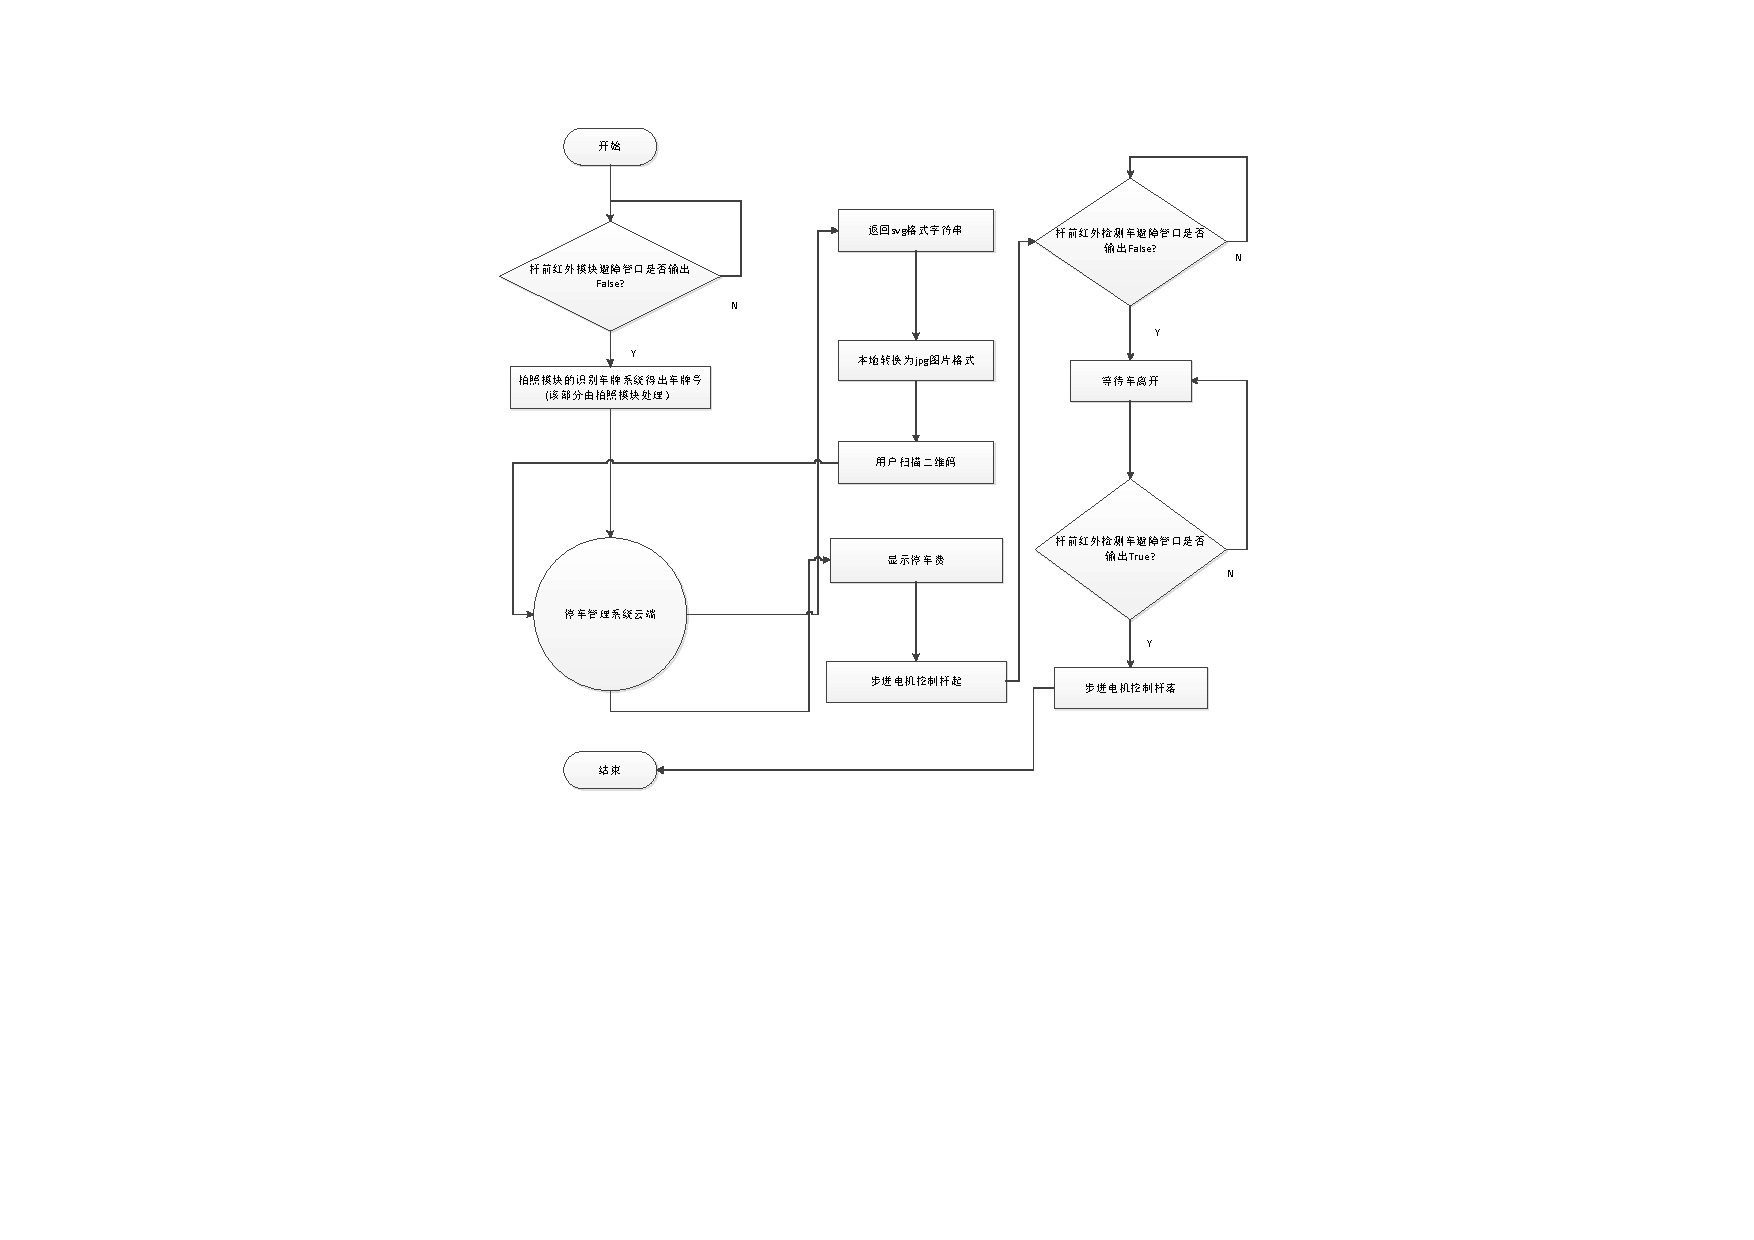
\includegraphics[width=\textwidth]{figure/software-2.pdf}
	\caption{车出库主程序流程图}\label{fig:车出库主程序流程图}
\end{figure}

\subsubsection{拍照模块的设计}
车进库初次进入系统将拍照模块功能设置为enabled,以便程序调用。在本次的设计中,程序本想利用OpenCV进行照片的处理,但因为网络的问题无法下载OpenCV程序包,故利用云端识别的方法从云端返回识别的图片。调用进行拍照处理。当拍照模块的拍照服务启动时,将采集的图片保存为jpg格式,然后等待下次调用拍照模块程序设计流程图如图\ref{fig:入库拍照模块程序设计流程图}所示。
 
\begin{figure}[htbp]
	\centering
	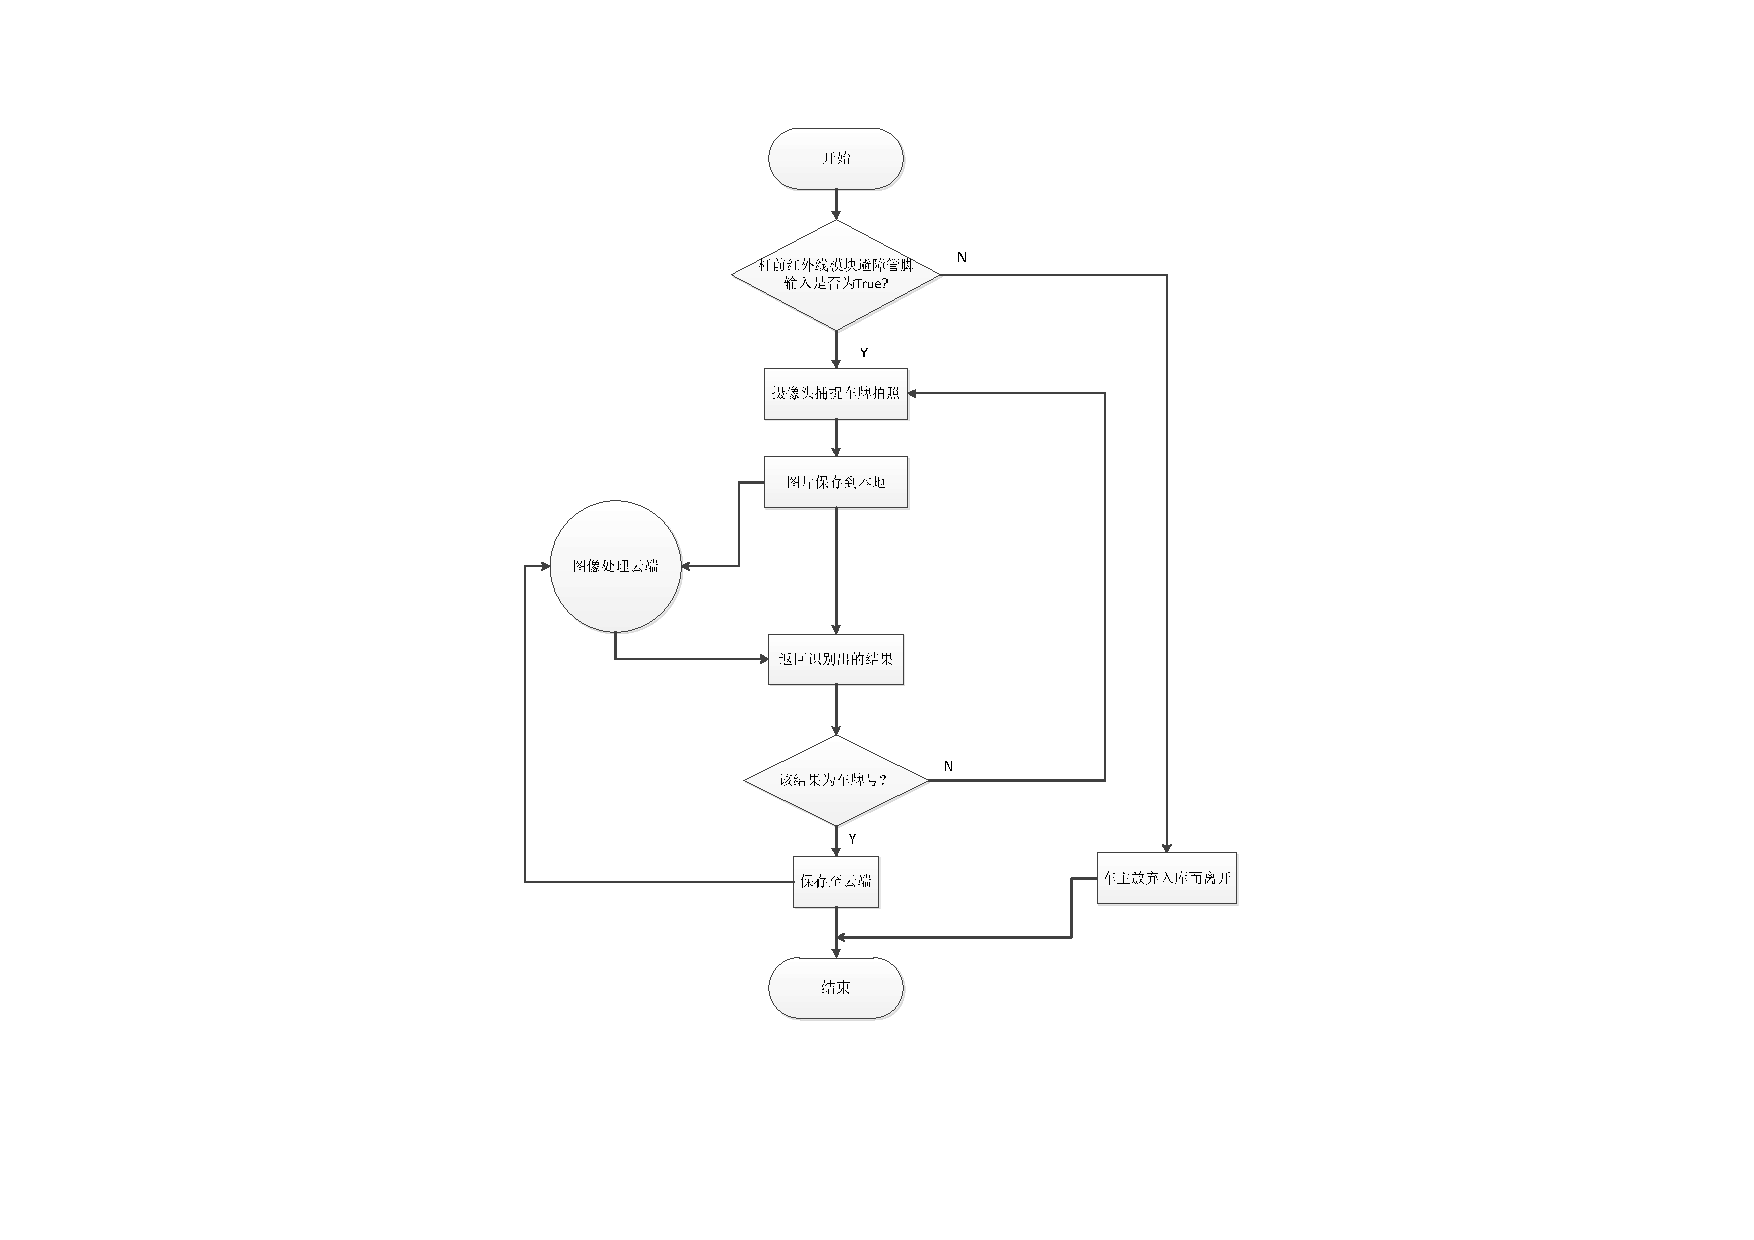
\includegraphics[width=\textwidth]{figure/software-3.pdf}
	\caption{入库拍照模块程序设计流程图}\label{fig:入库拍照模块程序设计流程图}
\end{figure}

车出库与进库拍照模块程序基本一致,有一点不一样,车入库时若是照片一直无法识别,车主可以选择离开,大不了换其他停车场。但是若是出库时照片识别不,车主只能打电话给管理员。出库拍照模块程序设计流程图如图\ref{fig:出库拍照模块程序设计流程图}所示。

\begin{figure}[htbp]
	\centering
	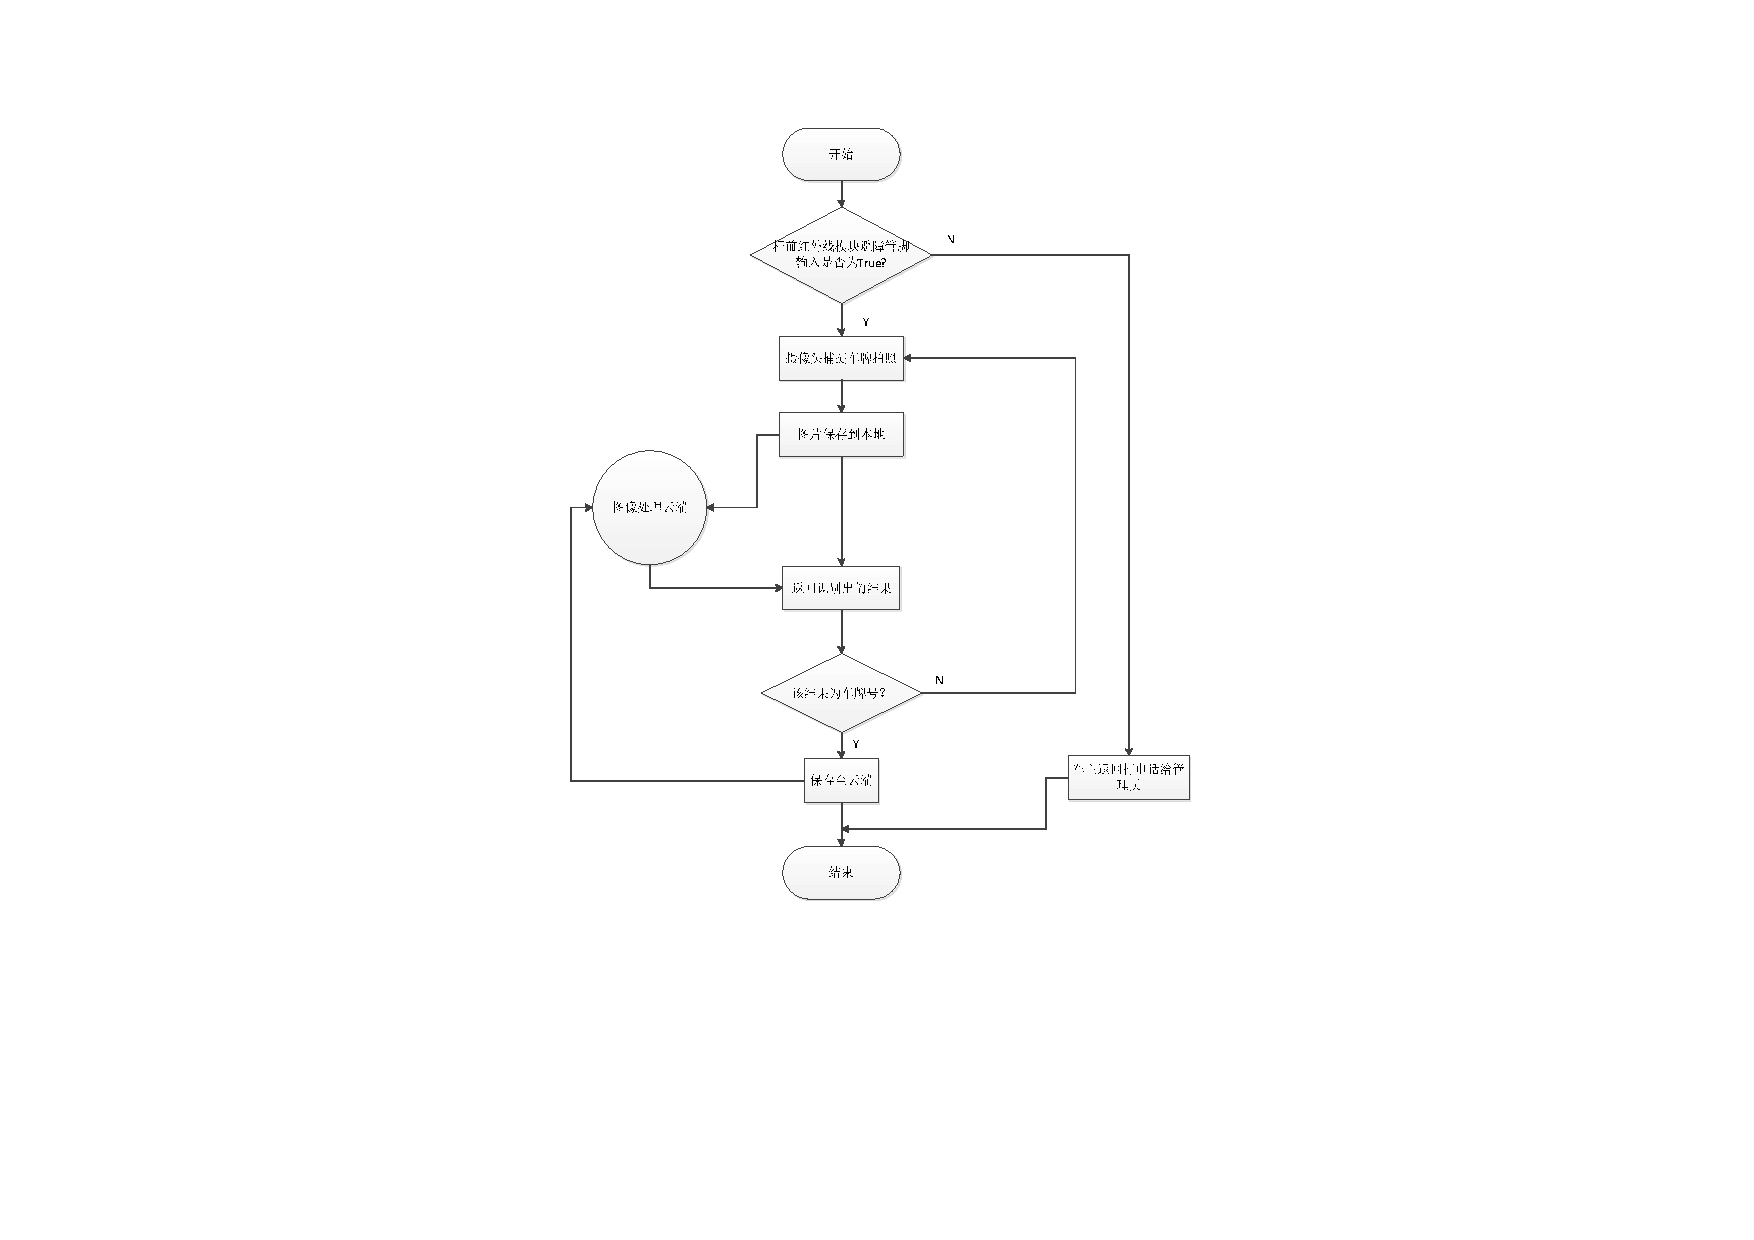
\includegraphics[width=\textwidth]{figure/software-4.pdf}
	\caption{出库拍照模块程序设计流程图}\label{fig:出库拍照模块程序设计流程图}
\end{figure}

\subsubsection{驱动模块的设计}
为了驱动步进电机首先设置主控模块相应的引脚为OutPut模式。主控模块中通过驱动模块带动步进电机旋转,进库时电机起杆(也即电机逆时针旋转90度)。电机在车入库时起杆的最终触发程序是停车管理系统云端显示还有剩余车位,落杆的最终条件是第二个红外模块检测不到车身。入库驱动模块设计流程如图\ref{fig:入库驱动模块设计流程图}所示。

\begin{figure}[htbp]
	\centering
	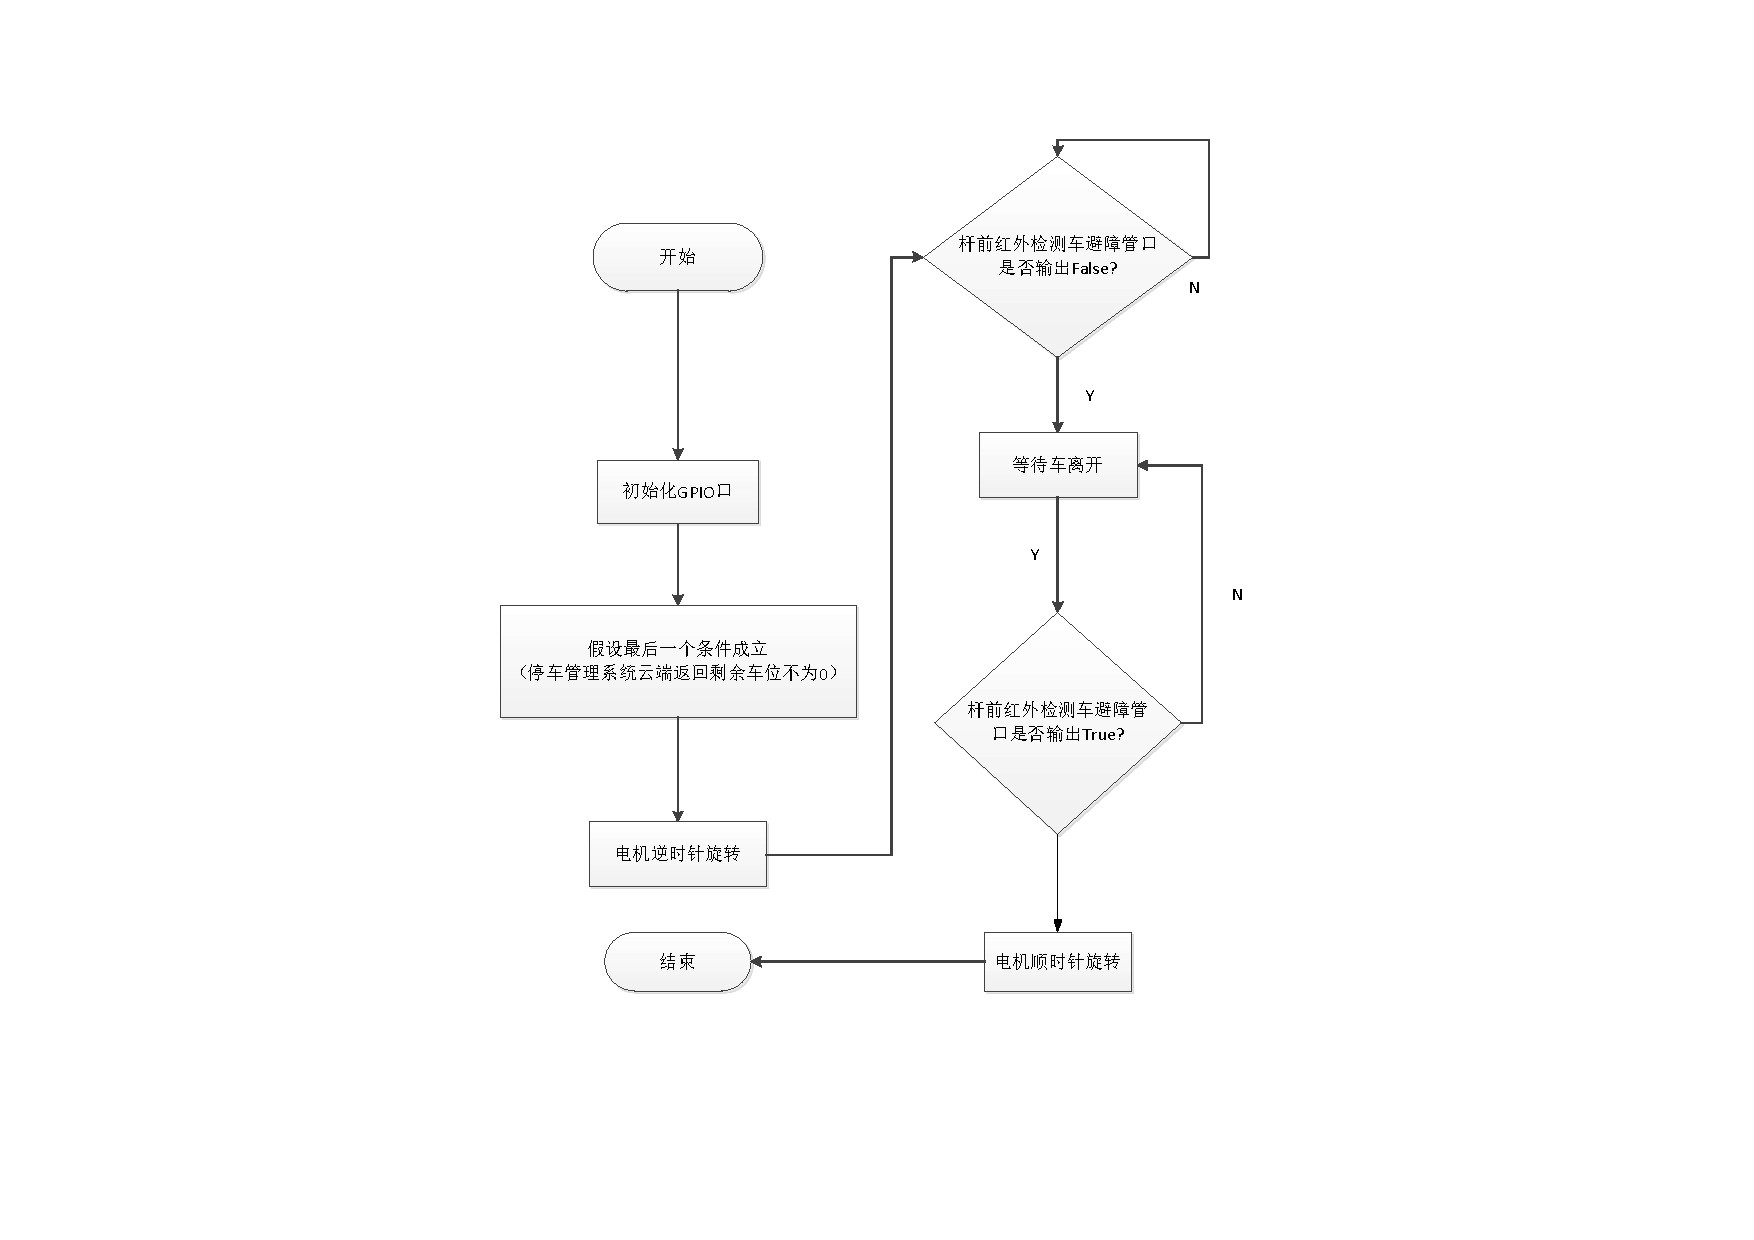
\includegraphics[width=\textwidth]{figure/software-5.pdf}
	\caption{入库驱动模块设计流程图}\label{fig:入库驱动模块设计流程图}
\end{figure}

电机在车出库时起杆的最终条件是车主付款成功,而落杆的最终条件与车入库完全一样。出库驱动模块设计流程图如图\ref{fig:出库驱动模块设计流程图}所示。

\begin{figure}[htbp]
	\centering
	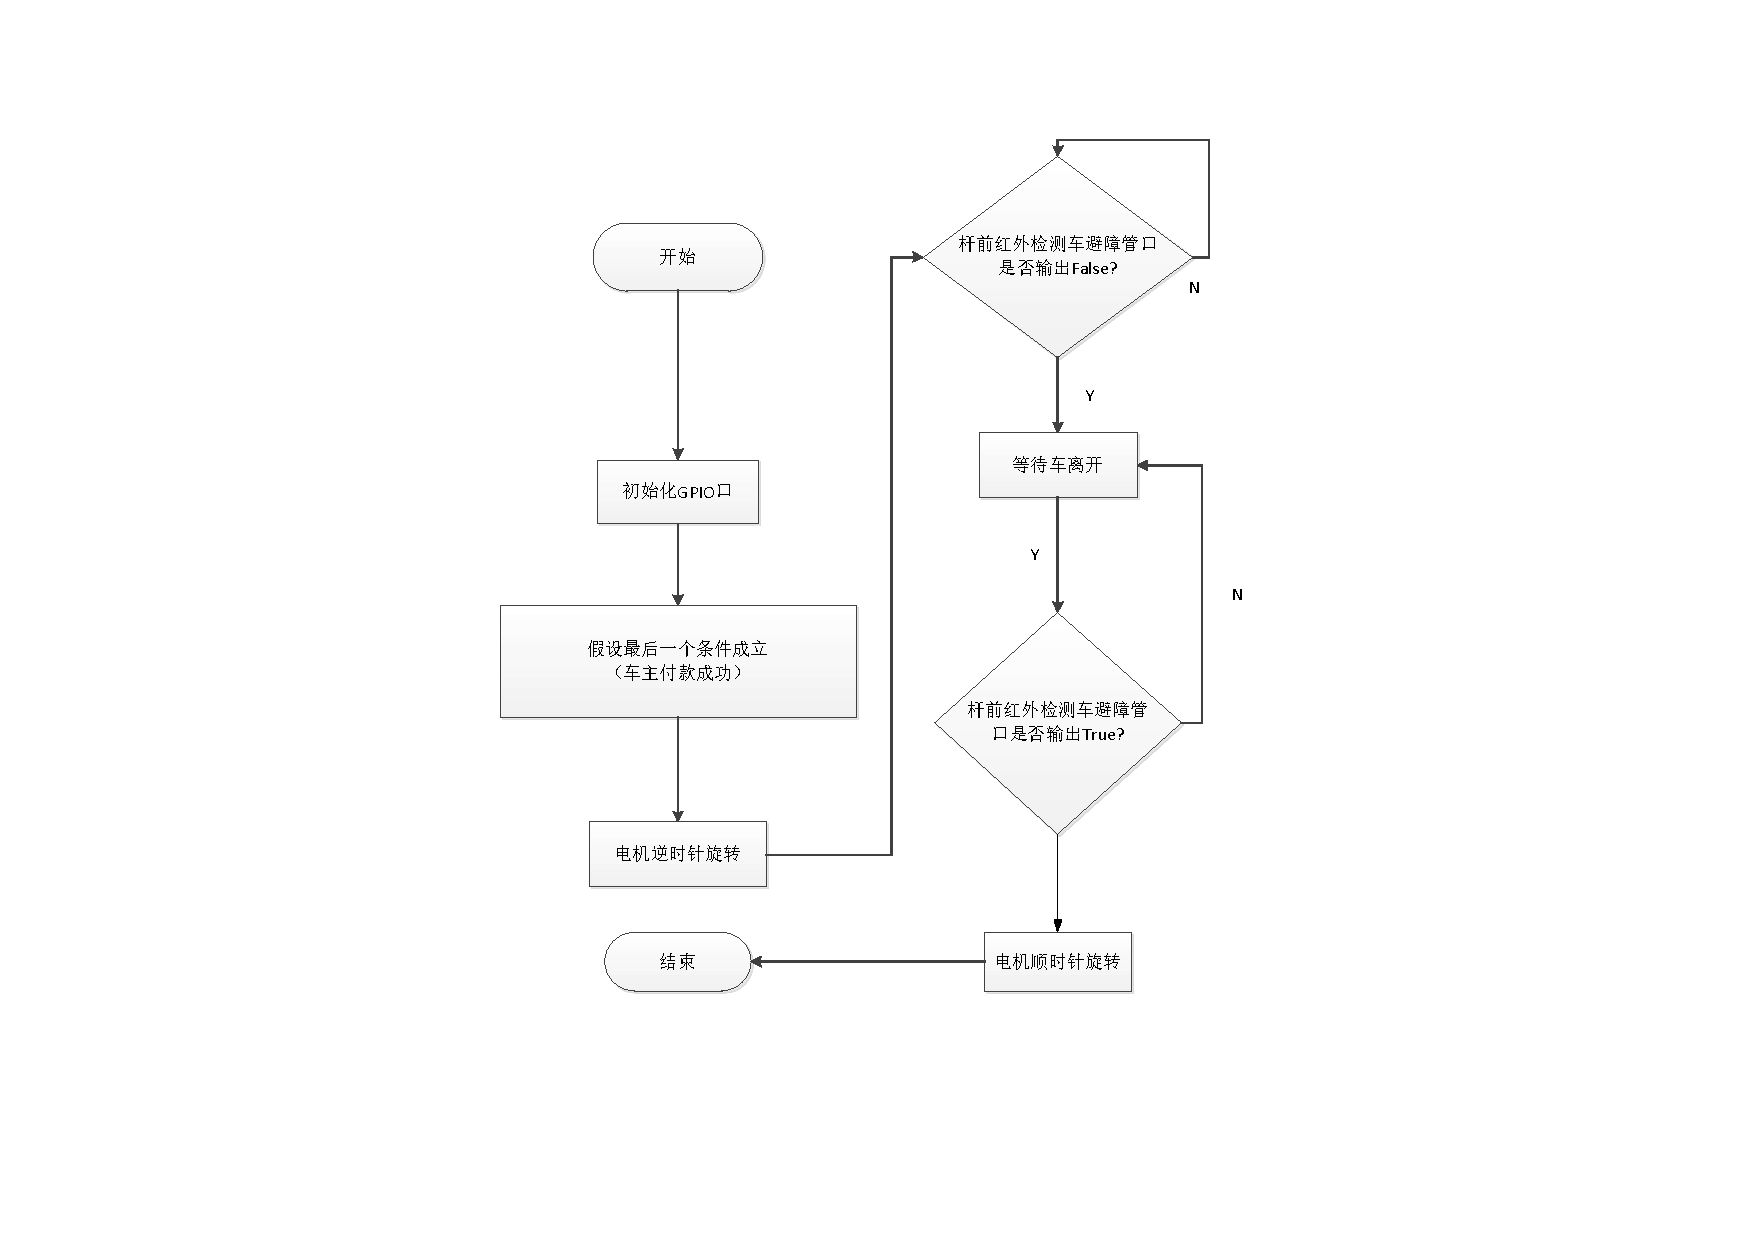
\includegraphics[width=\textwidth]{figure/software-6.pdf}
	\caption{出库驱动模块设计流程图}\label{fig:出库驱动模块设计流程图}
\end{figure}


\subsection{车牌识别算法分析}\label{车牌识别算法分析}
HyperLPR的车牌识别使用的是模板匹配法。该方法对车牌图像要求较高,当车牌倾斜角度很小、边框去除干净、图像噪声较少,字符尺寸和字符间距比较标准时,该算法速度快、分割效果好;而当车牌图像质量较为一般时,该算法的分割效果常常不尽人意。因此在进行车牌识别前需要准确定位图像中的车牌位置,并对车牌字符进行准确分割。

\subsubsection{车牌粗定位}
车牌定位的方法有很多种,在学术界它其实是属于场景文字检测的一种特定情况。
\begin{itemize}
	\item 考虑到字符间垂直边缘比较密集,有基于边缘的方法;
	\item 考虑到字符个体间的特征,有基于个体字符特征的方法;
	\item 考虑到车牌这种共性特征比较强烈的目标 ,有基于目标检测的方法。
\end{itemize}
HyperLPR用了使用了基于目标检测的方法进行车牌粗定位,其使用的目标检测器是基于OpenCV的Haar级联分类器,该分类器使用OpenALPR的Train-Detector进行训练,使用4700张正样本和12000张负样本。正样本通过手动crop或者使用easypr或HyperLPR的crop模块进行裁剪。对于负样本,在train detector目录下已经包含了一些基本的负样本,但是在多次训练后发现,使用这些负样本训练出来的检测器在垂直边缘密集的地方误检特别高,因此改用类似于Hard Sample Mining的策略,将这些部分的误检区域裁剪出来,加入到分类器的训练当中。

使用目标检测器进行粗定位的过程比较简单,在opencv中只需要调用CascadeClassifier进行多尺度检测即可。

\subsubsection{车牌精定位}
HyperLPR使用类似于MSER的方式的多级二值化+RANSAC拟合车牌的上下边界。下面是该过程的大致步骤。
在训练完cascade分类器之后就会,haar adaboost cascade目标检测只能输出三个参数:目标的x 、目标的y 、目标的尺度。

也就是说我们不像DPM和现代目标检测那样可以输出目标的长宽比。所以光凭这三个参数还远远不够,在车牌有角度的倾斜的情况下。与传统目标检测不同的是,HyperLPR更需要确定车牌精确的位置。这里HyperLPR尝试了很多种做法包括直接对ROI区域进行Regression的方法,在少量的测试结果来看并不能取得良好的效果。最后HyperLPR想出了一种较为简单粗暴的精定位算法。

首先为了最大程度的保留车牌图像,对cascade目标检测后的区域进行扩展。在扩展后矩形中做文章。

在完成对cascade目标检测后的区域进行扩展的操作之后,接着使用多个参数对这个区域进行多次自适应二值化,即对opencv中adaptiveThreshold函数的k的参数从选择从-50变化到0。做15次二值化,对每次二值化的图像进行连通域分析寻找满足字符长宽比的轮廓并找出对应的矩形框。将矩形框对角线的两个顶点找出来,进而对下面的点做直线拟合。在做直线拟合之前,这里要特别介绍一下随机抽样一致(RANSAC)算法。

在实际应用中获取到的数据,常常会包含有噪声数据,这些噪声数据会使对模型的构建造成干扰,我们称这样的噪声数据点为outliers,那些对于模型构建起积极作用的我们称它们为inliers,RANSAC做的一件事就是先随机的选取一些点,用这些点去获得一个模型(这个讲得有点玄,如果是在做直线拟合的话,这个所谓的模型其实就是斜率),然后用此模型去测试剩余的点,如果测试的数据点在误差允许的范围内,则将该数据点判为inlier,否则判为outlier。inliers的数目如果达到了某个设定的阈值,则说明此次选取的这些数据点集达到了可以接受的程度,否则继续前面的随机选取点集后所有的步骤,不断重复此过程,直到找到选取的这些数据点集达到了可以接受的程度为止,此时得到的模型便可认为是对数据点的最优模型构建。

由于在做连通域分析的时候,我们仅仅使用满足字符长宽比例boundingbox作为判断条件,所以会带来一定的噪声。RANSAC算法能帮助我们剔除这些噪声点。
使用RANSAC算法对之前找出的点进行拟合,这样就找到了上边界和下边界。

在此基础上使用CNN Regression算法来确定车牌的左右边界。最后只需要对此区域进行裁剪即可。

这样就完成了车牌的精定位。

\subsubsection{车牌倾斜校正}
目前稳定可靠的文字倾斜检测主要有Radon 变换和 Hough 变换两种,不过这两种算法的时间复杂度都在$O(n^3)$级别。这种方法往往需要大量数值运算,在文字大量出现的图片显得效率低下力不从心。

因此HyperLPR使用了基于方向纹理场的算法进行车牌校正倾斜。该算法是受lsd直线检测算法的启发,发现可以统计各个方向场的角度来寻找图像中纹理最为密集的两个方向。主要计算公式如公式(\ref{eq:HyperLPR}),其运行步骤如下:
\begin{enumerate}
	\item 将图像划分为不重叠的子块(16×16);
	\item 利用Sobel算子计算每个子块像素点的梯度值;
	\item 利用公式(\ref{eq:HyperLPR})计算中心点在$(i,j)$的子块的脊线的方向;
	\item 以$(1/\pi)$为bin统计各个块方向的直方图;
	\item 使用高斯滤波进行核密度的估计(平滑);
	\item 选取在两个区间的极大值作为校正方向。
\end{enumerate}

\begin{equation}\label{eq:HyperLPR}
	\begin{split}
		V_x(i,j)&=\sum_{u=i-w/2}^{i+w/2}\sum_{v=j-w/2}^{j+w/2}2\partial_x(u,v)\partial_y(u,v)\\
		V_y(i,j)&=\sum_{u=i-w/2}^{i+w/2}\sum_{v=j-w/2}^{j+w/2}\partial^2_x(u,v)\partial^2_y(u,v)\\
		\theta(i,j)&=\frac{1}{2}tan^{-1}(\frac{V_y(i,j)}{V_x(i,j)})
	\end{split}
\end{equation}

\subsubsection{字符识别}
模板匹配法根据车牌的标准样式,结合字符的结构、尺寸和间距特征,设计出一个固定的模板和一个用来度量模板匹配程度的评价函数,然后将该模板在归一化后的图像中从左至右滑动,每滑动一次计算对应的评价值,最终选出匹配程度最高的模板滑动位置作为字符分割的位置,并以此模板对应的字符作为当前位置的字符识别结果。


\subsection{云服务设计}\label{云服务设计}
云端服务要实现的功能主要有4个:数据存储、车牌识别、道闸控制和付款管理。这4个功能分别由4个微服务完成,它们之间的关系如图\ref{fig:云端微服务关系结构图}所示。

\begin{figure}[htbp]
	\centering
	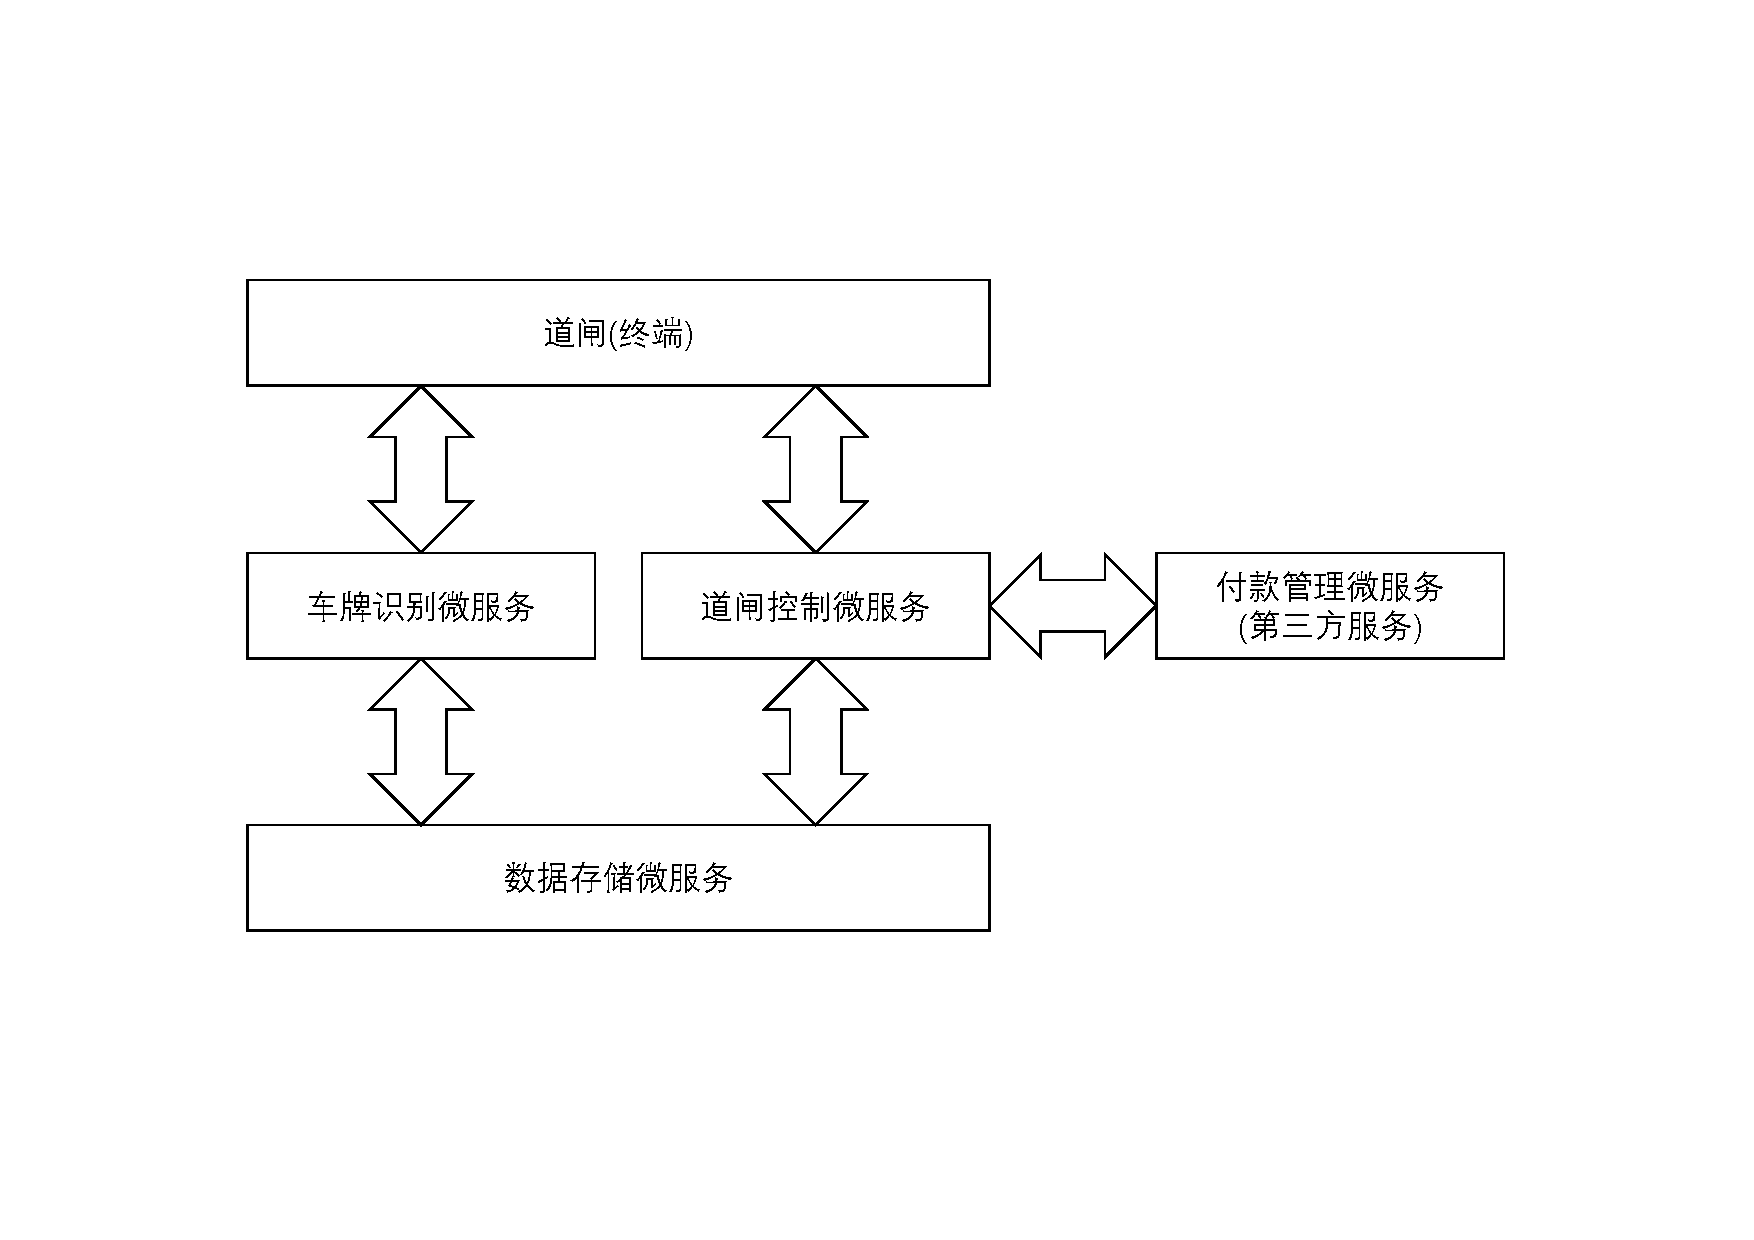
\includegraphics[width=\textwidth]{figure/server-all.pdf}
	\caption{云端微服务关系结构图}\label{fig:云端微服务关系结构图}
\end{figure}

\subsubsection{数据存储微服务}
数据存储是整个云服务系统的基础,它承担着记录车牌识别和车辆出入情况,并为客户端和云服务系统的快速即时通信提供可靠的数据支持。数据存储微服务的组成部分和各自的特性功能如下:
\begin{itemize}
	\item 关系型硬盘数据库:提供可靠而大容量的数据存储,但速度较慢,用于存储历史记录;
	\item 非关系型内存数据库:提供快速小容量的数据存储,用于存储需要经常访问的运行数据;
	\item 文件系统:用于存储图片等不便于进入数据库的文件数据。
\end{itemize}

\subsubsection{车牌识别微服务}
由于树莓派操作系统的特殊性,道闸终端上无法稳定运行通常的图像识别库,因此需要将\ref{车牌识别算法分析}中所介绍的车牌识别算法封装为一个车牌识别微服务部署在云端,该微服务将接收并识别道闸终端拍照上传的车牌图像,并将识别结果发回到道闸终端,从而使道闸具备车牌识别功能。车牌识别微服务的运行流程如图\ref{fig:车牌识别微服务运行流程}。

\begin{figure}[htbp]
	\centering
	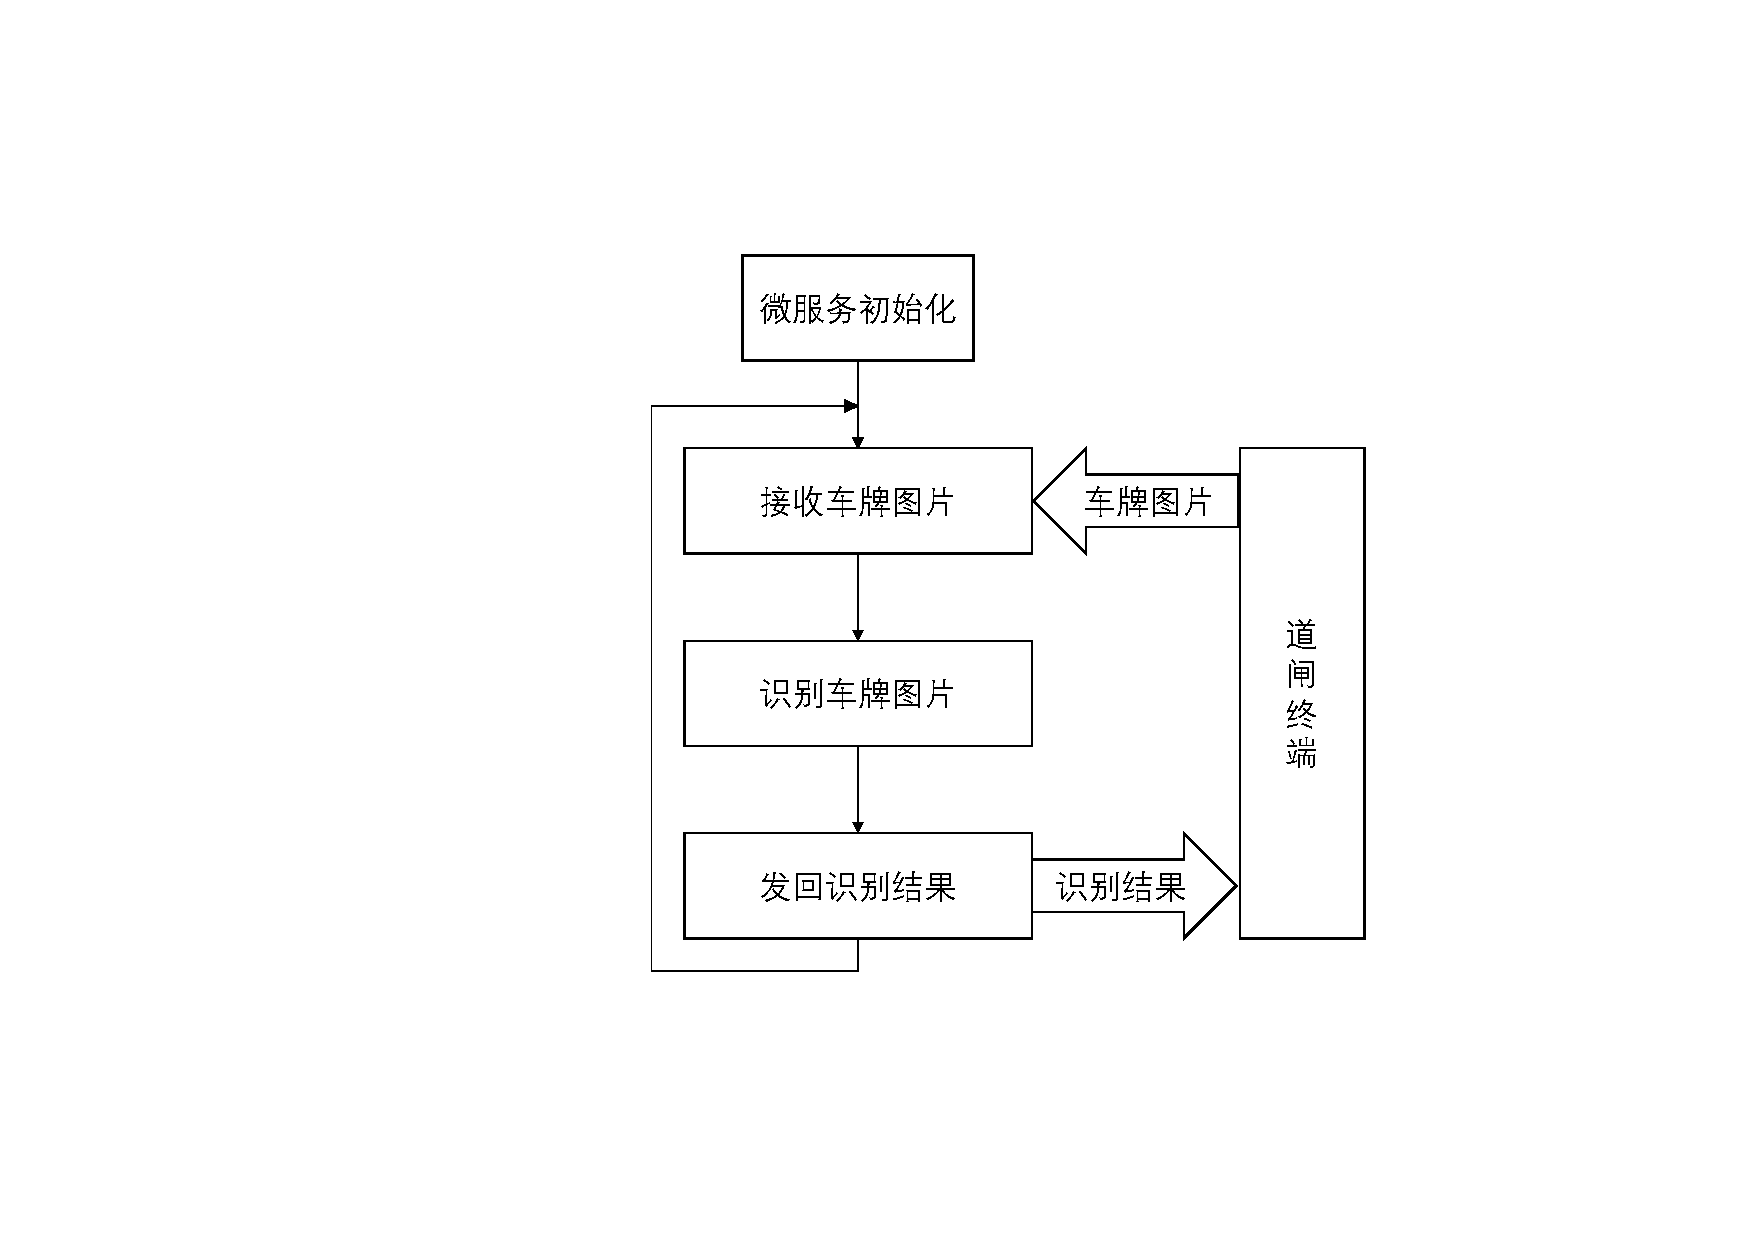
\includegraphics[width=\textwidth]{figure/server-python.pdf}
	\caption{车牌识别微服务运行流程}\label{fig:车牌识别微服务运行流程}
\end{figure}

\subsubsection{道闸控制微服务}\label{道闸控制微服务}
道闸控制微服务是整个云服务系统的核心,也是系统中功能部件最多、结构最为复杂的微服务。道闸控制微服务的功能可分为以下三类:
\begin{itemize}
	\item 接收处理道闸终端上传的车辆信息,并返回开关指令控制道闸的放行;
	\item 与第三方付款管理服务通信,实现出口处的计时收费功能;
	\item 与管理员客户端通信,实时同步车辆信息和历史记录。
\end{itemize}

其主要运行流程如下:

\begin{enumerate}[label=\bf{\arabic*、}]
	\item {\bf 控制入口道闸}

	      在入口处,道闸终端在检到车辆并识别出车牌号后,会向服务器发送一条包含车牌号的进入信息,这时服务器需要判断停车场内是否还有剩余车位,若有则向终端返回“放行”指令并在历史记录数据库和运行数据库中记录下车辆的进入时间,否则返回“不放行”指令。其流程图如图\ref{fig:入口道闸控制运行流程}。

	      \begin{figure}[htbp]
		      \centering
		      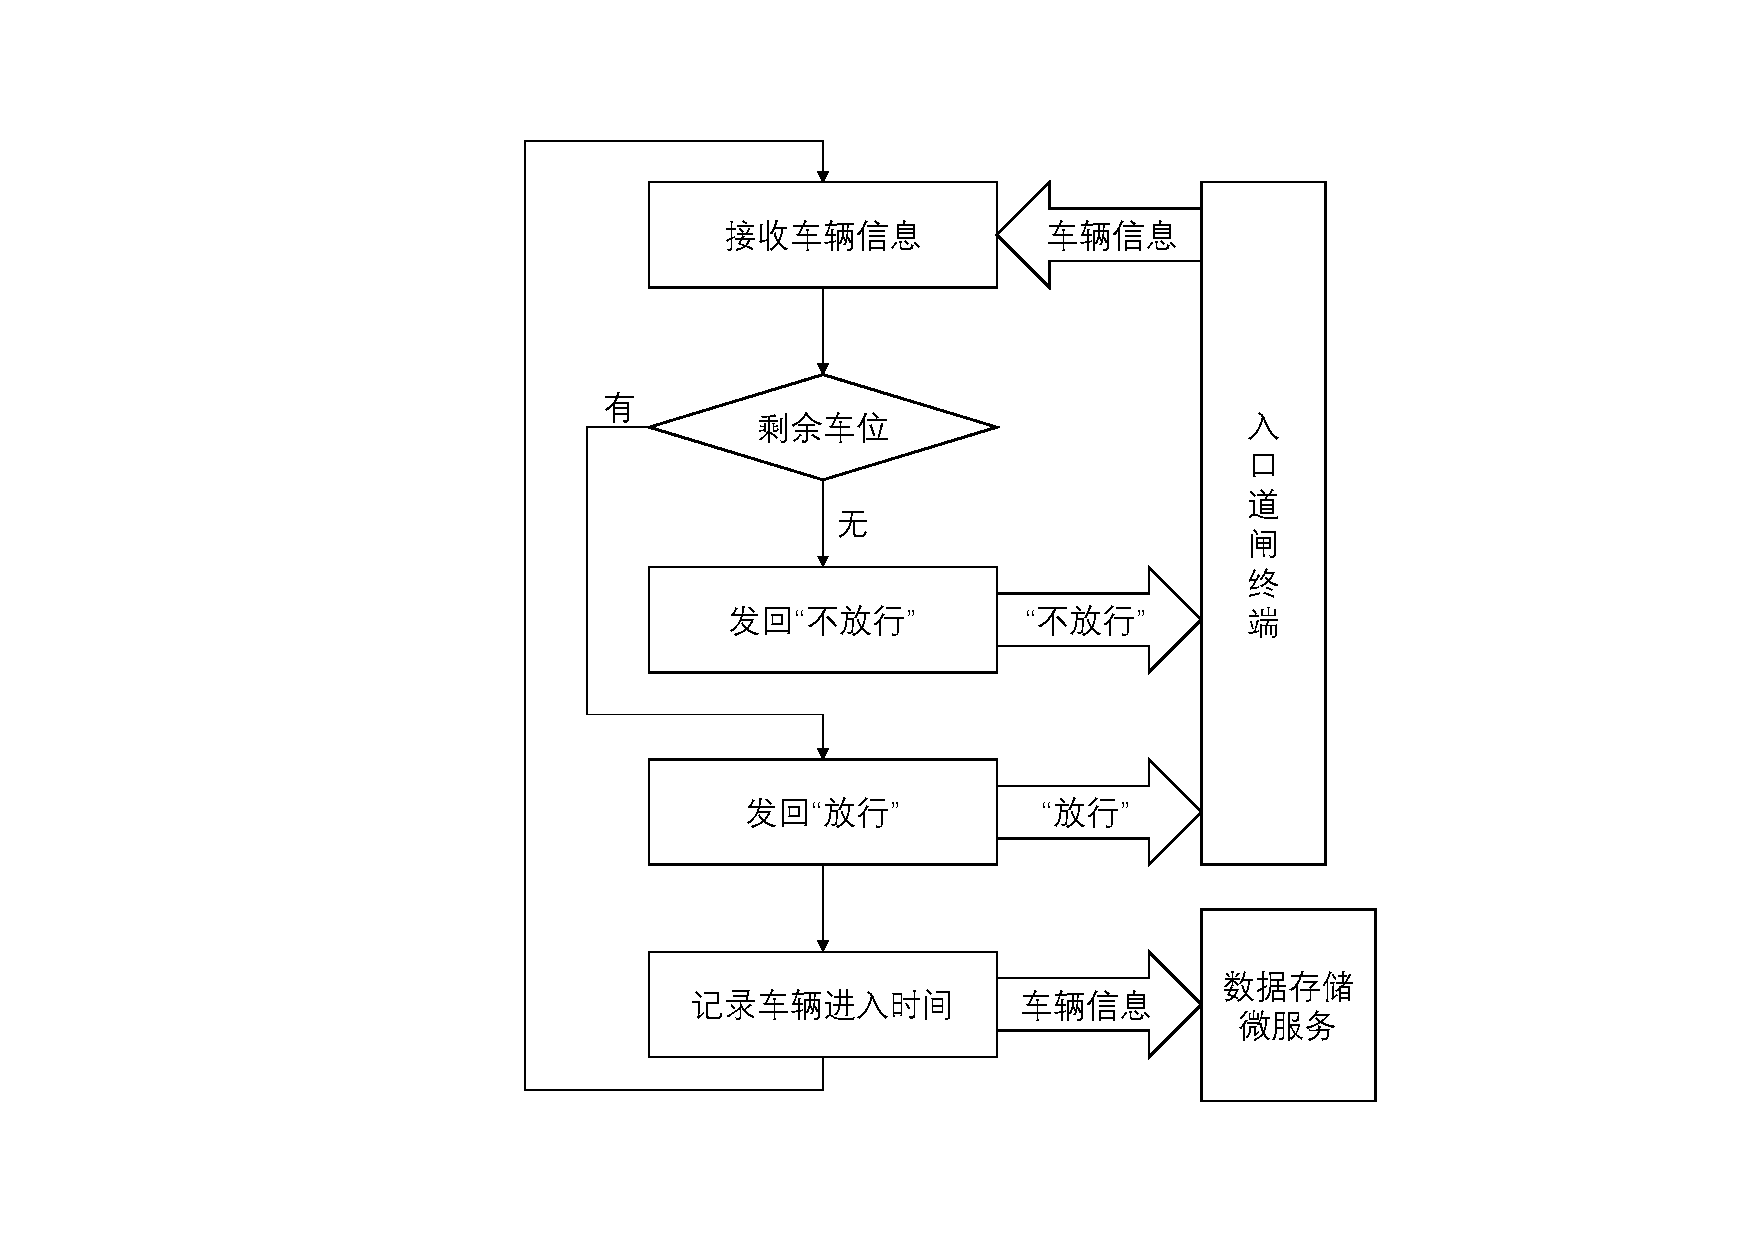
\includegraphics[width=\textwidth]{figure/server-enter.pdf}
		      \caption{入口道闸控制服务运行流程}\label{fig:入口道闸控制运行流程}
	      \end{figure}

	\item {\bf 控制出口道闸}

	      在入口处类似处,出口道闸终端也会在检测到车辆并识别出车牌号后向服务器发送一条包含车牌号的信息,这时服务器需要进行如下操作:
	      \begin{enumerate}[label=\arabic*、]
		      \item 从数据库中获取到该车的进入时间;
		      \item 获取当前时间,计算时间差和应付金额;
		      \item 在付款管理服务中创建一个付款订单,并获取到订单信息;
		      \item 向终端发回订单信息;
		      \item 向付款管理服务轮询订单支付状态,直到订单支付完成或被取消;
		      \item 若订单支付完成,则向终端发回“放行”指令,否则发回“不放行”指令;
		      \item 在数据存储微服务中写入付款记录。
	      \end{enumerate}

	      其流程图如图\ref{fig:出口道闸控制运行流程}所示。

	      \begin{figure}[htbp]
		      \centering
		      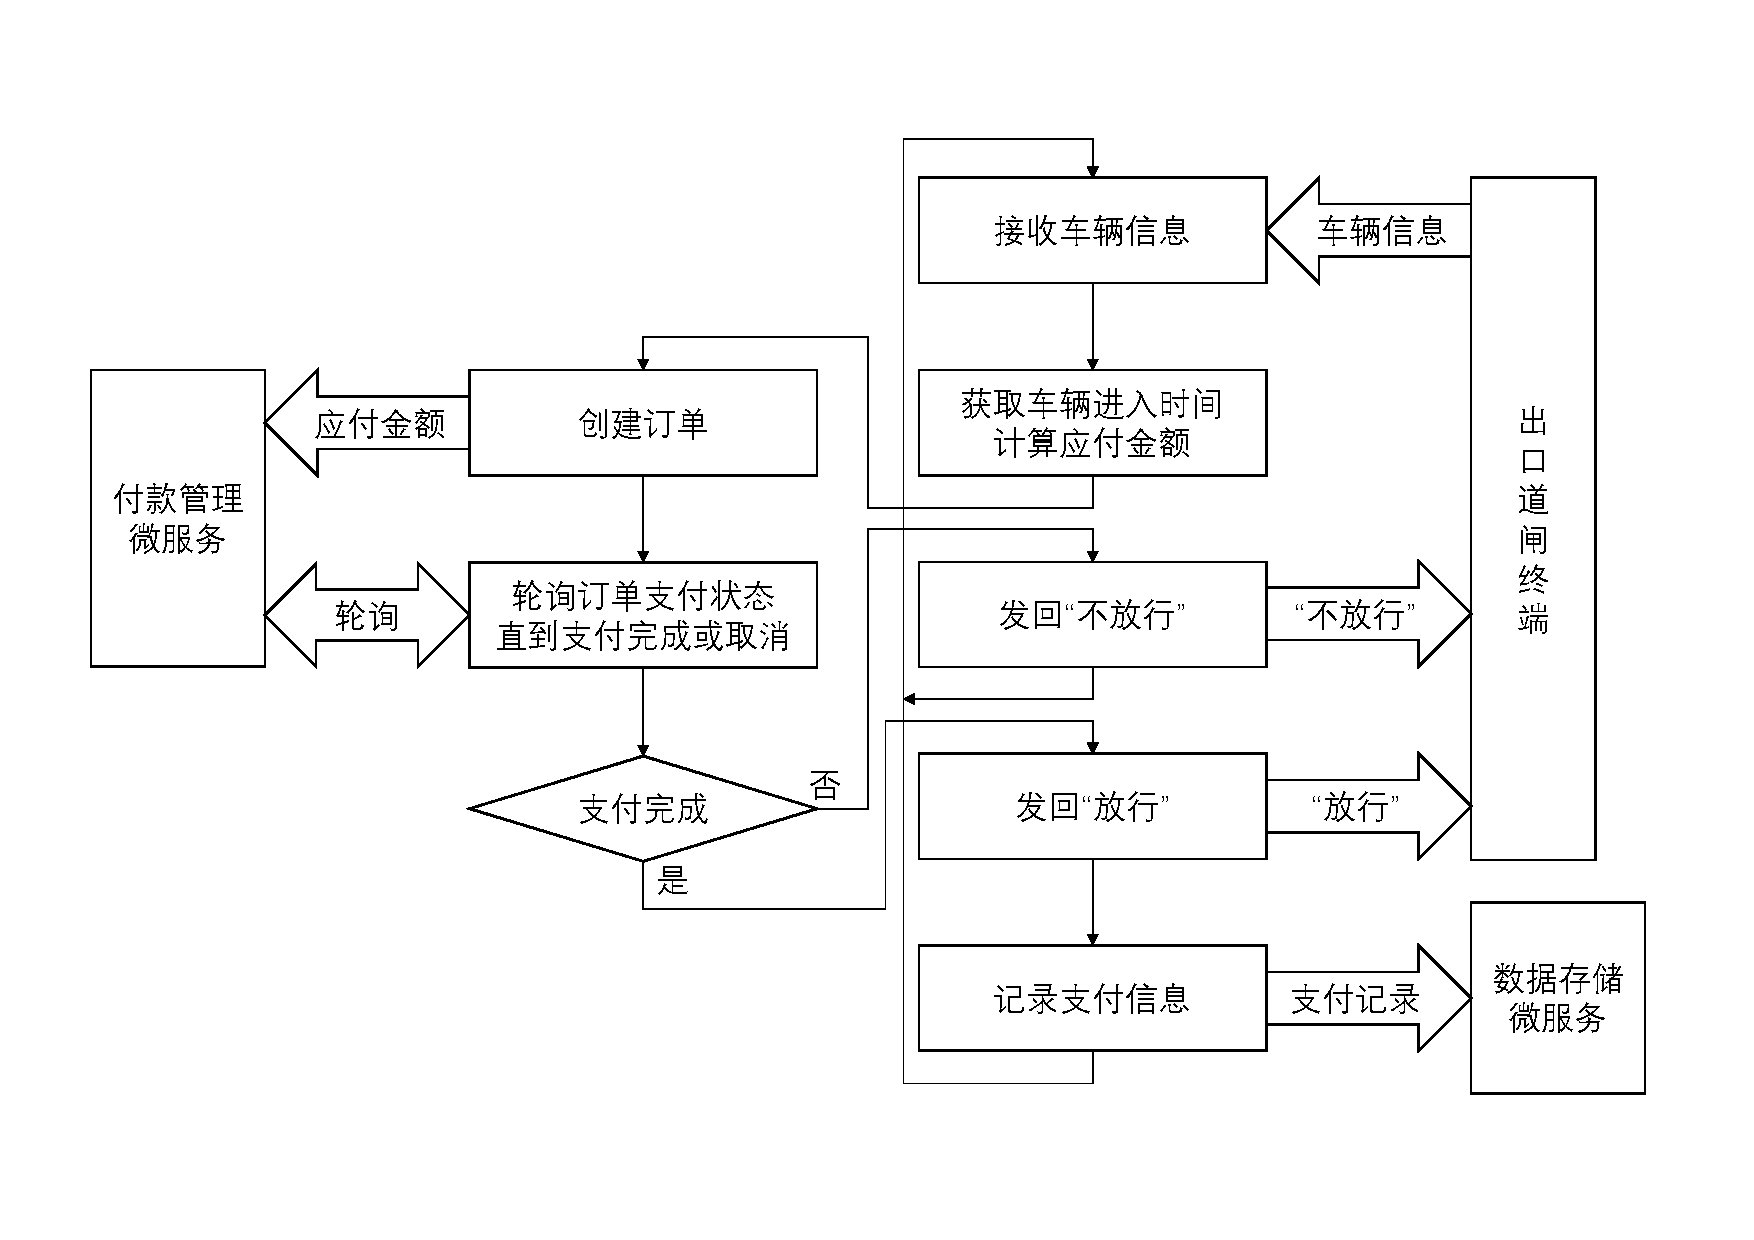
\includegraphics[width=\textwidth]{figure/server-exit.pdf}
		      \caption{出口道闸控制服务运行流程}\label{fig:出口道闸控制运行流程}
	      \end{figure}

	\item {\bf 支持客户端网页上停车情况的即时更新}

	      客户端网页的即时更新由一个位于数据存储微服务中的数据刷新标志位所控制。每当系统中写入了新的车辆出入和付款记录时,这个标志位就会置1,这时服务器会经由与客户端之间建立的长轮询向客户端发送“更新数据”的指令;客户端接到“更新数据”的指令后,再以普通HTTP请求方式获取到新的服务器数据,并刷新页面显示。其流程图如图\ref{fig:客户端网页即时更新服务运行流程}所示。

	      \begin{figure}[htbp]
		      \centering
		      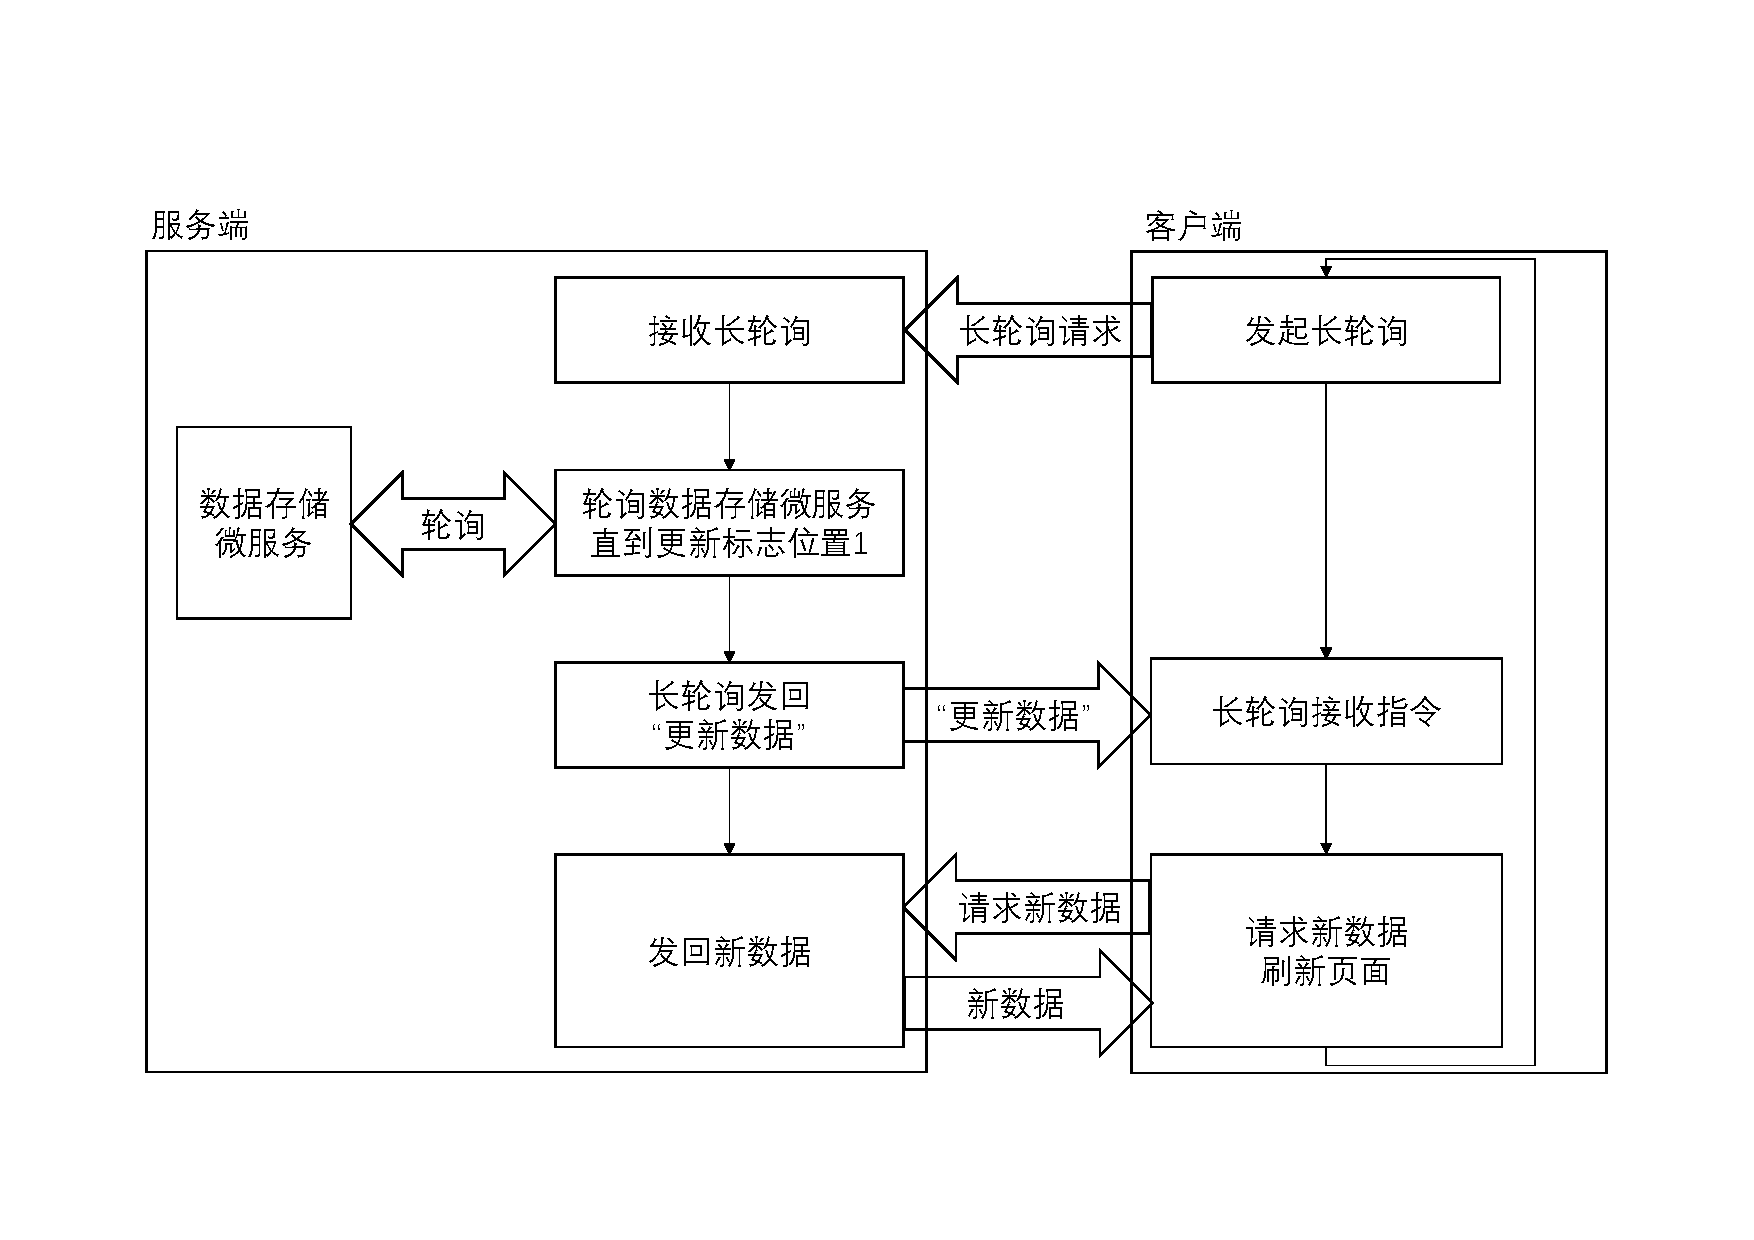
\includegraphics[width=\textwidth]{figure/server-client.pdf}
		      \caption{客户端网页即时更新服务运行流程}\label{fig:客户端网页即时更新服务运行流程}
	      \end{figure}

	\item {\bf 获取道闸放行历史记录}

	      网页客户端中除即时更新显示当前停车场内车辆情况外,还需要显示历史记录。和当前车辆情况显示不同,显示历史记录并不要求实时性,因此可以使用简单的HTTP请求方式从服务器端获取。其流程图如图\ref{fig:客户端获取历史记录流程}所示。

	      \begin{figure}[htbp]
		      \centering
		      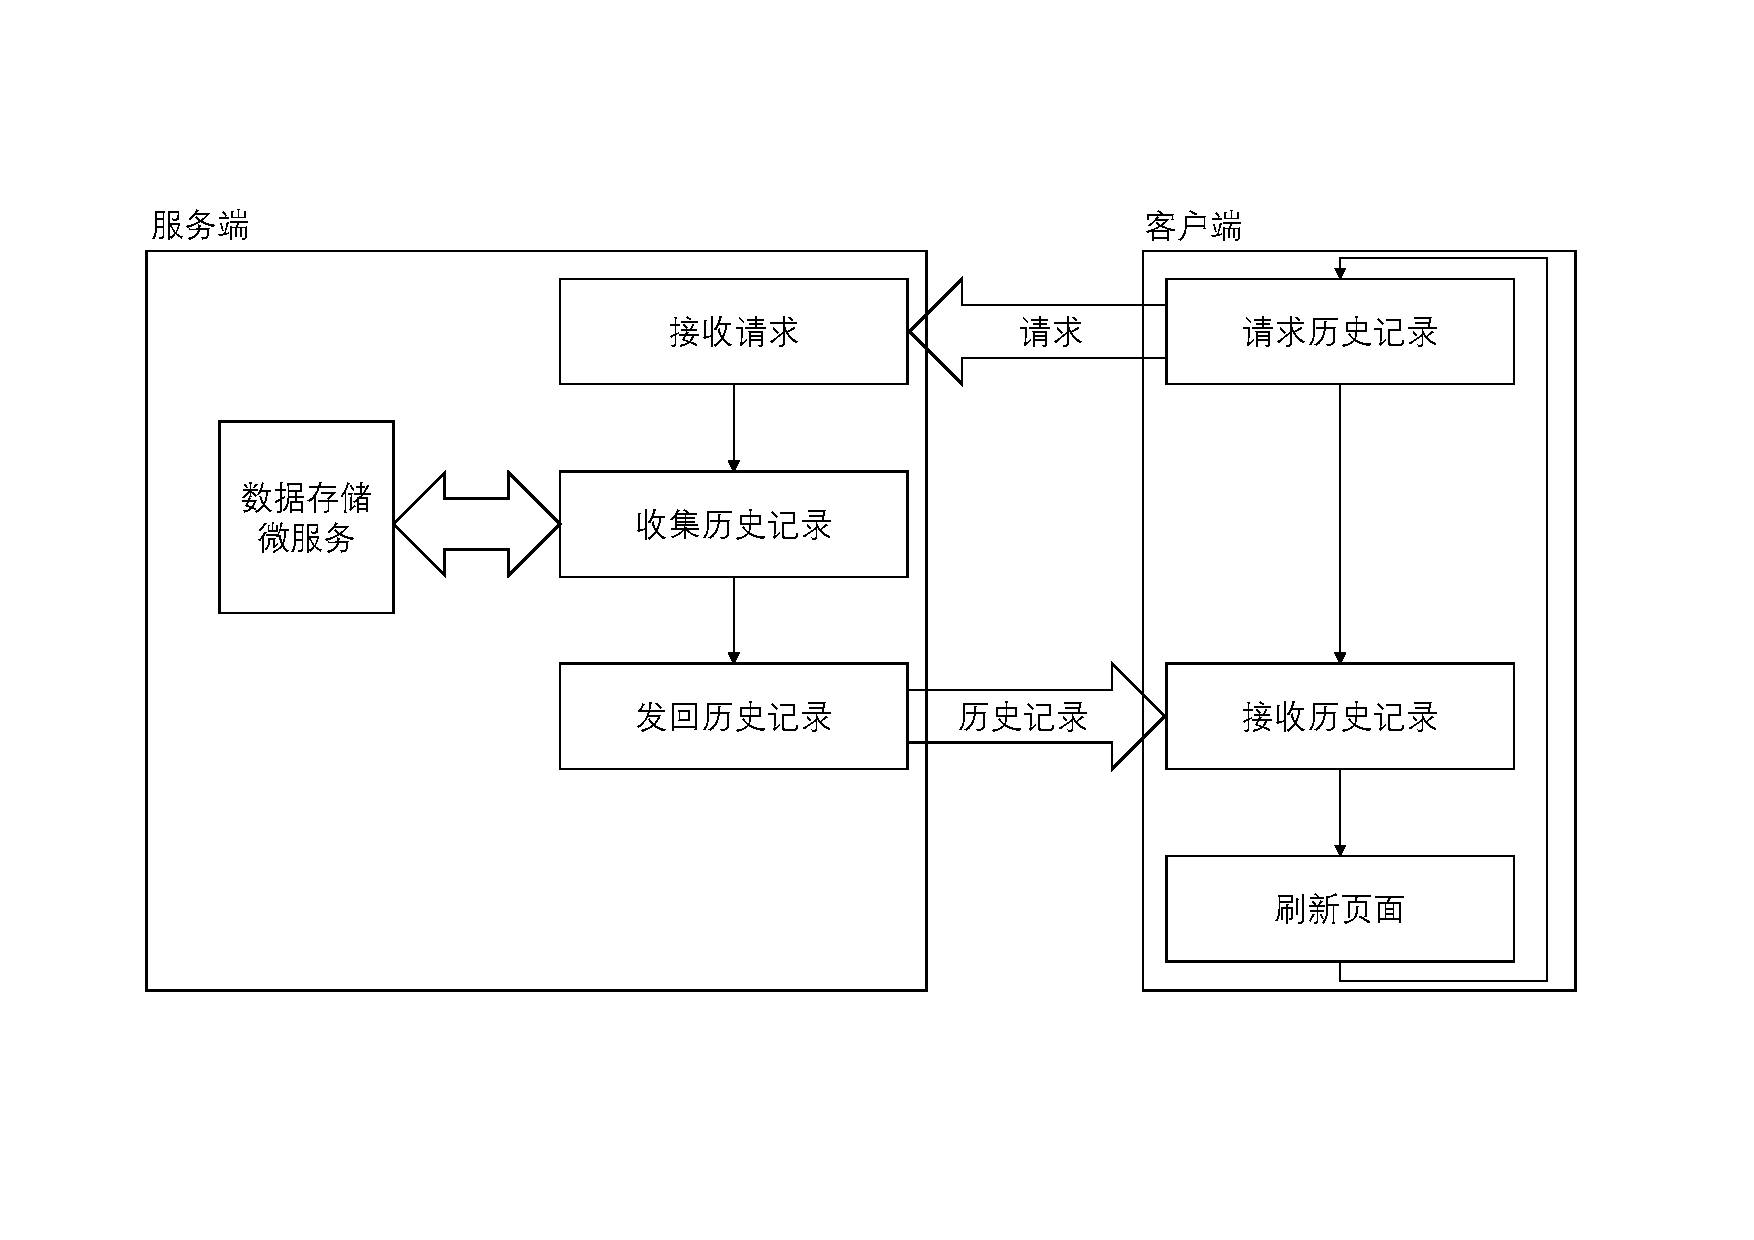
\includegraphics[width=\textwidth]{figure/server-history.pdf}
		      \caption{客户端获取历史记录流程}\label{fig:客户端获取历史记录流程}
	      \end{figure}
\end{enumerate}

\subsubsection{付款管理微服务}\label{付款管理微服务}
由于目前大多数第三方付款管理服务都需要注册经营执照,无法在项目中使用,因此本项目仿照支付宝标准付款接口在微服务架构中添加了一个模拟的第三方支付管理微服务,该微服务被设计为不与本项目中的其他任何微服务有依赖关系,从而能最大程度地模拟第三方付款管理服务的运行。支付宝标准付款接口的运行可以简化为如图\ref{fig:付款管理服务运行流程}所示的流程。

\begin{figure}[htbp]
	\centering
	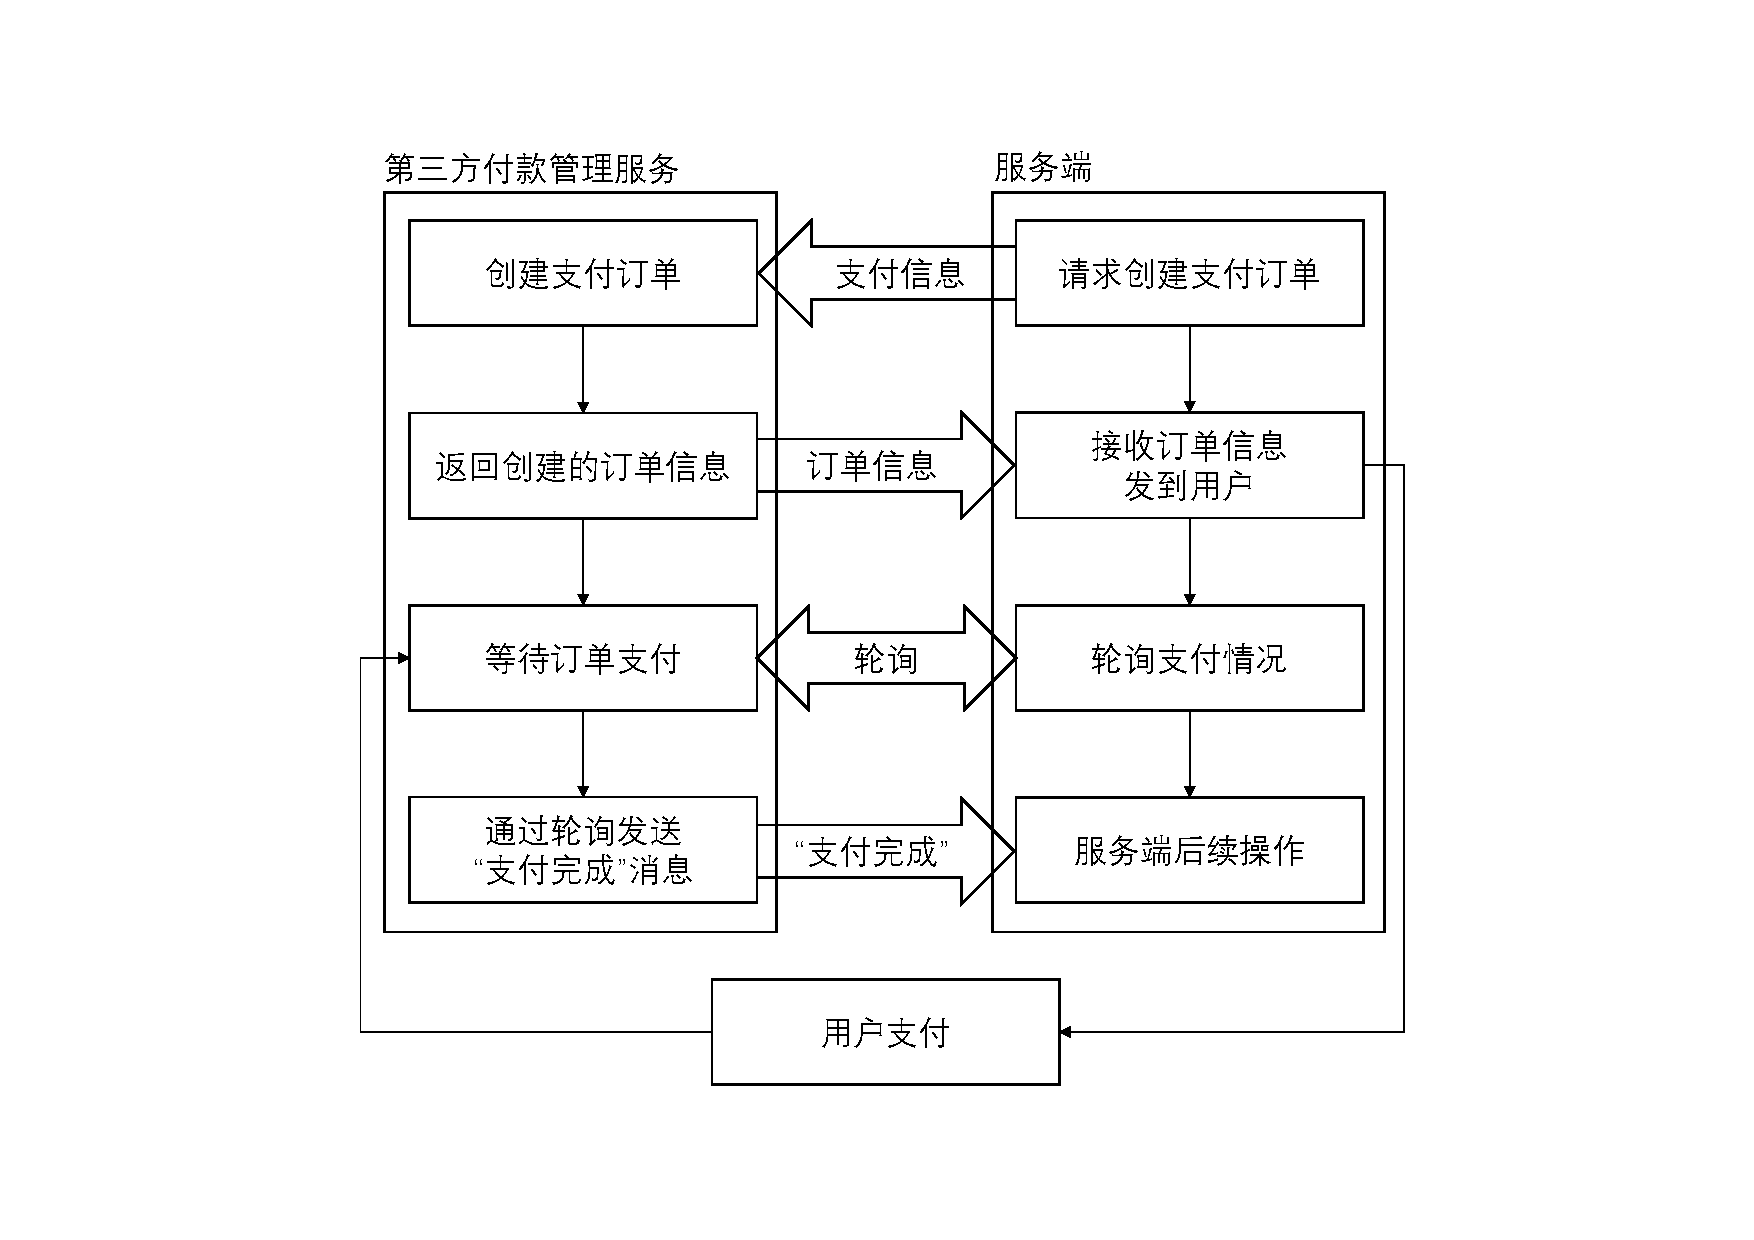
\includegraphics[width=\textwidth]{figure/server-alipay.pdf}
	\caption{付款管理服务运行流程}\label{fig:付款管理服务运行流程}
\end{figure}

\section{系统实现}
\subsection{道闸硬件实现}
前文已经介绍了系统的总体设计和相关算法算法,本节将结合前文,具体实现一个基于树莓派和云服务的停车场道闸系统的硬件搭建。

系统硬件搭建主要是将个子模块通过GPIO口和CSI(摄像机串行接口)连接到树莓派上。其中摄像机连接CSI接口,只要注意方向插入即可;用来感应是否有车到来的红外传感器除了接VCC和GND外,电平输出端接树莓派的GPIO 21(Pin 40);用来感应车辆是否通过道闸的红外传感器除了接VCC和GND外,电平输出端接树莓派的GPIO 20(Pin 38);步进电机驱动芯片上IN1~4四个接口分别接树莓派的GPIO 5(Pin 29),GPIO 6(Pin 31),GPIO 13(Pin 33),GPIO 19(Pin 35)。

硬件接线如图\ref{fig:硬件接线图}所示,最终完成实物如图\ref{fig:系统硬件实物图}。

\begin{figure}[htbp]
	\centering
	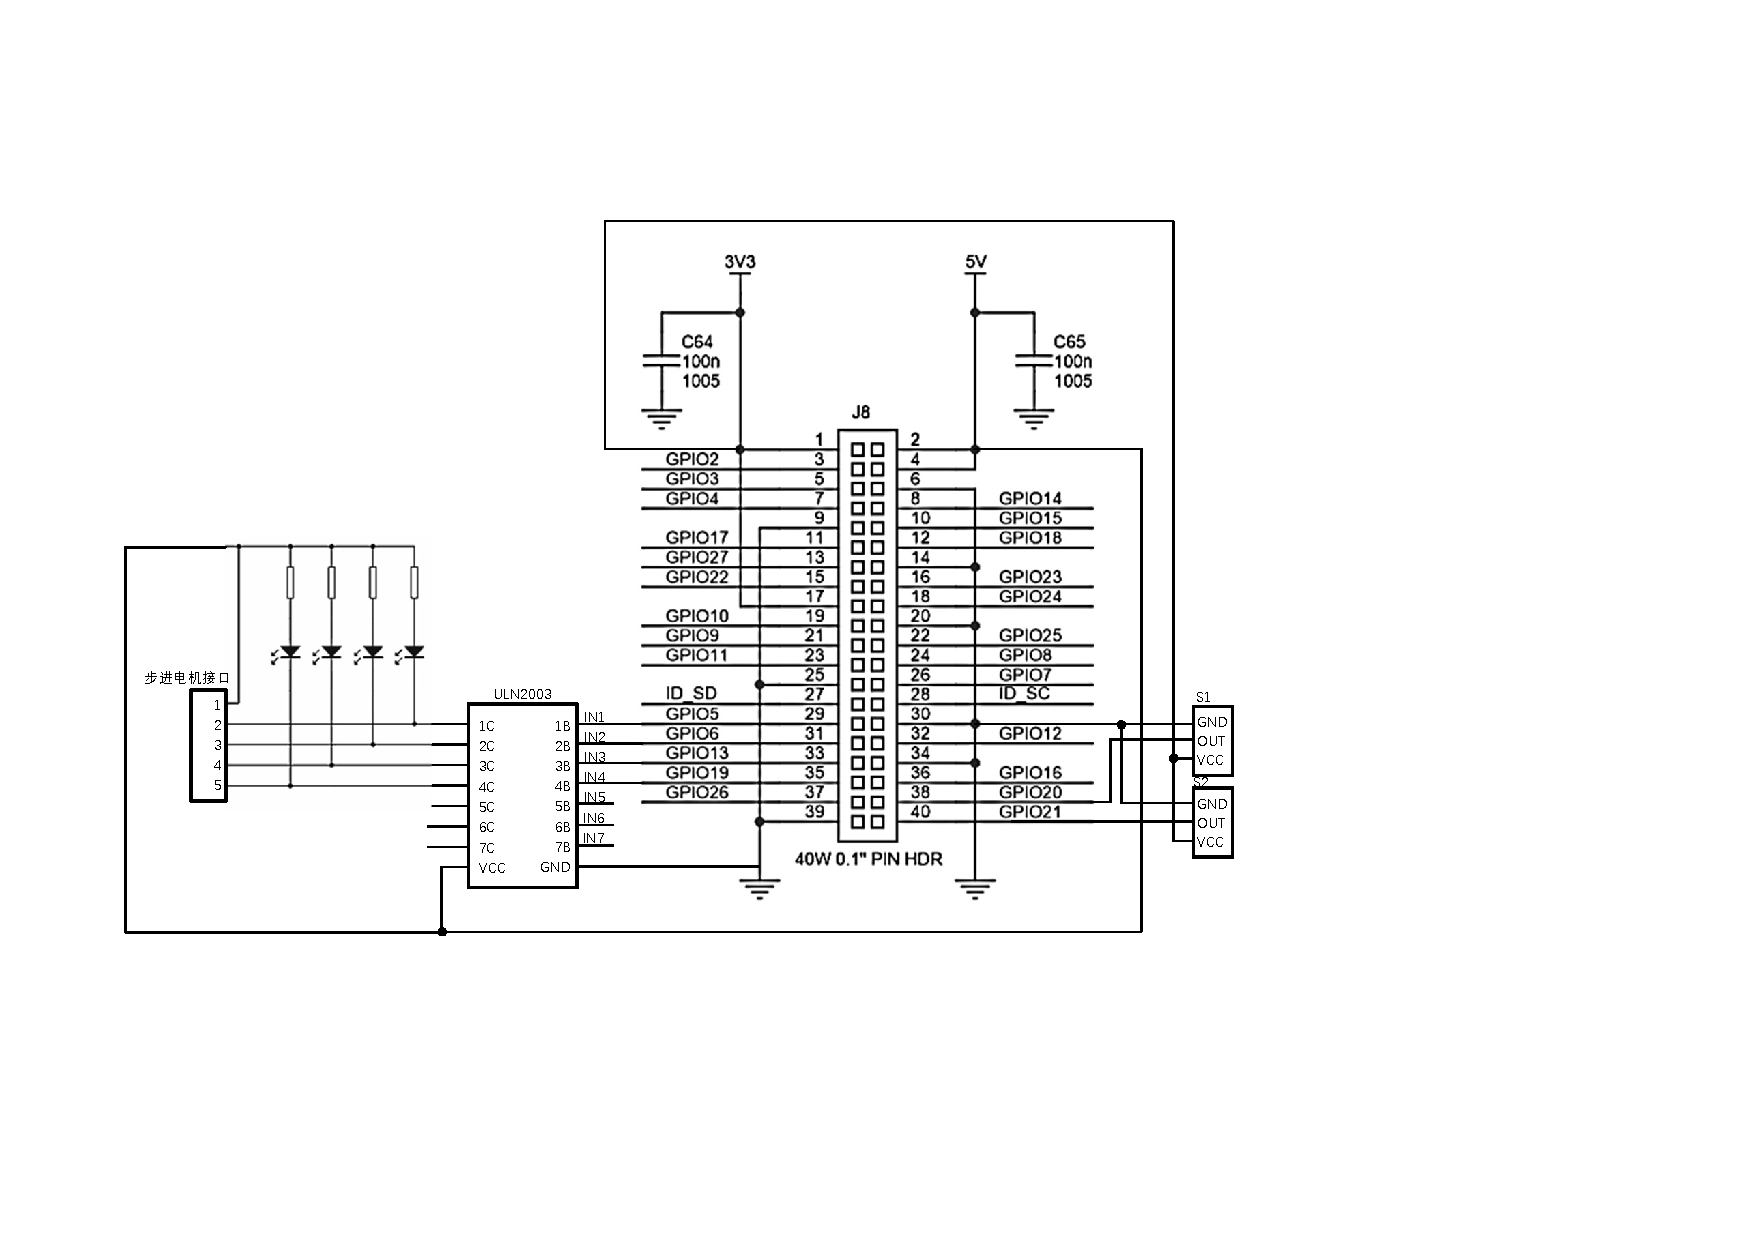
\includegraphics[width=\textwidth]{figure/archive-pin.pdf}
	\caption{硬件接线图}\label{fig:硬件接线图}
\end{figure}

\begin{figure}[htbp]
	\centering
	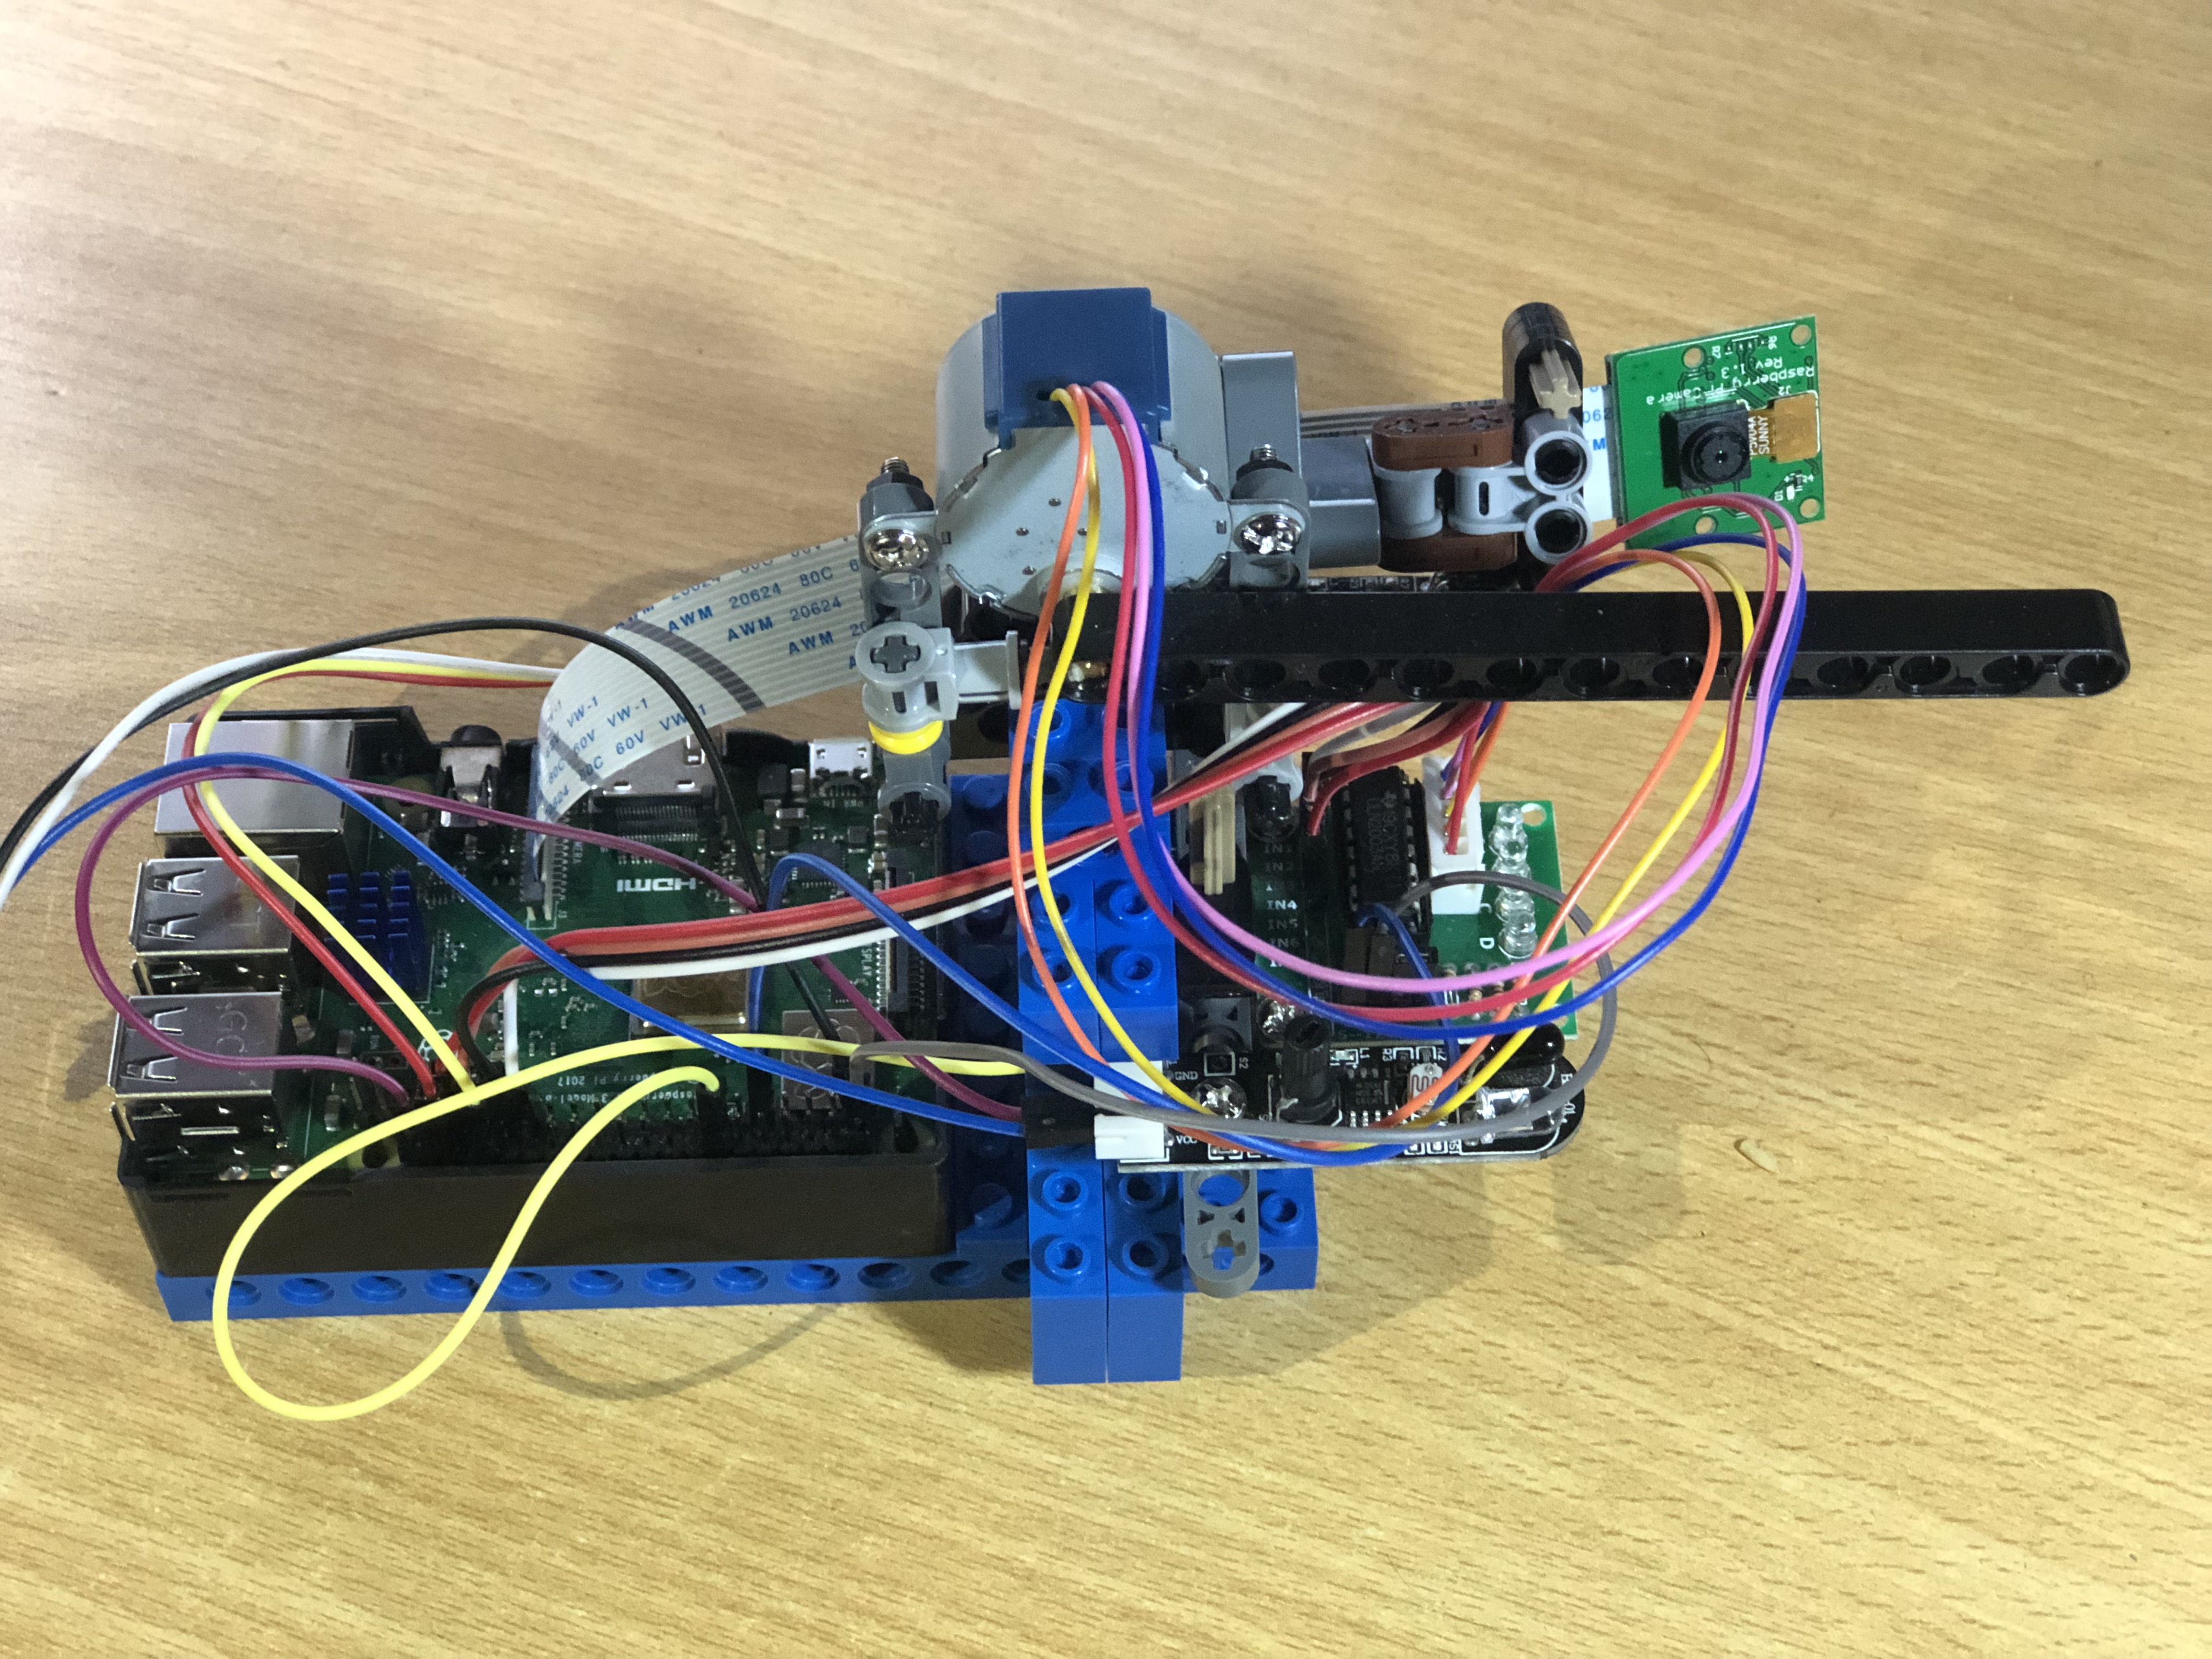
\includegraphics[width=\textwidth]{figure/archive.JPG}
	\caption{系统硬件实物图}\label{fig:系统硬件实物图}
\end{figure}

\subsection{道闸软件实现}
前文已经介绍了系统总体设计(包含硬件设计及软件设计)和相关算法。本
小节将结合前文,具体实现一个停车管理系统。本系统以树莓派3b+为硬件平台利用python为编译环境实现。另外也设计了两个云端服务器:其中一个是车牌识别云端服务器,用来将树莓派摄像头拍下的照片进行处理得出车牌号码;另外一个是停车管理系统云端服务器,用来管理车辆。实现流程图如图\ref{fig:进出库总体任务分析流程图}所示。

\begin{figure}[htbp]
	\centering
	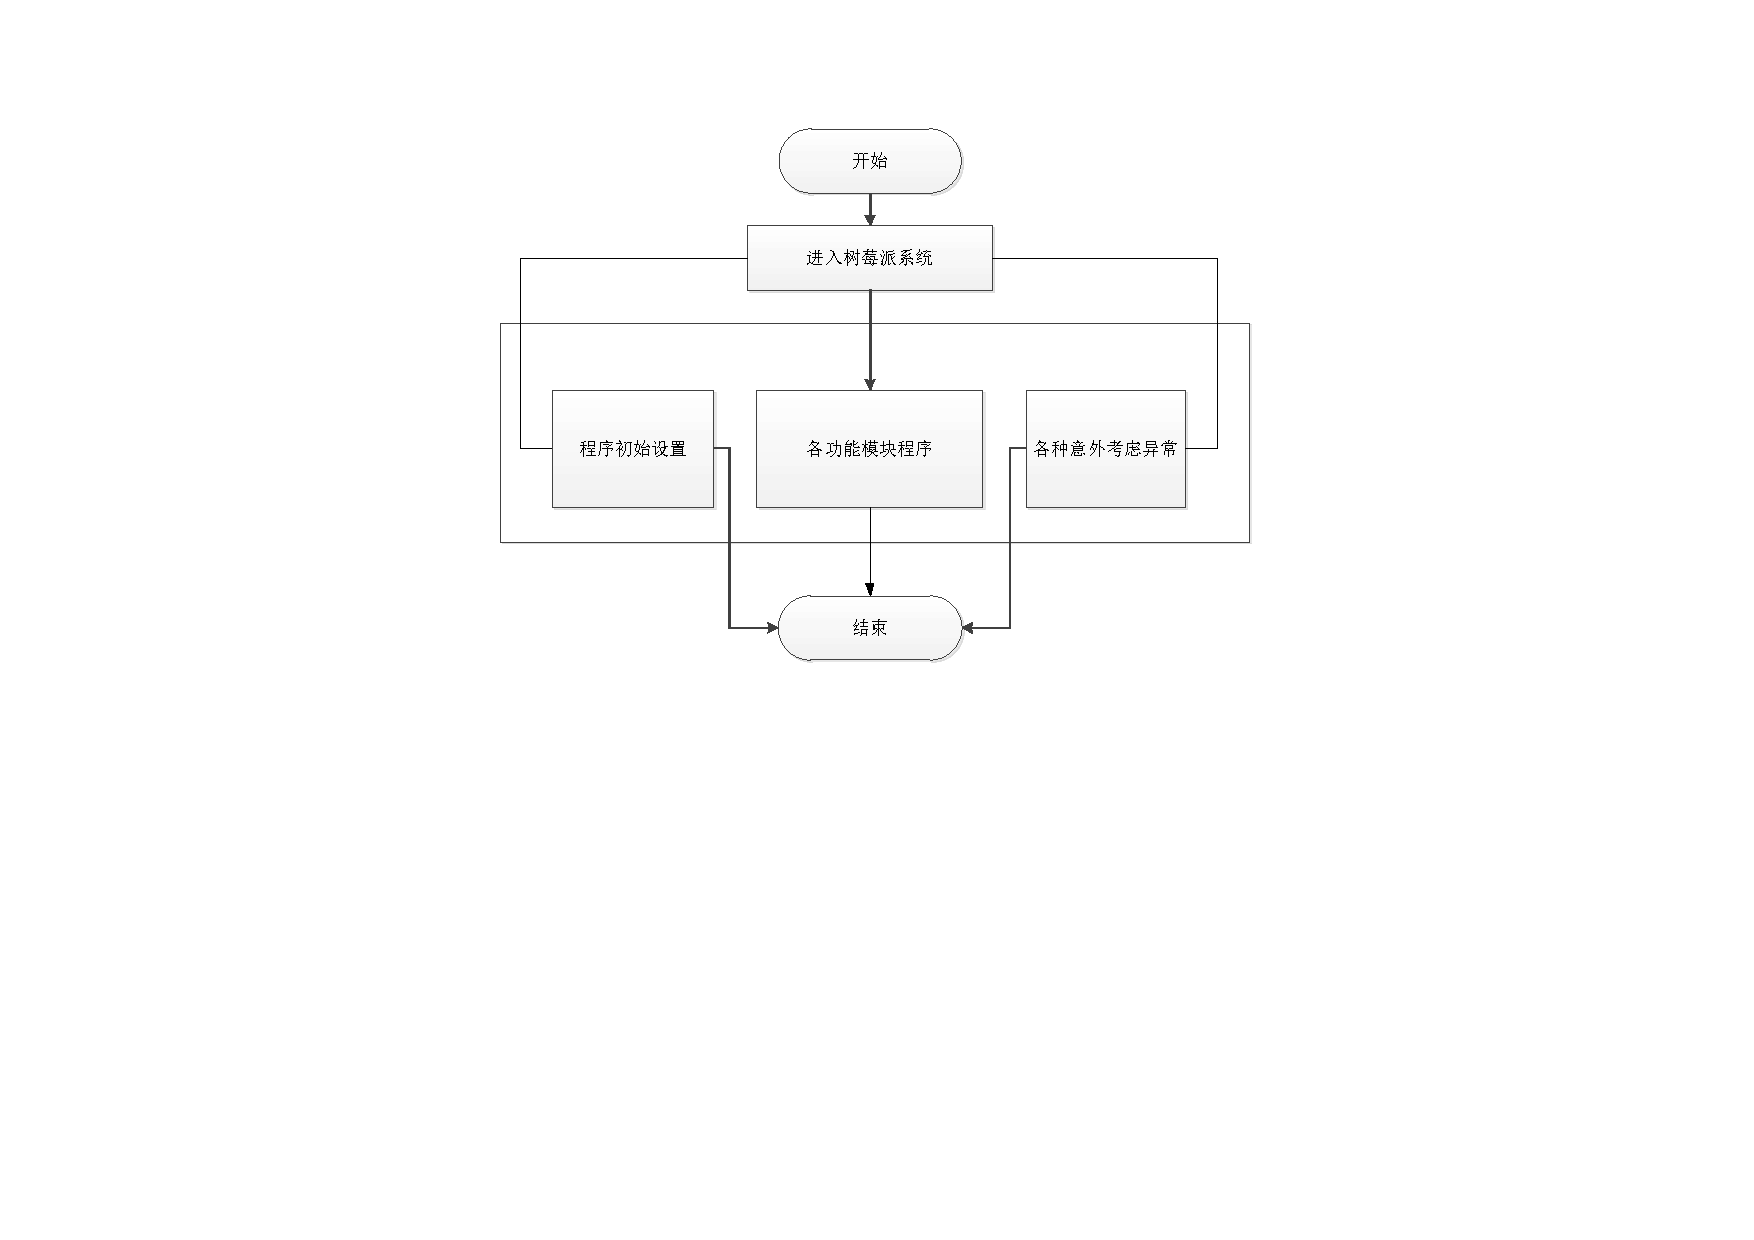
\includegraphics[width=\textwidth]{figure/software-7.pdf}
	\caption{进出库总体任务分析流程图}\label{fig:进出库总体任务分析流程图}
\end{figure}

\subsubsection{程序初始值设置(附录\ref{apdx:__init__.py}、附录\ref{apdx:config.py})}
程序首先定义了电机的管脚N1、N2、N3与N4分别为GPIO(29)、GPIO(31)、GPIO(33)和GPIO(35)。杆前红外线的避障管脚AvoidSensorfor定义为GPIO(40),杆后红外线的避障管脚AvoidSensorbac定义为GPIO(38)。程序还定义了电机四个管脚与两个红外管脚的GPIO口初始化程序。

\subsubsection{电机不同运转状态设置(附录\ref{apdx:motor.py})}
在motor.py中,定义了电机的不同运转状态程序,第一个函数SetStep()是定义电机四个管脚的输出电平,电机顺时针旋转、逆时针转动以及停止都需要调用该函数。后三个函数调用SetStep()时,SetStep()的设置得需要遵循如表4-1的步进电机驱动原理表,每次将四个GPIO端口按表4-1的步进电机驱动原理表依次设置好电平后,可以通过设置sleep()函数的时间来控制转速与方向,这样后三个函数便可以通过设置SetStep()分别实现顺时针旋转、逆时针旋转与停止。

\subsubsection{相机拍照传送(附录\ref{apdx:camera.py})}
相机拍照部分写成三个函数:capture、detect、capture\_detect。主程序里主要运行capture\_detect(),该函数里包括capture(path)与返回detect(path)。该函数运行时,调用capture(path)捕捉到照片存放到本地当前目录,文件设为image.jpg,然后返回capture(path),capture(path)将当前目录的照片发送至车牌识别云端,若从云端返回的车牌号为空,则返回0;若不为空,则返回该车牌号码。

\subsubsection{树莓派与服务器的通信(附录\ref{apdx:CarEnter.py}、附录\ref{apdx:CarOut.py})}
\begin{enumerate}
    \item 树莓派与车牌识别云端的通信:将树莓派拍下的图片作为写入字典中,然后传给传给requests.post()的参数,最后用json.loads()解码json数据;
    \item 树莓派与停车管理系统云端的通信requests.get()用于请求目标网站,类型是一个HTTPresponse类型,这里的request获取的是剩余车位的值。
\end{enumerate}

\subsubsection{车入库具体流程代码分析(附录\ref{apdx:CarEnter.py}、附录\ref{apdx:CarOut.py})}
检测车进:红外模块的避障引脚一旦出现低电平,则需要摄像头开启抓捕拍照,而且仅仅拍一张照片,将其存放到树莓派本地。紧接着照片被送往云端识别,会立即返回车的车牌号码。可能会出现未识别的情况,只要车不退回,系统会一直拍照直至能够产生车牌号码,除非用户自己离开系统放弃拍照。若产生正确的照片会被发往停车管理系统云端,返回剩余车位不为0时则杆立即抬起,车开始开进车库,第二个红外模块检测到车身时直至检测不到杆落下。

检测车出:出库程序运行时,当红外模块检测到车身时,则摄像头开启抓捕拍照。类似于车进库的操作,照片被送往云端识别,云端会返回车的号码。若是没有识别会会一直识别,若是长久不能识别,车主此时必须打电话给管理员。若是车牌识别成功,会立即发往停车管理系统云端,云端返回一个SVG字符串格式的二维码。

在本地将此格式转换为图片格式即为付款二维码。车主需要付款扫二维码并付款成功后杆才可抬起,离开的时候第二个红外模块第一次检测到车身不落杆,直到
避障管脚输出True时,杆才开始落下,此时车已经安全离开。


\subsection{车牌识别算法实现}\label{车牌识别算法实现}
\subsubsection{模型资源说明}
\begin{itemize}
	\item cascade.xml:检测模型 - 目前效果最好的cascade检测模型
	\item cascade\_lbp.xml:召回率效果较好,但其错检太多
	\item char\_chi\_sim.h5:Keras模型-可识别34类数字和大写英文字 使用14W样本训练
	\item char\_rec.h5:Keras模型-可识别34类数字和大写英文字 使用7W样本训练
	\item ocr\_plate\_all\_w\_rnn\_2.h5:基于CNN的序列模型
	\item ocr\_plate\_all\_gru.h5:基于GRU的序列模型从OCR模型修改,效果目前最好但速度较慢,需要20ms。
	\item plate\_type.h5:用于车牌颜色判断的模型
	\item model12.h5:左右边界回归模型
\end{itemize}

\subsubsection{Python依赖}
\begin{itemize}
	\item Keras (>2.0.0)
	\item Theano(>0.9) or Tensorflow(>1.1.x)
	\item Numpy (>1.10)
	\item Scipy (0.19.1)
	\item OpenCV(>3.0)
	\item Scikit-image (0.13.0)
	\item PIL
\end{itemize}

\subsubsection{参数说明}
\begin{itemize}
	\item detect\_path: 被检测图片的路径,default = None;
	\item cascade\_model\_path: 用于object detection的模型文件路径default = model/ cascade.xml;
	\item mapping\_vertical\_model\_path: 用左右边界回归模型文件路径default = model/model12.h5;
	\item ocr\_plate\_model\_path: 用于检测车牌中的文字default = model/ ocr\_plate\_all\_gru.h5;
	\item result\_save\_folder\_path: 识别结果图片存储路径folder (None表示不存储)default = None。
\end{itemize}

\subsubsection{源码解析}
\begin{enumerate}[label=\arabic*、]
	\item {\bf 入口文件 demo.py(附录\ref{apdx:demo.py})}

	      opencv2的imread函数导入图片, 返回的是Mat类型。HyperLPRLite.py中的LPR类构造函数导入model, 参数就是训练好的三个模型文件,分别是:
	      \begin{itemize}
		      \item model/cascade.xml;
		      \item model/model12.h5;
		      \item model/ocr\_plate\_all\_gru.h5
	      \end{itemize}

	\item {\bf HyperLPRLite.py(附录\ref{apdx:HyperLPRLite.py})}
	
	      参数 model\_detection 就是文件 model/cascade.xml。用到了 opencv2的CascadeClassifier()函数 cv2.CascadeClassifier(),参数输入.xml或者.yaml文件加载模型。

	\item {\bf 基于Haar特征的级联分类器用于物体检测的模型}
	
	      model.SImpleRecognizePlateByE2E()函数(附录\ref{apdx:SImpleRecognizePlateByE2E})
		  输入为一个Mat类型的图片,输出为识别的车牌字符串以及可信度confidence,该函数定义在 HyperLPRLite.py(附录\ref{apdx:HyperLPRLite.py})。其中detectPlateRough()函数(附录\ref{apdx:detectPlateRough})是返回图像中所有车牌的边框在图片中的bbox,返回值是一个表示车牌区域坐标边框的list。for循环中,对于每个识别出来的车牌用到filemappingVertical()(附录\ref{apdx:filemappingVertical})
		  
	      输入参数:
	      \begin{itemize}
		      \item image\_gray: 一个rgb图像,Mat类型;
		      \item resize\_h: 重新设定的图像大小;
		      \item top\_bottom\_padding\_rate: 表示要裁剪掉图片的上下部占比。
	      \end{itemize}

	\item {\bf detectPlateRough()函数(附录\ref{apdx:detectPlateRough})}
	
	      这个函数实现的功能如下:
	      \begin{enumerate}
		      \item resize图像大小:cv2.resize函数;
		      \item 裁剪图片:输入的top\_bottom\_padding\_rate如果是0.1,那么上面裁剪掉0.1*height,下面也裁剪掉0.1*height;
		      \item 将图像从rgb转化为灰度 cv2.cvtColor函数,cv2.COLOR\_RGB2GRAY;
		      \item 根据前面的cv2.CascadeClassifier()物体检测模型(3),输入image\_gray灰度图像,边框可识别的最小size,最大size,输出得到车牌在图像中的offset,也就是边框左上角坐标( x, y )以及边框高度( h )和宽度( w );
		      \item 对得到的车牌边框的bbox进行扩大,也就是宽度左右各扩大0.14倍,高度上下各扩大0.15倍;
		      \item 返回图片中所有识别出来的车牌边框bbox,这个list作为返回结果。
	      \end{enumerate}


	\item {\bf filemappingVertical函数(附录\ref{apdx:filemappingVertical})}
	
	      输入参数:裁剪的车牌区域图像(Mat类型),rect也是裁剪的车牌部分的图像(Mat类型)

	      实现功能:
	      \begin{enumerate}
		      \item 将原来车牌图像resize大小:66*16*3;
		      \item 将原来灰度图颜色通道[0, 255]转化为float类型[0,1];
		      \item 将输入66*16(float),输入进模型进行测试。
	      \end{enumerate}

	\item {\bf ModelFineMapping模型(附录\ref{apdx:ModelFineMapping})}
	
	      model\_finemapping()函数(附录\ref{apdx:model_finemapping})实现keras网络模型对车牌的左右边界进行回归;通过modelFineMapping.loadweights()函数加载模型文件;通过modelFineMapping.predict输出网络结果。

	      输入:16*66*3 tensor

	      输出:长度为2的tensor

	\item {\bf ocr识别(附录\ref{apdx:ocr})}
	
	      对于每个车牌区域的for循环中,经过fineMappingVertical处理后输入到recognizeOne函数(见附录\ref{apdx:recognizeOne})进行ocr识别。

	\item {\bf modelSecRec模型}
	
		  基于GRU的序列模型从OCR模型中修改的网络模型。
		  
		  model\_sec\_rec函数(附录\ref{apdx:model_sec_rec})输入model\_path为模型weights文件路径;ocr部分的网络模型(keras模型)。
		  
		  输入层:164*48*3的tensor
		  
	      输出层:长度为7 的tensor,类别有len(chars)+1种(附录\ref{apdx:chars})

\end{enumerate}


\subsection{云服务实现}
\subsubsection{微服务架构}
云端的微服务系统配置如表\ref{tab:微服务系统配置表}。它们之间的关系如图\ref{fig:微服务系统关系图}所示。各微服务之间通过Docker内部DNS互相通信,其中node、python、alipay三个微服务可以通过主机端口映射从外部网络访问;承担数据存储的mysql服务和车牌识别记录的python微服务的系统数据通过虚拟磁盘挂载存储于物理主机上,保证数据的持久性。
\begin{table}[htbp]
	\setstretch{1.5}
	\centering
	\caption{微服务系统配置表}
	\begin{tabular}{|c|c|c|c|}
		\hline
		微服务名称 & 操作系统 & 应用软件     & 功能                  \\
		\hline
		node       & alpine   & node 8.16.0  & 道闸控制微服务        \\
		\hline
		mysql      & debian   & MySQL 8.0.16 & 关系型硬盘数据库      \\
		\hline
		redis      & debian   & redis 5.0.5  & 非关系型内存数据库    \\
		\hline
		python     & debian   & python 3.7.3 & 车牌识别微服务        \\
		\hline
		alipay     & alpine   & node 8.16.0  & 付款管理微服务        \\
		\hline
		物理主机   & ubuntu   & docker       & 微服务控制台/文件系统 \\
		\hline
	\end{tabular}
	\label{tab:微服务系统配置表}
\end{table}

\begin{figure}[htbp]
	\centering
	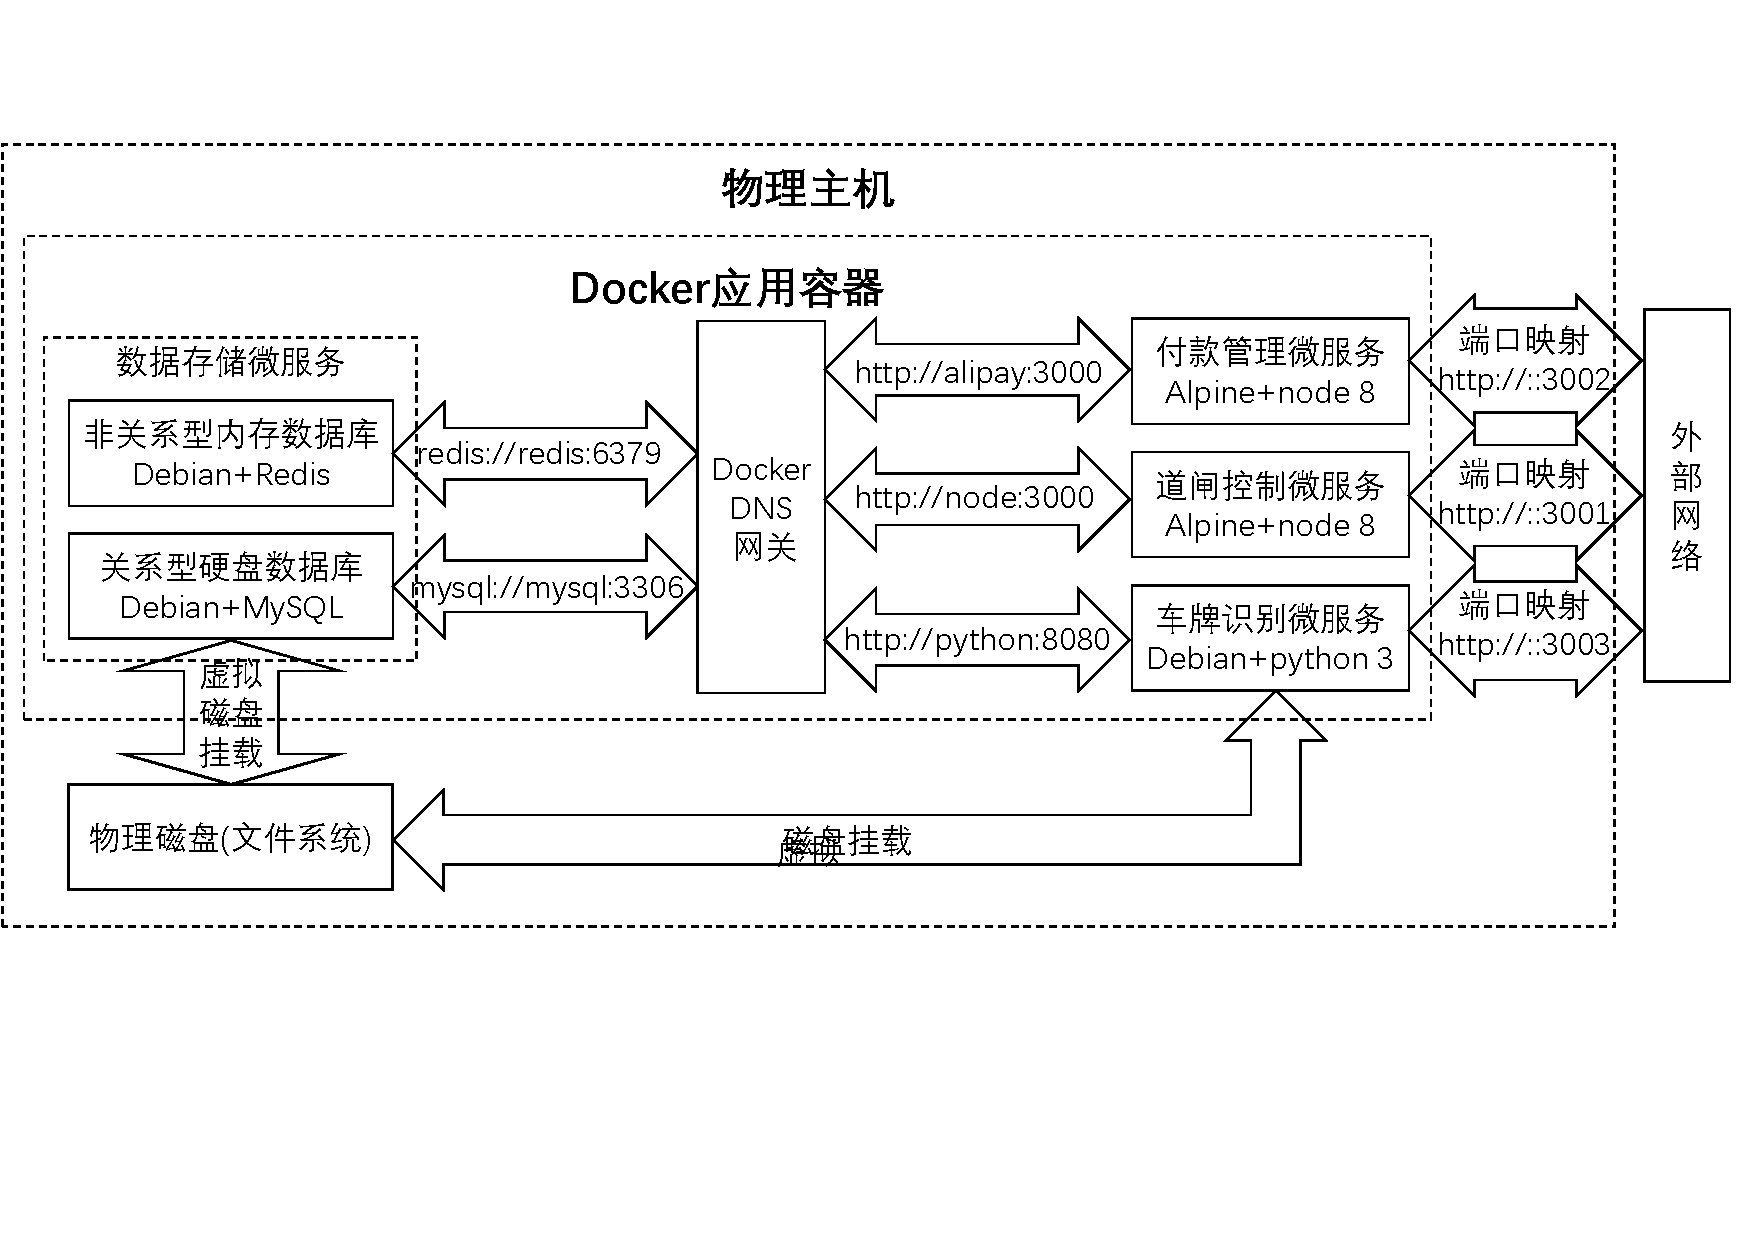
\includegraphics[width=\textwidth]{figure/docker-all.pdf}
	\caption{微服务系统关系图}\label{fig:微服务系统关系图}
\end{figure}

\subsubsection{MySQL数据库结构}
在MySQL数据库中,停车记录、付款记录和识别记录分别存储于三个数据表中:
\begin{itemize}
	\item 停车记录(表\ref{tab:停车记录表}):记录时间、车牌号和动作,其中动作包含“进入”和“离开”两种;
	      \begin{table}[htbp]
		      \setstretch{1.5}
		      \centering
		      \caption{停车记录表}
		      \begin{tabular}{|c|c|}
			      \hline
			      字段名称 & 数据类型   \\
			      \hline
			      时间     & datetime   \\
			      \hline
			      车牌号   & varchar(7) \\
			      \hline
			      动作     & boolean    \\
			      \hline
		      \end{tabular}
		      \label{tab:停车记录表}
	      \end{table}
	\item 付款记录(表\ref{tab:付款记录表}):记录时间、车牌号和付款金额;
	      \begin{table}[htbp]
		      \setstretch{1.5}
		      \centering
		      \caption{付款记录表}
		      \begin{tabular}{|c|c|}
			      \hline
			      字段名称 & 数据类型   \\
			      \hline
			      时间     & datetime   \\
			      \hline
			      车牌号   & varchar(7) \\
			      \hline
			      金额     & double     \\
			      \hline
		      \end{tabular}
		      \label{tab:付款记录表}
	      \end{table}
	\item 识别记录(表\ref{tab:识别记录表}):记录时间、图片路径和识别结果;
	      \begin{table}[htbp]
		      \setstretch{1.5}
		      \centering
		      \caption{识别记录表}
		      \begin{tabular}{|c|c|}
			      \hline
			      字段名称 & 数据类型     \\
			      \hline
			      时间     & datetime     \\
			      \hline
			      图片     & varchar(255) \\
			      \hline
			      识别结果 & json         \\
			      \hline
		      \end{tabular}
		      \label{tab:识别记录表}
	      \end{table}
\end{itemize}

\subsubsection{Redis数据库结构}\label{Redis数据库结构}
原则上说,所有需要快速即时更新的数据都要存储于Redis数据库中以保证速度。按照\ref{云服务设计}节所给出的设计方案,系统主要的实时性负担在于出口道闸处的订单状态更新和网页客户端的即时更新,因此可以将系统内付款订单的状态、车辆的状态和客户端更新标志位存入Redis数据库中。
\begin{enumerate}[label=\bf{\arabic*、}]
	\item {\bf 付款订单状态和车辆状态的存储方式}
	
	      车辆的状态可以分三种:
	      \begin{itemize}
		      \item 已停车:车牌在入口道闸成功识别但没有在出口道闸识别;
		      \item 付款中:车牌在出口道闸成功识别但没有完成付款;
		      \item 已离开:出口道闸成功识别并已完成付款。
	      \end{itemize}

	      对这三种状态的保存可以通过Redis键值对和数组两个结构实现。将车辆的进入时间与其车牌号匹配并以键值方式存入Redis数据库,将正在付款的车辆以数组方式存入一个Redis数组,车辆的三种状态就可以表示如下:
	      \begin{itemize}
		      \item 已停车:Redis键值对数据库中存有该车牌号对应的进入时间;
		      \item 付款中:Redis队列中存有该车牌号;
		      \item 已离开:Redis队列中没有该车牌号且Redis键值对数据库中也没有该车牌号对应的进入时间。
	      \end{itemize}
	      从而能同时达到存储车辆状态和订单状态的目的,并且还能为出口处的金额计算加速

	\item {\bf 客户端更新标志位的存储方式}
	
	考虑到实际应用中客户端可能被同时多次开启,因此需要为每个保持长轮询的客户端都设置一个单独的更新标志位,每个标志位都只取01二值,因此可以以Redis hash表的方式进行存储。每当有车辆状态的更新时,hash表中所有的客户端标志位都同时进行更新;而在进行长轮询时,每个客户端的请求处理程序都只查看并修改自己客户端的标志位,从而能达到多客户端同时异步更新的效果。

\end{enumerate}

\subsubsection{车牌识别微服务的实现}
车牌识别微服务实际上就是对\ref{车牌识别算法实现}中实现的车牌识别算法的封装。由于识别程序由python写就,因此选用python实现车牌识别微服务。在python中常用的服务器封装方式是http.server类,在该类中定义doPost()方法,在该方法中对图像识别请求进行处理接收,并调用\ref{车牌识别算法实现}中实现的车牌识别算法对上传的图像进行识别,即完成对车牌识别算法的封装;在每次识别完成后,都将识别图像存储与文件系统中,并在MySQL数据库识别记录表中写入图片路径和识别结果,即可完成对车牌识别情况的记录。其微服务应用核心代码如附录\ref{apdx:车牌识别微服务核心代码}所示。

\subsubsection{付款管理微服务的实现}
由\ref{云服务设计}节给出的设计方案,付款管理微服务不能与系统中的其他任何微服务有依赖关系,因此其所有的操作都必须在微服务内部进行。因此对于\ref{付款管理微服务}中给出的付款管理功能运行流程,可以使用node实现如下接口:

\begin{itemize}
	\item /create:创建支付订单、返回订单信息。当收到创建订单的请求后,使用node中的随机数生成算法生成一串随机数字(不能与系统内的其他订单重复)作为订单编号,以订单编号为键,支付信息为值存入一个全局数组中,并向请求方返回这个订单编号作为订单信息;
	\item /pay:用户支付。当用户从商家处收到订单信息(订单号)后,即向此接口传递订单信息从而发起支付请求,付款管理服务完成支付请求后将从全局数组中删除订单编号对应的订单信息;
	\item /ispay:轮询支持。轮询请求方在使用此接口查询支付情况时需带上要查询的订单编号,系统根据这个编号查询全局数组中是否还存有该订单编号,若有则说明支付未完成,反之说明支付完成,向请求方返回“支付完成”信息。
\end{itemize}

\subsubsection{道闸控制微服务的实现}
按照\ref{道闸控制微服务}节给出的设计方案,道闸控制微服务可以使用node实现如下功能:

\begin{enumerate}[label=\bf{\arabic*、}]
	\item {\bf 控制入口道闸}

	接口列表:

	\begin{itemize}
		\item /enter:接收车牌号返回“放行”(字符串"yes")或“不放行”(字符串"no")。
	\end{itemize}

	入口道闸的实现比较简单,服务端只需要在收到入口道闸终端向/enter接口发送的请求后按照剩余车位有无返回“放行”或“不放行”信息并在Redis键值数据库和MySQL停车记录表中写入车辆进入时间即可。因此可以设置一个全局变量,该变量在服务初始化时载入,初始值为停车场内车辆总数;每当有入口道闸终端的请求到达时让该变量减一、有车辆从出口道闸离开时令该变量加一,以此实现剩余车位计数和判断。

	\item {\bf 控制出口道闸}

	接口列表:

	\begin{itemize}
		\item /exit:接收车牌号返回支付订单信息;
		\item /ispay:长轮询接口,接收车牌号,查询订单支付情况。
	\end{itemize}
	
	出口道闸的运行可以分为一前一后两个请求。
	
	首先在出口道闸终端处识别车牌后,终端通过一个请求向服务器/exit接口发送车辆信息,服务器计算该车辆的应付金额后,再通过网络向付款管理微服务发起创建订单请求,将获取到订单信息返回到终端进行显示供用户支付。

	随后,出口道闸终端将向/ispay接口发起一个长轮询连接道闸控制服务,道闸控制服务在后台对订单支付状态进行短轮询,直到付款管理微服务返回了“支付完成”信息,按照支付消息经由长轮询连接向道闸终端发送“放行”或“不放行”(字符串"ok")或“支付取消”(字符串"no")指令。

	由以上两个请求即可实现完整的出口道闸控制功能。此外,在/exit请求中创建订单完成后将车辆信息放入Redis队列,即可将车辆状态从“已停车”改变为“付款中”;在/ispay请求的“支付完成”信息到达时车辆信息从Redis队列和键值数据库中删除,即可将车辆状态从“付款中”改变为“已离开”;且每当车辆状态从“付款中”改变为“已离开”后,将付款车牌号、时间以及金额和“离开”动作分别写入MySQL付款记录表和停车记录表中,即可实现停车历史和付款历史的记录。

	\item {\bf 支持客户端网页上停车情况的即时更新}
	
	接口列表:
	\begin{itemize}
		\item /updated:长轮询接口,接收客户端的连接请求,返回更新数据指令;
		\item /getCurrentCars:获取当前车辆信息。
	\end{itemize}

	由\ref{道闸控制微服务}节给出的网页停车情况的即时更新需求以及\ref{Redis数据库结构}中给出的标志位处理方式,可以得到客户端网页的即时更新以及服务器支持的实现方式:

	\begin{itemize}
		\item 客户端:使用jQuery的Ajax方法从服务器端获取数据,使用渐进式框架Vue.js将数据与页面元素绑定。不断向服务端/updated接口发起Ajax长轮询请求,当收到更新指令后向/getCurrentCars请求当前车辆信息并完成页面显示的刷新;
		\item 服务端:每当一个新的客户端的客户端发起了连接请求(任意连接请求)时,为这个客户端分配一个唯一的编号写入cookie中,同时还将这个编号写入Redis客户端更新标志位hash表。当客户端向/updated接口发起长轮询时,服务端不断短轮询Redis客户端更新标志位hash表中长轮询客户端cookie值对应的hash存储值,直到该值置1,则向客户端发送更新指令,并将该位置0。按照\ref{Redis数据库结构}中给出的Redis客户端更新标志位hash表更新方式进行标志位更新,即可实现客户端网页上停车情况的即时更新支持。
	\end{itemize}

	\item {\bf 获取道闸放行历史记录}
	
	相关接口:
	\begin{itemize}
		\item /index/getHistoryCars:获取系统中的所有车牌号,返回值为一记录车牌号的JSON数组;
		\item /index/getCarHistorys:输入值为车牌号,获取该车牌号在停车记录表中的所有记录,返回值为时间和停车记录组成的二维JSON数组;
		\item /index/getCarPayments:输入值为车牌号,获取该车牌号在付款记录表中的所有记录,返回值为时间和付款金额组成的二维JSON数组;
		\item /index/getDetects:获取所有的识别记录,返回值为时间、图片url和识别结果组成的二维JSON数组。
	\end{itemize}
	
\end{enumerate}

\section{总结}
\subsection{设计结果}
整个系统能稳定运行且完全符合设计要求。

\subsection{遇到的问题}
\begin{enumerate}
	\item 刚开始在设计过程中,自己对于电机的设计存在疏漏之处,旋转时不是在0至90度之间转动,而是只要红外避障管脚输入合适,电机会转任意角度,这显然不符合实际;
	
	改进:设置角度标志位,只要起杆过一次,它也就不会再起杆了,除非杆已经落下。

	\item 杆前红外线检测到车进入时比较容易控制起杆,因为是车头先碰到,是符合常理的。但是离开时需要车尾完全离开时才行,而程序也是车头先碰到再落杆;
	
	改进:需要在落杆程序那里设置死循环,杆后红外第一次检测到不落杆,直至检测不到再落杆。

	\item 过程中发现树莓派的拍照功能不是很好,传送给云端的照片有很多无法识别,但是程序没有这种应对措施;
	
	改进:添加标志位可以解决问题,若发现系统无法识别的情况,应该一直识别直到识别出车牌为止,若车主不想等可以离开,系统则等待下一辆车的进库。
\end{enumerate}

\subsection{心得体会}
\begin{enumerate}
	\item 以团队的形式进行的综合课程设计极大地提高了班级凝聚力;
	\item 在互相协作中掌握了大型项目的规划和协调能力;
	\item 精进了大家的代码水平;
	\item 对物联网的理解更进一步。
\end{enumerate}

\newpage
\section*{附录}\addcontentsline{toc}{section}{附录}\appendix
\section{demo.py(部分)}\label{apdx:demo.py}
\begin{lstlisting}[language=python]
import HyperLPRLite as pr
import cv2
import numpy as np

grr = cv2.imread("images_rec/2_.jpg")
model = pr.LPR("model/cascade.xml", "model/model12.h5", "model/ocr_plate_all_gru.h5")
for pstr, confidence, rect in model.SimpleRecognizePlateByE2E(grr):
	if confidence > 0.7:
		image = drawRectBox(grr, rect, pstr + " " + str(round(confidence, 3)))
		print "plate_str:"
		print pstr
		print "plate_confidence"
		print confidence
cv2.imshow("image", image)
cv2.waitKey(0)
\end{lstlisting}

\section{HyperLPRLite.py(部分)}\label{apdx:HyperLPRLite.py}
\begin{lstlisting}[language=python]
class LPR():
def __init__(self,model_detection,model_finemapping,model_seq_rec):
	self.watch_cascade = cv2.CascadeClassifier(model_detection)
	self.modelFineMapping = self.model_finemapping()
	self.modelFineMapping.load_weights(model_finemapping)
	self.modelSeqRec = self.model_seq_rec(model_seq_rec)
\end{lstlisting}

\section{model.SImpleRecognizePlateByE2E()}\label{apdx:model.SImpleRecognizePlateByE2E}
\begin{lstlisting}[language=python]
for pstr,confidence,rect in model.SimpleRecognizePlateByE2E(grr):
	if confidence>0.7:
		image = drawRectBox(grr, rect, pstr+" "+str(round(confidence,3)))
		print "plate_str:"
		print pstr
		print "plate_confidence"
		print confidence
\end{lstlisting}

\section{SImpleRecognizePlateByE2E()}\label{apdx:SImpleRecognizePlateByE2E}
\begin{lstlisting}[language=python]
def SimpleRecognizePlateByE2E(self, image):
images = self.detectPlateRough(image, image.shape[0], top_bottom_padding_rate=0.1)
res_set = []
for j, plate in enumerate(images):
	plate, rect = plate
	image_rgb, rect_refine = self.finemappingVertical(plate, rect)
	res, confidence = self.recognizeOne(image_rgb)
	res_set.append([res, confidence, rect_refine])
return res_set
\end{lstlisting}

\section{detectPlateRough()}\label{apdx:detectPlateRough}
\begin{lstlisting}[language=python]
def detectPlateRough(self, image_gray, resize_h=720, en_scale=1.08, top_bottom_padding_rate=0.05):
if top_bottom_padding_rate > 0.2:
	print("error:top_bottom_padding_rate > 0.2:", top_bottom_padding_rate)
	exit(1)
height = image_gray.shape[0]
padding = int(height * top_bottom_padding_rate)
scale = image_gray.shape[1] / float(image_gray.shape[0])
image = cv2.resize(image_gray, (int(scale * resize_h), resize_h))
image_color_cropped = image[padding:resize_h - padding, 0:image_gray.shape[1]]
image_gray = cv2.cvtColor(image_color_cropped, cv2.COLOR_RGB2GRAY)
watches = self.watch_cascade.detectMultiScale(image_gray, en_scale, 2, minSize=(36, 9), maxSize=(36 * 40, 9 * 40))
cropped_images = []
for (x, y, w, h) in watches:
	x -= w * 0.14
	w += w * 0.28
	y -= h * 0.15
	h += h * 0.3
	cropped = self.cropImage(image_color_cropped, (int(x), int(y), int(w), int(h)))
	cropped_images.append([cropped, [x, y + padding, w, h]])
return cropped_images
\end{lstlisting}

\section{filemappingVertical()}\label{apdx:filemappingVertical}
\begin{lstlisting}[language=python]
def finemappingVertical(self, image, rect):
resized = cv2.resize(image, (66, 16))
resized = resized.astype(np.float) / 255
res_raw = (np.array([resized]))[0]
res = res_raw * image.shape[1]
res = res.astype(np.int)
H, T = res
H -= 3
if H < 0:
	H = 0
T += 2;
if T >= image.shape[1] - 1:
	T = image.shape[1] - 1
rect[2] -= rect[2] * (1 - res_raw[1] + res_raw[0])
rect[0] += res[0]
image = image[:, H:T + 2]
image = cv2.resize(image, (int(136), int(36)))
return image, rect
\end{lstlisting}

\section{ModelFineMapping模型}\label{apdx:ModelFineMapping}
\begin{lstlisting}[language=python]
class LPR():
    def __init__(self,model_detection,model_finemapping,model_seq_rec):
        self.watch_cascade = cv2.CascadeClassifier(model_detection)
        self.modelFineMapping = self.model_finemapping()
        self.modelFineMapping.load_weights(model_finemapping)
        self.modelSeqRec = self.model_seq_rec(model_seq_rec)
\end{lstlisting}

\section{model\_finemapping()}\label{apdx:model_finemapping}
\begin{lstlisting}[language=python]
def model_finemapping(self):
input = Input(shape=[16, 66, 3])
x = Conv2D(10, (3, 3), strides=1, padding='valid', name='conv1')(input)
x = Activation("relu", name='relu1')(x)
x = MaxPool2D(pool_size=2)(x)
x = Conv2D(16, (3, 3), strides=1, padding='valid', name='conv2')(x)
x = Activation("relu", name='relu2')(x)
x = Conv2D(32, (3, 3), strides=1, padding='valid', name='conv3')(x)
x = Activation("relu", name='relu3')(x)
x = Flatten()(x)
output = Dense(2, name="dense")(x)
output = Activation("relu", name='relu4')(output)
model = Model([input], [output])
return model
\end{lstlisting}

\section{ocr识别}\label{apdx:ocr}
\begin{lstlisting}[language=python]
for j, plate in enumerate(images):
plate, rect = plate
image_rgb, rect_refine = self.finemappingVertical(plate, rect)
res, confidence = self.recognizeOne(image_rgb)
res_set.append([res, confidence, rect_refine])
\end{lstlisting}

\section{recognizeOne()}\label{apdx:recognizeOne}
\begin{lstlisting}[language=python]
def recognizeOne(self, src):
x_tempx = src
x_temp = cv2.resize(x_tempx, (164, 48))
x_temp = x_temp.transpose(1, 0, 2)
y_pred = self.modelSeqRec.predict(np.array([x_temp]))
y_pred = y_pred[:, 2:, :]
return self.fastdecode(y_pred)
\end{lstlisting}

\section{model\_sec\_rec()}\label{apdx:model_sec_rec}
\begin{lstlisting}[language=python]
def model_seq_rec(self, model_path):
width, height, n_len, n_class = 164, 48, 7, len(chars) + 1
rnn_size = 256
input_tensor = Input((164, 48, 3))
x = input_tensor
base_conv = 32
for i in range(3):
	x = Conv2D(base_conv * (2 ** (i)), (3, 3))(x)
	x = BatchNormalization()(x)
	x = Activation('relu')(x)
	x = MaxPooling2D(pool_size=(2, 2))(x)
conv_shape = x.get_shape()
x = Reshape(target_shape=(int(conv_shape[1]), int(conv_shape[2] * conv_shape[3])))(x)
x = Dense(32)(x)
x = BatchNormalization()(x)
x = Activation('relu')(x)
gru_1 = GRU(rnn_size, return_sequences=True, kernel_initializer='he_normal', name='gru1')(x)
gru_1b = GRU(rnn_size, return_sequences=True, go_backwards=True, kernel_initializer='he_normal', name='gru1_b')(x)
gru1_merged = add([gru_1, gru_1b])
gru_2 = GRU(rnn_size, return_sequences=True, kernel_initializer='he_normal', name='gru2')(gru1_merged)
gru_2b = GRU(rnn_size, return_sequences=True, go_backwards=True, kernel_initializer='he_normal', name='gru2_b')(
	gru1_merged)
x = concatenate([gru_2, gru_2b])
x = Dropout(0.25)(x)
x = Dense(n_class, kernel_initializer='he_normal', activation='softmax')(x)
base_model = Model(inputs=input_tensor, outputs=x)
base_model.load_weights(model_path)
return base_model
\end{lstlisting}

\section{chars}\label{apdx:chars}
\begin{lstlisting}[language=python]
chars = [
    u"京", u"沪", u"津", u"渝", u"冀", u"晋", u"蒙", u"辽", u"吉", u"黑",
    u"苏", u"浙", u"皖", u"闽", u"赣", u"鲁", u"豫", u"鄂", u"湘", u"粤",
    u"桂", u"琼", u"川", u"贵", u"云", u"藏", u"陕", u"甘", u"青", u"宁",
    u"新", u"0", u"1", u"2", u"3", u"4", u"5", u"6", u"7", u"8", u"9", u"A",
    u"B", u"C", u"D", u"E", u"F", u"G", u"H", u"J", u"K", u"L",u"M",u"N",
    u"P", u"Q", u"R", u"S", u"T", u"U", u"V", u"W", u"X", u"Y", u"Z",u"港",
    u"学", u"使",u"警",u"澳",u"挂",u"军",u"北",u"南",u"广",u"沈",u"兰",u"成", 
    u"济",u"海",u"民",u"航",u"空"]
\end{lstlisting}

\section{config.py}\label{apdx:config.py}
\begin{lstlisting}[language=python]
IN1 = 29
IN2 = 31
IN3 = 33
IN4 = 35
AvoidSensorfor = 40
AvoidSensorbac = 38
\end{lstlisting}

\section{\_\_init\_\_.py}\label{apdx:__init__.py}
\begin{lstlisting}[language=python]
import RPi.GPIO as GPIO
from .config import IN1,IN2,IN3,IN4,AvoidSensorfor,AvoidSensorbac

def setup():
    GPIO.setwarnings(False)
    GPIO.setmode(GPIO.BOARD)
    GPIO.setup(IN1, GPIO.OUT)
    GPIO.setup(IN2, GPIO.OUT)
    GPIO.setup(IN3, GPIO.OUT)
    GPIO.setup(IN4, GPIO.OUT)
    GPIO.setup(AvoidSensorfor, GPIO.IN)
    GPIO.setup(AvoidSensorbac, GPIO.IN)
    print('GPIO初始化完成')


def destroy():
    GPIO.cleanup()  # Release resource


setup()
\end{lstlisting}

\section{motor.py}\label{apdx:motor.py}
\begin{lstlisting}[language=python]
import time
import RPi.GPIO as GPIO


def setStep(w1, w2, w3, w4):
    from .config import IN1, IN2, IN3, IN4
    GPIO.output(IN1, w1)
    GPIO.output(IN2, w2)
    GPIO.output(IN3, w3)
    GPIO.output(IN4, w4)


def stop():
    print('电机stop')
    setStep(0, 0, 0, 0)


def forward(delay, steps):
    print('电机forward')
    for i in range(0, steps):
        setStep(1, 0, 0, 0)
        time.sleep(delay)
        setStep(0, 1, 0, 0)
        time.sleep(delay)
        setStep(0, 0, 1, 0)
        time.sleep(delay)
        setStep(0, 0, 0, 1)
        time.sleep(delay)


def backward(delay, steps):
    print('电机backward')
    for i in range(0, steps):
        setStep(0, 0, 0, 1)
        time.sleep(delay)
        setStep(0, 0, 1, 0)
        time.sleep(delay)
        setStep(0, 1, 0, 0)
        time.sleep(delay)
        setStep(1, 0, 0, 0)
		time.sleep(delay)
\end{lstlisting}

\section{camera.py}\label{apdx:camera.py}
\begin{lstlisting}[language=python]
import picamera
import requests
import json
camera = picamera.PiCamera()
#from hyperlpr import HyperLPR_PlateRecogntion
#import cv2


def capture(path):
    camera.capture(path)
    print('摄像头捕获图像'+path)


def detect(path):
    print('开始识别图像'+path)
    #image = cv2.imread(path)
    #id = '123456'
    #id = HyperLPR_PlateRecogntion(image)
    url1 = "http://yindaheng98.top:3003"  # 车牌识别接口地址
    files = {'file': open(path, 'rb')}
    r = requests.post(url1, {'arg': 1}, files=files)
    id = json.loads(r.text)
    print(id)  # 返回值即为识别结果
    if id == [[]]:
        return 0
    id = id[0][0][0]
    return id


def capture_detect():
    path = "image.jpg"
    capture(path)
    return detect(path)
\end{lstlisting}

\section{CarEnter.py}\label{apdx:CarEnter.py}
\begin{lstlisting}[language=python]
import RPi.GPIO as GPIO
import requests

from ParkingMoney import AvoidSensorfor, AvoidSensorbac, destroy
from ParkingMoney.motor import forward, backward, stop
from ParkingMoney.camera import capture_detect

AvoidValuefor = False
AvoidValuebac = False
LimitAngleFlag = 0


url = 'http://yindaheng98.top:3001/enter/'


def loopUp():
    global LimitAngleFlag
    AvoidValuefor = GPIO.input(AvoidSensorfor)
    if AvoidValuefor == False:
        id = capture_detect()
        if id==0:
            return
        print("入口处传数据"+url+id)
        response = requests.get(url+id)
        print("服务器返回"+response.text)
        if response.text[0:2] == 'ok':
            print("开始抬杆")
            if LimitAngleFlag == 0:
                backward(0.003, 128)  # 512 steps --- 360 angle
                LimitAngleFlag = 1
        else:
            print("出错")


def loopDown():
    global LimitAngleFlag
    print("开始落杆")
    if LimitAngleFlag == 1:
        forward(0.003, 128)  # 512 steps --- 360 angle
        LimitAngleFlag = 0


if __name__ == '__main__':
    try:
        while True:
            loopUp()
            AvoidValuebac = GPIO.input(AvoidSensorbac)
            if AvoidValuebac == False:
                print("抬杆完成")
                while True:
                    AvoidValuebac = GPIO.input(AvoidSensorbac)
                    if AvoidValuebac == True:
                        print("车已开走")
                        loopDown()
                        break

    # When 'Ctrl+C' is pressed, the child function destroy() will be  executed.
    except KeyboardInterrupt:
        destroy()
\end{lstlisting}


\section{CarOut.py}\label{apdx:CarOut.py}
\begin{lstlisting}[language=python]
import RPi.GPIO as GPIO
import requests
from cairosvg import svg2png
#import cv2


from ParkingMoney import AvoidSensorfor, AvoidSensorbac, destroy
from ParkingMoney.motor import forward, backward, stop
from ParkingMoney.camera import capture_detect

AvoidValuefor = False
AvoidValuebac = False
LimitAngleFlag = 0


url_exit = 'http://yindaheng98.top:3001/exit/'

url_ispay = 'http://yindaheng98.top:3001/ispay/'


def loopUp():
    global LimitAngleFlag
    AvoidValuefor = GPIO.input(AvoidSensorfor)
    if AvoidValuefor == False:
        id = capture_detect()
        print("出口处传数据"+url_exit+id)
        response = requests.get(url_exit+id)
        if response.text=='error':
            print('出错')
            return
        svg2png(bytestring=response.text, write_to='output.png')
        #cv2.imshow('二维码', cv2.imread('output.png'))
        print("出口处查询付款情况"+url_ispay+id)
        response = requests.get(url_ispay+id)
        print('result:'+response.text)
        if response.text == 'yes':
            print("开始抬杆")
            if LimitAngleFlag == 0:
                backward(0.003, 128)  # 512 steps --- 360 angle
                LimitAngleFlag = 1


def loopDown():
    global LimitAngleFlag
    print("开始落杆")
    if LimitAngleFlag == 1:
        forward(0.003, 128)  # 512 steps --- 360 angle
        LimitAngleFlag = 0


if __name__ == '__main__':  # Program start from here
    try:
        while True:
            loopUp()
            AvoidValuebac=GPIO.input(AvoidSensorbac)
            if AvoidValuebac==False:
                print ("111111111111!")
                while True:
                    print ("222222222!")
                    AvoidValuebac=GPIO.input(AvoidSensorbac)
                    if AvoidValuebac==True:
                        print ("3333333333!")
                        loopDown()
                        break
                       
    except KeyboardInterrupt:  # When 'Ctrl+C' is pressed, the child function destroy() will be  executed.
        destroy()
	\end{lstlisting}
\section{车牌识别微服务核心代码}\label{apdx:车牌识别微服务核心代码}
\begin{lstlisting}[language=python]
# coding=utf-8
import logging
from database import connect, rand_filename, add
import json
from hyperlpr import HyperLPR_PlateRecogntion
import cv2
import cgi
from http.server import BaseHTTPRequestHandler
import numpy as np

def rotate(n, img):
	for i in range(0, n):
		img = np.flip(np.transpose(img, axes=(1, 0, 2)), 1)
	return img

conn = None
logging.basicConfig(level=logging.DEBUG)

class PostHandler(BaseHTTPRequestHandler):
	def log_message(self, *args, **kwargs):
		fmt = 'PostHandler.log_message(%s,%s)'
		logging.debug(fmt % (str(args), str(kwargs)))

	def do_POST(self):
		global conn
		if(conn == None):
			conn = connect()
		try:
			conn.cursor()
		except:
			conn=connect()
		form = cgi.FieldStorage(
			fp=self.rfile,
			headers=self.headers,
			environ={
				'REQUEST_METHOD': 'POST',
				'CONTENT_TYPE': self.headers['Content-Type']
			}
		)
		arg = int(form['arg'].value) if 'arg' in list(form.keys()) else 0
		self.send_response(200)
		self.end_headers()

		results = []
		for field in form.keys():
			if field == 'arg':
				continue
			field_item = form[field]
			filename = rand_filename(
				conn, 32, '%s.'+form[field].filename.split('.')[-1])
			path = 'images/'+filename
			with open(path, 'wb') as f:
				f.write(form[field].value)
			img = rotate(arg, cv2.imread(path))
			print(img.shape)
			cv2.imwrite(path, img)
			print(path)
			result = HyperLPR_PlateRecogntion(img)
			results.append(result)
			add(conn, filename, json.dumps(result))
		self.wfile.write(json.dumps(results).encode('utf-8'))
		return

def StartServer():
	from http.server import HTTPServer
	sever = HTTPServer(("", 8080), PostHandler)
	sever.serve_forever()

if __name__ == '__main__':
	logging.debug('车牌识别服务启动!')
	StartServer()
	conn.close()
\end{lstlisting}

\end{document}